\documentclass[12pt,a4paper,norsk]{uiothesis}
\usepackage[norsk]{babel}
\usepackage[section]{placeins}
\usepackage{pgfplots}
%\pgfplotsset{width=7cm,compat=1.8}
\usepackage{pgfplotstable}
\usepackage{pifont}

% Norwegian parskip
\setlength{\parindent}{0pt}
\nonzeroparskip


\usepackage{tabto}
\newenvironment{tabbedenum}[1]
 {\NumTabs{#1}\inparaenum\let\latexitem\item
  \def\item{\def\item{\tab\latexitem}\latexitem}}
 {\endinparaenum}

\usepackage{minted}
\renewcommand\listingscaption{Kodesnutt}
\renewcommand\listoflistingscaption{Kodesnutter}

\author{Eivind Mikael Lindbråten}
\title{Test}

\begin{document} 
	
	\chapterstyle{uio} \pagestyle{uio} \maxsecnumdepth{subsection}

	\maketitle
	\frontmatter 
	\pagenumbering{alph} \pagenumbering{roman} \clearpage 
	
	\nocite{bringhurst1999elements} % Stilsett er basert på denne
	\chapter{Sammendrag}

Automatisk orddeling er en viktig del av dagens systemer for tekstsetting.  Dessverre skjer ikke dette uten feil. Systemene tilbyr heller ingen kontroll over hvilke typer regler som skal benyttes ved orddeling. I det norske språk har vi flere regler som kan gi opphav til delepunkt i et ord. Det kan argumenteres for at disse delepunktene er av forskjellig kvalitet, og det er derfor ønskelig å kunne ha en større kontroll over dette når en skal sette en tekst. I denne oppgaven ser vi på muligheten for implementasjon av en regelbasert tilnærming til orddelingsproblemet, som skal gi økt presisjon og økt kontroll over orddelingen. \cleardoublepage
	
	\tableofcontents \clearpage 
	\listoffigures \clearpage 
	\listoftables \clearpage
	\listoflistings
	

	\chapter*{Forord}

Automatisk orddeling er en viktig del av dagens systemer for tekstsetting. Dessverre skjer det ikke uten feil. Nærmest daglig kan vi i aviser og nettpublikasjoner se eksempler på uheldig orddeling, som fører til misvisende eller komiske ordbilder -- eksempelvis som i figur~\ref{fig:forord-doplager}. Dette vil være et økende problem i den hektiske mediehverdagen, hvor nyheter må publiseres raskt og korrekturarbeid nedprioriteres. \TeX{}\sidenote[-5]{\TeX{}, utviklet av Donald Knuth, er et program for spesifisering av layout og typografisk tekstsetting.}, og er et av de fremste, fritt tilgjengelige systemene for tekstsetting. Programmet finner omtrent 90~\% av alle lovlige delepunkter, med rundt én prosent gale delinger \cite{thoresen1993virtuelle}. I majoriteten av tilfellene trengs det kun ett delepunkt når et ord må deles ved linjeslutt. Det er derfor viktigst at antall gale delinger reduseres fremfor å finne flest mulige av de lovlige delepunktene i et ord. Sett i lys av dette fungerer \TeX{}-algoritmen godt. Et større problem er at orddelingsalgoritmen i \TeX{} først og fremst er utviklet med tanke på amerikansk-engelsk orddeling, som er basert på uttale. Systemet har ingen støtte for \term{ikke-standard orddeling}\sidenote[-11]{Ikke-standard orddeling betegner orddelingsregler som avviker fra den typiske orddelingen hvor en bindestrek skytes inn mellom to bokstaver i ordet. Et eksempel er ord som endrer stavelse ved orddeling. I tysk finnes «backen» som skal deles som «bak-ken», eller i norsk hvor «soppose» blir til «sopp-pose».}. Dette er et problem som gjelder de fleste, også kommersielle, systemer for tekstsetting. Et tredje problem er den manglende kontrollen over orddeling som tilbys i alle dagens systemer. For norsk skriftspråk har vi flere regler som kan gi opphav til delepunkter i et ord. Disse kan argumenteres for å være av varierende kvalitet. Det vil derfor være ønskelig å kunne skille mellom typer av orddelingsregler som skal benyttes ved orddeling. Vi har i hovedsak to regler for orddeling: \term{ordleddsregelen} og \term{enkonsonantregelen}. Ordleddsregelen sier at vi skal dele ord «mellom betydningsbærendebærende og/eller lett gjenkjennelige orddeler», og benyttes i hovedsak ved sammensatte ord, avledninger og bøyningsendelser. Enkonsonantregelen forteller: «uavhengig av ordets betydning, la én konsonant følge med til neste linje». \cite{vinje} Ut fra dette ser vi at orddelingen i figur~\ref{fig:forord-freskukens} er lovlig, men også uheldig. Ved å benytte ordleddsregelen ville dette vært unngått. For sammensatte ord vil ordleddsreglen, fremfor enkonsonantregelen, typisk føre til færre misvisende delinger. Men dessverre tilbyr ingen av dagens metoder for automatisk orddeling en slik grad av kontroll. I denne oppgaven ser vi nærmere på disse problemene og muligheten for å utvikle en løsning.

\marginelement[-21]{

\includegraphics[width=\marginparwidth]{content/figures/forord-doplager.jpg}
\captionof{figure}[Uheldig orddeling]{Eksempel på uheldig orddeling som fører til et komisk ordbilde. 
Faksimile, Dagbladet nett 25. september 2013.  \url{http://www.dagbladet.no/2013/09/25/nyheter/utdanning/narkotika/innenriks/29445603/}}
\label{fig:forord-doplager}
}


\marginelement[-5]{
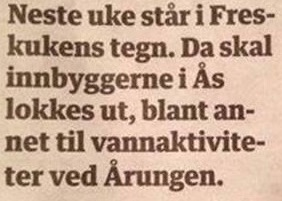
\includegraphics[width=\marginparwidth]{content/figures/forord-freskukens.jpg}
\captionof{figure}[Uheldig bruk av enkonsonantregelen]{Eksempel på uheldig bruk av enkonsonantregelen, som ga opphav til et komisk ordbilde.
Faksimile, Østlandet Blad.}
\label{fig:forord-freskukens}
}

\clearpage

Målet for oppgaven er å skissere og implementere et analytisk system, som kan dele ord etter de gjeldene reglene for orddeling, samtidig gi kontroll over reglene som skal benyttes. For å få til dette er det flere individuelle oppgaver som må løses, og systemet vil få en modulbasert arkitektur. I forbindelse med dette har jeg spesielt to spørsmål jeg ønsker svar på, og har formulert følgende problemstillinger (PS):

\begin{quote}
PS1: Hvor godt utfører modulene oppgavene sine hver for seg?
\end{quote}

Det vil være interessant å se nærmere på modulene i isolasjon med egne testkriterier og tester. Med dette vil det være mulig å identifisere svakheter i enkeltmoduler i programflyten, og kan fungere som en pekepinn på mulig videre arbeid for å forbedre programmet.

\begin{quote}
PS2: Hvor god kvalitet og kontroll får vi på orddelingen?
\end{quote}

Her ønsker vi å få svar på hvor vellykket løsningen er for å dele ord, samt hvilken eventuell økt kontroll vi kan få over orddelingsvalgene.

\section*{Takksigelser}

Først og fremst vil jeg gjerne takke min veileder Dag Langmyhr for å ha gitt så mye av sin tid og for spennende samtaler, rundt det som for mange er et smalt tema. Jeg vil også takke kjæresten min for korrekturlesning og støtte under en intens innspurt. Til sist -- takk til familie og venner for inspirasjon og gledelige stunder!

	\mainmatter 
	
	\chapter{Introduksjon}

Utviklingen av skriftspråket har vært et stort bidrag til fremgangen i vårt samfunn. Det er lett å se den enorme innvirkingen dette har hatt. Vi har gått fra å kun kunne dele idéer og tanker muntlig, eller gjennom enkle billedlige fremstillinger, til å metodisk og strukturert kunne skrive det ned og effektivt og presist kunne spre budskapet videre uten forringelse. Våre idéer vil også kunne nå mange flere mottakere samtidig og mottakere som befinner seg mer geografisk spredt. Det vi skriver ned vil også kunne bli lagret over mye lengere tidsperioder til ettertiden uten å miste detaljer i overleveringen slik som kan skje med muntlige overleveringer. Vi bygger opp et kollektivt bibliotek av idéer som vil øke vår kollektive kunnskap og som muliggjør kunnskap som bygger på annen kunnskap i større grad.

\section{Typografi, Gutenberg og orddeling}

Typografien beskjeftiger seg med utformingen og behandlingen av tekst, hvor hovedoppgavene er leselighet og tilpassning av form til innhold. En tekst ønsker å kommunisere et sett med idéer til leseren, hvor typografiens oppgave er å styrke disse idéene i teksten gjennom den visuelle utformingen. Hvis man ikke tar seg bryet med god typografi vil leseren i større grad bli distrahert og leseren vil ledes vekk fra idéene som teksten ønsker å kommunisere. Som det ofte blir sagt; «God typografi er usynlig, dårlig typografi er over alt».

Gjennom hans arbeid med 42-linjersbibelen og samtidig utviklingen av boktrykkerkunsten, fikk Johan Gutenberg (ca. 1400–1468) perfeksjonert mye av det arbeidet som inngår i typografien. Han ønsket å utvikle hurtigere teknikker for produskjon av bøker, hvor resultatet hadde minst like høy kvalitet og visuell skjønnhet som de beste håndproduserte bøkene i hans samtid. 

For at en tekst skal oppfattes som visuelt vakker og ha høy leselighet er spesielt to mål viktig å oppnå: 

Det er spesielt to mål som er viktig å strebe etter, for at en tekst skal oppfattes som estetisk og ha en høy leselighet:

\begin{items}
\item at helheten i teksten har en uniform \textit{farge}\sidenote[-2]{Farge et uttrykk som brukes til å beskrive den helhetlige visuelle opplevelsen av å raskt se over en typsatt side.}, og
\item at teksten er satt med \textit{rette marger}\sidenote{Rette marger er når teksten i sin helhet danner en stram ramme med rette høyre- og venstremarger (slik som denne teksten).}.
\end{items}

Elementer som spiller inn på fargen er: variasjoner i fonttypenes tykkelse og variasjoner i avstanden mellom linjer, ord og bokstaver. Hvis alt dette ikke er tilstrekkelig uniformt kan det oppleves som deler av teksten er luftigere og lysere en andre deler. 

Gutenberg oppnåde gode resultater på de to punktene nevnt over. Første punkt ved å blant annet benytte seg av såkalt \term{hengende punktuering}; hvor enkelte tegn henger litt utenfor tekstens egentlig marg, for å heller skape en mer visuell rett linje som for øyet ser bra ut (se figur \ref{fig:hanging-punctuation}). Enkelte tegn, spesielt punktueringstegn, har mye luft og vil oppleves som et hakk inn om de ikke skyves litt utenfor margen. Bindestrek er et typisk slikt tegn.

\Marginnote{
        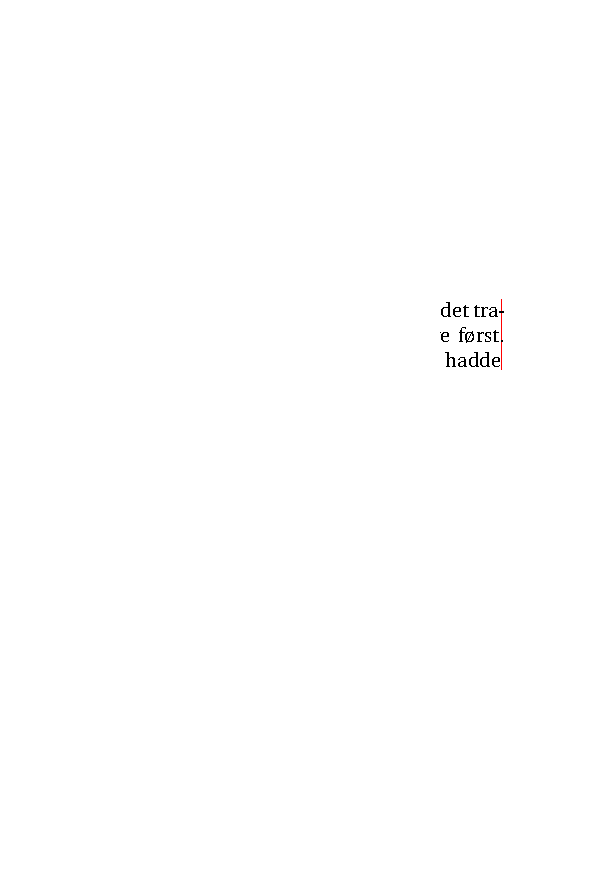
\includegraphics[width=\marginparwidth]{content/examples/hanging-punctuation/hanging-punctuation-crop.pdf}
    \captionof{figure}[Hengende punktuering]{Eksempel på hengende punktuering. Satt med \LaTeX{} og pakken microtype.}
    \label{fig:hanging-punctuation}
}

For å oppnå det andre målet om jevn farge i tekstene sine var det viktig for Gutenberg å få mest mulig uniform avstand mellom ordene i teksten. Det er vanlig når man setter en tekst at man har fastsatt et visst maks- og minimumsmål for tillatt avstand mellom ord, slik at man har noe spillerom å jobbe med når man skal justere teksten. Men ikke alltid gir dette nok rom, og man trenger andre metoder. Gutenberg gjorde dette ved å skape flere varianter av samme glyph. Typisk da kunne for eksempel en enkelt bokstav «e» ha flere varianter i forskjellige bredder som kunne erstattes for å gi mer spillerom til å justere avstanden mellom ordene. Gutenberg utviklet rundt 290 forskjellige bokstavtyper som han brukte i sin tekstsetting. Videre vet vi også at orddeling selvfølgelig også er et viktig redksap i å oppnå mest mulig jevn farge.

Selv i dag regnes Gutenbergs 42-linjersbibel som en standard for høykvalitets boktrykk, og flere av de typografiske teknikkene han utviklet er ennå ikke å se i dagens komersielle produkter \cite{thanh2000microtypographic}.


\section{Typografen erstattes av datamaskiner}

Da datamaskinene ble tilstrekkelig kraftig var det naturlig at man ønsket at de tok seg av mye av det typografiske arbeidet. Det ville føre kostnader ned og effektiviteten opp. Enkelte av disse typografiske oppgavene er aspekter som maskiner er mye flinkere enn mennesker til å utføre; for eksempel justering av tekst for å få mest mulig uniforme avstander mellom ord. Et slikt problem kan reduseres til en matematisk funksjon som vekter hver mulige løsning og vi kan da be maskinen om å optimalisere over denne funksjonen. Donald Knuth viser også i sin artikkel \textit{Breaking Paragraphs into Lines*} \cite{knuth1981breaking} at vi nå også kan se på hele avsnitt av gangen når vi skal utføre denne optimaliseringen, i stedet for å bare se på en linje av gangen, som var vanlig når dette arbeidet ble gjort for hånd, eller med de tidligere eksisterende algoritmene.

Et problem som viste seg å være ganske vanskelig for datamaskiner er automatisk deling av ord ved linjeskift, som ikke er løst helt selv i dag. Dette er en svært kompleks lingvistisk operasjon, men for et menneske kan denne oppgaven virke ganske triviell. Vi kjenner til innholdet og betydningen av settningen hvor ordet oppstår og vi har en viss forståelse for reglene som ligger til grunn for orddeling i det språket vi uttrykker oss i. Slik finner vi ganske enkelt rett delepunkt. Men for datamaskiner er det en helt annet kompleksitet. Datamaskiner vil typisk ikke kjenne til den semantiske betydningen av et ord; og for eksempel deling mellom to komponenter i et sammensatt ord blir vanskelig. Det vil også oppstå problemer ved deling av \textit{homonymer}. \sidenote{Homonymer er ord som uttales eller skrives likt.} I slike tilfeller vil konteksten som ordet opptrer bestemme hvordan det skal deles korrekt. For eksempel ordet snekker skal deles som snek-ker (når vi mener håndtverkeren) og snek-k-er (når vi mener båten).

Tekster med lange linjer og kun én kolonne vil typisk ha mindre problemer med å justere teksten og ha færre tilfeller av orddeling ved linjeskift. Derimot tekster hvor det er vanlig med smalere kolonner, som avisartikler, vil dette være et mye mer fremtredene problem. Man får få ord på en linje og får da tilsvarende mindre totalt spillerom i avstanden mellom ordene å jobbe med når teksten skal justeres. Ordene må oftere deles. For å demonstrere problemet ved dette har jeg satt opp tre eksempler som illustrerer dette i figur \ref{fig:three-columns}. 

\begin{SCfigure}
\fcolorbox{red}{white}{
  \parbox{0.27\textwidth}{
  \hyphenpenalty = -1000
 \looseness=-10000
  \spaceskip .5em plus .25em minus .25em
  %\tolerance = -1
  Det var en gang en konge som hadde en datter, og hun var så vakker at hun var navngjeten både vidt og bredt; men hun var så alvorlig av seg at hun aldri kunne le, og så var hun så stor på det at hun sa nei til alle som kom og fridde til henne, og ikke ville hun ha noen, om de var aldri så gilde, enten det var prinser eller herremenn. Kongen var lei av dette for lenge siden, og syntes at hun kunne gifte seg, hun som de andre …
  }
}%
%
\hskip 1em
\fcolorbox{red}{white}{
  \parbox{0.27\textwidth}{
  \hyphenpenalty = 10000
  \looseness=-1
  \spaceskip .5em plus 2em minus .3em
  \tolerance = -1
  Det var en gang en konge som hadde en datter, og hun var så vakker at hun var navngjeten både vidt og bredt; men hun var så alvorlig av seg at hun aldri kunne le, og så var hun så stor på det at hun sa nei til alle som kom og fridde til henne, og ikke ville hun ha noen, om de var aldri så gilde, enten det var prinser eller herremenn. Kongen var lei av dette for lenge siden, og syntes at hun kunne gifte seg, hun som de andre …
  }
}%
%
\hskip 1em
\fcolorbox{red}{white}{
  \parbox{0.27\textwidth}{
  \hyphenpenalty = 10000
  \looseness=-1
  \spaceskip .5em plus .5em minus .15em
  \tolerance = -1
  Det var en gang en konge som hadde en datter, og hun var så vakker at hun var navngjeten både vidt og bredt; men hun var så alvorlig av seg at hun aldri kunne le, og så var hun så stor på det at hun sa nei til alle som kom og fridde til henne, og ikke ville hun ha noen, om de var aldri så gilde, enten det var prinser eller herremenn. Kongen var lei av dette for lenge siden, og syntes at hun kunne gifte seg, hun som de andre …
  }
}

\label{fig:three-columns}
\caption[Eksemepler på tekstsetting av smale kolonner]{Første kolonne viser en spalte med tillatt orddeling og noe rom for justering av mellomrom mellom ord. Andre kolonne tillater justering mellom ord, men ingen orddeling. I siste kolonne er også justeringsmulighetene tatt bort. Alle kolonnene er typsatt med med \TeX{}.}
\end{SCfigure}

Siste eksempel er typesatt uten tillatt orddeling og med minimale justeringsmuligheter mellom ordene. Denne teksten ser vi får en fin og jevn farge over seg, men den klarer rett og slett ikke å plassere ordene innenfor den satte rammen med disse strenge kravene, og enkelte ord vil gå utenfor rammen. Ved eksempel to har justeringsmulighetene mellom ordene blitt økt betraktelig. Dette fører til at vi får rette marger, men vi ser fargen i teksten blir ganske ujevn. Det blir flere hvite tomrom i teksten som ikke ser spesielt vakkert ut og kan virke distraherende. Et annet relatert problem som lettere oppstår med løs justering er såkalte \textit{elver} eller \textit{fosser}. \sidenote{Elver og fosser er betegnelsen på hvite tomrom som går vertikalt over flere linjer i teksten. Eksempelvis ser vi dette i figur \ref{fig:three-columns} i midten av andre kolonne.} I første eksempel tillater vi stor grad av orddeling, men med et begrenset spillerom for justering av avstanden mellom ordene. Her får vi både rette marger og en fin farge over teksten.

For å kunne oppnå god typografi i tekster, spesielt i smale kolonner, er det viktig at en algoritme for automatisk orddeling i størst mulig grad finner alle mulige delepunkter i et ord, for å videre kunne gi algortimen som skal dele paragrafer inn i linjer mest mulig å jobbe med. I denne oppgaven vil jeg først se på hvordan algoritmer typisk løser problemet med automatisk orddeling, se i hvor stor grad disse finner delepunkter i ord (og hvor mange feiltreff de har), for så se om det er mulig å utvikle noe som løser dette på en bedre måte — for å igjen kunne sette tekst bedre.

\section{Oppgavens struktur}

Første del av oppgaven tar for seg orddanning og orddeling: I kapittel to ser vi på ordanning -- hvordan ord er bygget opp, hvordan vi setter dem sammen for å danne nye ord og hvordan vi klassifiserer dem i ordklasser. Dette er relevant for orddelingsreglene. Kapittel tre ser på reglene for orddeling på norsk. I kapittel fire presenteres ulike metoder for automatisk orddeling. Femte kapittel gir en oversikt over tidligere arbeid i fagfelte, både orddelingsalgoritmer og algoritmer for deling av sammensatte ord. Til sist beskrives ressurser som benyttes i del to av oppgaven.

Andre del er en beskrivelse av arbeidet med å utvikle en regelbasert orddeler: Syvende kapittel beskriver arkitektur og implementasjon av en regelbasert orddeler, mens kapittel åtte viser resultater fra testingen av orddeleren samt en diskusjon rundt resultatene.

Tredje og siste del er en oppsummering av oppgaven: I niende og siste kapittel konkluderes oppgaven med en tilbakeblikk på hva vi har lært underveis og et blikk på hvilke muligheter det er for videre arbeid.

	\part{Orddanning og orddeling}
	\chapter{Orddanning}
\label{sec:orddanning}

For å få en god forståelse for de norske reglene for orddeling er det nødvendig med en forståelse for orddanning (hvordan ord bygges opp) og noe om ordklasser (grupper vi deler ordene inn i). Norsk Referansegrammatikk \cite{faarlund1997norsk} gir en god innføring i disse temaene og jeg vil gjengi noe av det innholdet her. I følge Wikipedia \cite{wiki-nrg} er denne grammatikken «i praksis det sentrale referanseverket når det gjeld norsk grammatikk».

\begin{center}
{\huge\color{gray!50}{\decofourleft}}
\end{center}

I norsk kan vi ha \term{komplekse ord} og \term{enkle ord} -- ord som ikke kan deles opp i mindre deler. Disse ordene kaller vi for \term{rotord}. 

\ex{hus, hage, båt}

Av disse rotordene har vi muligheter til å danne nye ord gjennom \textit{bøyning}, \textit{avledning}, \textit{sammensetning}; eller kombinasjoner av disse (se figur \ref{fig:ordtre}). 
\marginelement[-7]{
\tikzset{
  treenode/.style = {align=center, inner sep=0pt, text centered},
  arn_n/.style = {treenode},% arbre rouge noir, noeud noir
  arn_r/.style = {treenode, red},% arbre rouge noir, noeud rouge
}
\begin{tikzpicture}[->,>=stealth',level/.style={sibling distance = 2.4cm/#1,
  level distance = 1.1cm,   text height=1.5ex,
    text depth=.25ex},font=\footnotesize\sffamily] 
\node [arn_r] {umuligheten}
    child{ node [arn_n] {stamme} 
            child{ node [arn_n] {prefiks} 
							child{ node (1) [arn_r] {u}}
            }
            child{ node [arn_n] {rot}
							child{ node (2) [arn_r] {mulig}}
            } 
            child{ node [arn_n] {avledning}
							child{ node (3) [arn_r] {het}}
            } 
    }
    child{ node [arn_n] {bøyningsendelse}
            child{ node [arn_r, below=2.7em] {en} }
		}
; 
\end{tikzpicture}
    \captionof{figure}[Eksempel på orddanning]{Trestruktur som viser hvordan ord dannes gjennom avledningsaffikser og bøyningsendelser.}
    \label{fig:ordtre}
}
Når vi kombinerer disse til å danne nye ord gjøres det trinnvis i en ikke-tilfeldig rekkefølge, da rekkefølgen vil ha betydning på det nye ordet som dannes. Hvis vi sammenligner ordene rødvinsglass og krystallvinglass ser vi betydningen av dette. Vi antar at rødvinsglass er satt sammen av rødvin og glass, som betyr «glass for rødvin», mens derimot krystallvinglass er satt sammen av ordene krystall og vinglass som betyr «vinglass av krystall» (se figur \ref{fig:rodvin} og \ref{fig:krystall}).

\marginelement[-0.5]{
\tikzset{
  treenode/.style = {align=center, inner sep=0pt, text centered},
  arn_n/.style = {treenode},% arbre rouge noir, noeud noir
  arn_r/.style = {treenode, red},% arbre rouge noir, noeud rouge
}
\begin{tikzpicture}[->,>=stealth',level/.style={sibling distance = 2.4cm/#1,
  level distance = 1.1cm,   text height=1.5ex,
    text depth=.25ex},font=\footnotesize\sffamily] 
\node [arn_r] {rødvinsglass}
    child{ node [arn_r] {rødvins} 
            child{ node [arn_r] {rød} 
            }
            child{ node (1) [arn_r] {vins}
            } 
    }
    child{ node [arn_r, right of = 1,xshift=1cm] {glass}
		}
; 
\end{tikzpicture}
    \captionof{figure}[Syntakstre for «rødvinsglass»]{Syntakstre som viser hvordan ordet «rødvinsglass» er satt sammen.}
    \label{fig:rodvin}
}

\marginelement[9]{
\tikzset{
  treenode/.style = {align=center, inner sep=0pt, text centered},
  arn_n/.style = {treenode},% arbre rouge noir, noeud noir
  arn_r/.style = {treenode, red},% arbre rouge noir, noeud rouge
}
\begin{tikzpicture}[->,>=stealth',level/.style={sibling distance = 2.4cm/#1,
  level distance = 1.1cm,   text height=1.5ex,
    text depth=.25ex},font=\footnotesize\sffamily] 
\node [arn_r] {krystallvinglass}
    child{ node [arn_r, left of = 1,xshift=0.5cm] {krystall}
		}
    child{ node [arn_r] {vinglass} 
            child{ node (1) [arn_r] {vin} 
            }
            child{ node [arn_r] {glass}
            } 
    }
; 
\end{tikzpicture}
    \captionof{figure}[Syntakstre for «krystallvinglass»]{Syntakstre som viser hvordan ordet «krystallvinglass» er satt sammen.}
    \label{fig:krystall}
}

Videre i denne teksten vil jeg først beskrive de relevante ordklassene, før vi ser på orddanning gjennom bøyninger, avledninger og sammensetninger.

\clearpage
\section{Ordklasser}
\label{sec:ordklasser}

\term{Leksemer}\sidenote{I følge Wikipedia er et leksem «et abstrakt begrep innenfor språkvitenskapen som viser til alle ord som er forskjellige former av et bestemt ord.» \cite{wiki-leksem} Eksempelvis er bil, bilen, bilene og biler ett leksem.} har ulik form og funksjon, som gjør at vi kan dele dem inn i forskjellige \term{ordklasser}. Ordklassene gjør det mulig å kunne beskrive grupper av ord på en generell basis, for igjen å kunne gi gramamtiske regler basert på dette. Tre kriterier ligger til grunne for å danne grunnlaget for ordlassene: morfologiske (går på hvilke affiks ordene kan få, spesielt bøyningsendelsen), syntaktiske (funksjonen ordet har i setningen) og semantiske (skiller blant annet mellom leksikalse ord, grammatiske ord og pro-ord). Norsk referansegrammatik som ligger til grunne for denne teksten har en ordklasseinndeling som avviker noe fra den tradisjonelle inndelingen\cite{faarlund1997norsk}:

\begin{quote}
… den tradisjonelle inndelinga er basert på ulike kriterer og skaper ofte problemer i språkbeskrivelsen. Her skal vi sette opp en ordklasseinndeling ut fra helhetlige inndelingskriterier, men likevel slik at den ikke bryter mer enn nødvendig med den tradisjonelle inndelinga.
\end{quote}

I Norsk referansegramatikk benyttes de morfologiske, altså bøyningen,  som kriterie for ordklasseinndelingen. Ved andre nivå benyttes syntaktiske kriterier. I denne oppgaven er jeg kun interessert i ordklassene som legger morfologiske kriterier til grunne, altså \term{ord med bøyning}. Det er ordklassene substantiv, verb, adjektiver, pronomen og determinativ.  Av disse er vi i oppgavens sammenheng kun interessert i ord(under)klasser som har den syntaktisk egenskap \textit{leksikalske}. Da sitter vi i gjen med ordklassene \term{substantiv} (utelatt proprium som står ubøyd), \term{verb} og \term{adjektiv} (utelatt ordenstall som står ubøyd).

\subsection{Ordklasseinndeling}

\paragraph{Substantiv} Typisk navn og betegnelser på gjenstander, idivider og abstrakte begreper.
	\begin{itemize}
		\item Morfologisk kriterium: Bestemt artikkel.
		
		\ex{\textit{bil} -- \textit{bilen}}{}
		
		\item De fleste har også tallbøning.
		
		\ex{\textit{bil} -- \textit{biler}}{}
		
	\end{itemize}
\paragraph{Verb} Betegner ofte en handling, prosess eller tilstand.
	\begin{itemize}
		\item Morfologisk kriterium: Tempusbøyning.

		\ex{\textit{kaster} -- \textit{kastet}}{}
		
		\item I tillegg til finitt (presens og preteritum) har verb også infinitt (infitiv og partisipp). 
	\end{itemize}
	
\paragraph{Adjektiv} Først og fremst ord som kan gradbøyes, altså får lagt til (e)ere eller (e)st, med eller uten vokalveksling.
	\begin{itemize}
		\item Morfologisk kriterium: Gradbøyning.
		
		\ex{\textit{fin} -- \textit{finere} -- \textit{finest}}{}\newline
		\exx{\textit{stor} -- \textit{større} -- \textit{størst}(vokalveksling)}{}
		
		\item Bøyes også i genus, tall og bestemthet.
	\end{itemize}

\section{Avledninger}

En \term{avledning}
\sidetable[Liste over avledningsprefikser]{%
	Avledningsprefikser hentet fra Norsk referansegrammatikk \cite{wiki-nrg}. Tegnforklaring: \textbf{N} (Norske), \textbf{G} (Germanske) og \textbf{F} (Fremmedspråklige). Hentet fra Norsk Referansegrammatikk \cite{wiki-nrg}.
  \label{table:prefikser}}{%

\begin{tabularx}{\marginparwidth}{lp{0.7\marginparwidth}}
\toprule
\multicolumn{2}{c}{\textbf{Prefikser}}                                                                                                                                                                                                                                                                                                                                                                                                                                \\ \midrule
\multicolumn{1}{l}{\textbf{N}}    & \multicolumn{1}{l}{u, mis, van, be, for, fore, føre}                                                                                                                                                                                                                                                                                                                                                           \\ 
\multicolumn{1}{l}{\textbf{G}} & \multicolumn{1}{l}{an, bi, er, ge, unn}                                                                                                                                                                                                                                                                                                                                                                        \\
\textbf{F}                & a, ad, an, andro, ante, anti, antro, bi, bio, centi, de, des, di, dia, dis, dys, eks, erke, eu, ev, geo, giga, hetero, homo, hyper, hypo, il, im, in, inter, intra, iso, ko, kon, kontra, kvasi, makro, maksi, mega, meta, midi, mikro, milli, mini, mono, multi, non, orto, pan, para, poly, post, pre, pro, proto, pseudo, psevdo, re, retro, semi, sub, super, syn, tele, trans, ultra, uni, vara, vise, øko \\ \bottomrule
\end{tabularx}
}
 er ord som dannes ved hjelp av avledningsaffikser\footnote{Et affiks er en orddel som føyes til en rot eller stamme. Kan gi videre avledninger og bøyninger, og deles videre inn i \textit{prefiks}, \textit{innfiks} og \textit{suffiks}.} enten som prefikser hvor et affiks tilføres foran ordstammen (se tabell \ref{table:prefikser} for liste over ofte brukte prefikser).

\ex{\textit{mis}forstå}


Eller som et suffiks hvor affikset tilføres enden av ordstammen (se tabell \ref{table:suffikser} for ofte brukte suffikser).

\ex{kjær\textit{lig}}

\sidetable[Liste over norske avledningssuffikser]{%
	Norske avledningssuffikser hentet fra Norsk referansegrammatikk \cite{wiki-nrg}.
  \label{table:suffikser}}{%

\begin{tabularx}{\marginparwidth}{p{0.9\marginparwidth}}
\toprule
\multicolumn{1}{c}{\textbf{Suffikser}}                                                                                                                                                                                                                                                                                                                                                                                                                                \\ \midrule
ing, ning, ling, else, sel, nad, sjon, er, ar, dom, skap, het, itet \\ \bottomrule
\end{tabularx}
}

Avledninger i norsk språk er det vi vil kalle for \term{produktive}. Måten vi danner ord på er produktiv når nye ord kan dannes på samme måte. For eksempel kan vi alltids lage substantiver av verb ved å påføre suffikset \textit{-ing}. Slik kan vi alltid lage nye ord av verb som kommer inn i det norske språket.

\ex{skuldersurf\textit{ing}}

Vi kan også danne ord ved avledning ved å tilføre avledningssuffikset -het til adjektiv og danne nye substantiv.

\ex{god\textit{het}}

\section{Bøyninger}

Når et ord bøyes får det et tillagt betydningselement, stort sett ved tillegg av bøyningsendelser (suffiks). Eksempelvis \textit{båt} -- \textit{båter}. Eller ved såkalt indre bøyning, også kalt vokalskifte. Eksempelvis \textit{mann} -- \textit{menn}. Norsk referansegrammtikk \cite{faarlund1997norsk} nevner åtte forskjellige bøyningskategorier: \textit{genus} (kjønn), \textit{tall} (numerus), \textit{bestemthet}, \textit{kasus}, \textit{grad}, \textit{tempus}, \textit{modus} og \textit{diatese}. I denne sammenhengen her er vi kun avhengig av bøyningskategoriene som gjelder for ordklassene substantiv, verb, og adjektiv --- alltså genus, bestemthet, tall, tempus, og grad (se kapittel \ref{sec:ordklasser} for beskrivelse av ordklassene).


\paragraph{Genus} Tre vanlige kjønn, ord fra visse ordklasser bøyes forskjellige etter hvilke ordklasser de hører til: \term{maskulin} (hannkjønn), \term{feminum} (hunnkjønn) eller \term{nøytrum} (intentkjønn).

\paragraph{Tall} Uttrykker tallforhold gjennom bøyninger og bøyes i entall og flertall.

\ex{båt}{(entall)}\newline
\exx{båt\textit{er}}{(flertall)}\newline

\paragraph{Bestemthet} Skiller mellom enheter som er spesifikke og identifiserbare (bestemt) eller de som ikke er det (ubestemt) \cite{wiki-bestemthet}. Kan uttrykkes på flere måter, spesielt viktig her, etterhengt \term{bestemt artikkel}:

\ex{gutt}{(ubestemt)}\newline
\exx{gutt\textit{en}}{(bestemt)}\newline

Bestemt artikkel endrer seg i genus og tall etter ordet.

\ex{båt\textit{en}}{(mask. ent.)}\newline
\exx{båt\textit{ene}}{(best. flert.)}\newline

\paragraph{Grad} En sammenlignen, komperasjon, av subjekter. Bøyes i tre grader: \textit{positiv}, \textit{komperativ} og \textit{superlativ}.

\ex{fin}{(grunform)}\newline
\exx{fin\textit{ere}}{(komperativ)}\newline
\exx{fin\textit{est}}{(superlativ)}

\paragraph{Tempus} Angir tidspunkt for handlingen eller tilstanden som vises til, og bøyes i \term{presens} og \term{preteritum}.

\ex{hør\textit{er}}{(presens)}\newline
\exx{hør\textit{te}}{(preteritum)}\newline

\section{Ordsammensettning}

En ordsammensetning er en sammenstilling av to ord for å danne et nytt. Disse kan være mer eller mindre \term{gjennomskuelige} eller mer eller mindre \term{leksikaliserte}. Gjennomskuelige sammensetninger er ord vi intutivt kan forstå betydningen av uavhengig om vi har sett dem tidligere. De leksikaliserte sammensetningene er orddanninger vi ikke forstår intuitivt som gjerne er konstruert mer metaforiske.

\ex{vinter+dag}{(gjennomskuelig)}\newline
\exx{danse+løve}{(leksikalisert)}

En sammensetning er satt sammen av ord som alle bør kunne opptre på egenhånd som egne ord. Dermed vil \texttt{eple+kake} være et sammensatt ord, men ikke \textit{pult+ost}. Selv om «pult» kan ha flere betydninger i norsk, er det ingen av disse som refereres til i denne sammenhengen\sidenote{I følge Norsk etymologisk ordbok kommer ordet «pult» fra middelalderlatinordet «pulta» som betyr grøt eller velling. \cite{de2013norsk} Men ikke et ord som står oppført i ordboka alene med denne definisjonen.}. Det er altså ikke et ord som har egen betydning når det står alene. 

En sammensetning vil bestå av først et forledd, som oftest står ubøyd, og så et etterledd, som stort sett bestemmer ordklassen.

\ex{kryp+inn}{(=subst., inn=prep.)}

Forleddet i sammensetningen kan igjen være sammensatt av flere ledd. Det kan altså bestå av flere rotord.

\ex{[flyve+maskin]+instruktør}

Punktet der forleddet og etterleddet treffer hverandre kalles for \term{sammensetningsfugen}. Den vanligste formen for fuge er en nullfuge, der forledd og etterledd settes sammen uendret. Men i en del tilfeller oppstår det fuge-s eller fuge-e (og i mer sjeldene tilfeller andre bindebokstaver eller bindeord), som binder leddene sammen. 

\section{Bindebokstaver}
\label{sec:fuge-bokstav}

Det finnes flere typer bindeelementer som binder sammen forledd og etterledd og som tydligere kan vise hva som er hovedgrensen i ordet. Vanligste bindingen er nullfuge, hvor begge ledd har samme form som grunnform.

\ex{båt+hus}{(nullfuge)}

Ifølge Munthe (1972, i Johannesen og Hauglins artikkel «An automatic analysis of Norwegian compounds» \cite{johannessen1996automatic}) er 10,4 \% av alle ord i norske tekster sammensatte. Av disse har omtrent 75 \% av sammensatte ord nullfuge; hvor leddene er satt sammen uten en bindebokstav \cite{johannessen1996automatic}. Det betyr at rundt 25 \% av alle sammensatte ord i norsk inneholder en bindebokstav. Av bindebokstaver har vi de vanligste: \textit{-s} og \textit{-e}. Noe mer sjeldent ser vi: \textit{-en}, \textit{-a}, \textit{-er} og \textit{-es}. I svært få tilfeller kan det oppstå: \textit{-o} og \textit{-ium → -ie} \cite{faarlund1997norsk,bindebokstaver}.

\ex{vindu\textit{s}vask}{(-s)}\newline
\exx{jule\textit{e}kveld}{(-e)}\newline
\exx{hit\textit{en}for}{(-en)}\newline
\exx{ås\textit{a}tro}{(-a)}\newline
\exx{student\textit{er}samfunn}{(-er)}\newline
\exx{makt\textit{es}løs}{(-es)}\newline
\exx{afr\textit{o}amerikansk}{(-o)}\newline
\exx{labrator\textit{ie}forsøk}{(-ium → -ie)}\newline

\begin{center}
{\huge\color{gray!50}{\decofourleft}}
\end{center}

Norsk referansegramatikk nevner at binde-s og binde-e er de desidert mest frekvente av bindebokstavene (se kapittel~\ref{sec:fuge-frekvens} for en ytterligere analyse av frekvensen). Derfor vil jeg gi en nærmere beskrivelse av spesielt disse to i de følgende kapitlene. 

\subsection{Binde-s}
\label{sec:ord-bind1}

Det finnes ingen klare regler for binde-s og når den skal tilføres  sammensetningsfugen, men det finnes noen rettledene punkter. Det er en viss taleforskjell å spore. Ved sammensetninger uten binde-s og et forledd som er et enstavelsessubstantiv ser vi noramlt får tonem\sidenote{Tonem er en betydningsdifferensierende tonegang («musikk») ved uttale av ord som gjør at vi kan skille dem. Det er mange ord som kun kan skilles gjennom tonemet, ord som er homografe, men som ikke er homonyme -- for eksempel ordet snekker. Vi har \textit{(en) snekker} (håndtverkeren) og \textit{(flere) snekker} (båten), hvor de henholdsvis har tonem én og tonem to.} to (\textit{bønner} -- erteblomsten). Sammensetninger med binde-s uttales helst med tonem én (\textit{bønner} -- religiøs praksis) når forleddet er enstavet. Når forleddet er to eller flerstavet får sammensetningen samme tonem som forleddet.

Norsk referansegrammatikk \cite{faarlund1997norsk} lister også opp en rekke andre karakteristikker ved binde-s, som jeg vil gjengi her.

\begin{items}
	\item Forleddet er et rotord …
	\begin{itemize}
		\item … og forleddet ender på \textit{-s}, \textit{-sj} eller en konsonantgruppe som har lik lyd, gir ingen binde-s.
		
		\ex{løs+katt}{}
		
		\item … og forleddet ender på en vokal, gir sjeldent binde-s, spesielt når forleddet er enstavet.
		
		\ex{le+skur}{}
		
		\item … og forleddet ender på konsonant, gir binde-s i en god del tilfeller, men det er fortsatt vanligere uten binde-s. Binde-s er spesielt sjeldent etter trykklett \textit{en}, \textit{el}, \textit{er} eller ord på \textit{ft}, \textit{kt} og \textit{m}.
		
		\ex{vakt+avløsning}{}
		
	\end{itemize}
	
	\item Når forleddet er en avledning …
	\begin{itemize}
		\item … og forleddet er prefiksavledet, gir en tendens til binde-s, spesielt ved prefiksene \textit{an}, \textit{be}, \textit{bi} og \textit{for(e)}.
		
			\ex{forslag\textit{s}+kasse}{}
		
		\item … og forleddet er suffiksavledet, gjør det vanlig med binde-s, spesielt etter nordiske suffikser som \textit{(n)ing}, \textit{dom}, \textit{else}, \textit{het}, \textit{leik}, \textit{nad}, \textit{sel} eller \textit{skap}.
		
		\ex{anretning\textit{s}+rom}{}
		
		\item … og forleddet er suffiksavledet av fremmed suffiks, gjør binde-s ganske vanlig. 
		
		\ex{plenum\textit{s}+forelesning}
		
		\item … og forleddet er et verbalsubstantiv (uten suffiks), gjør det vanlig med binde-s. 
		
		\ex{hørsel\textit{s}+vern}{}
	\end{itemize}
	
	\item Når forleddet er en sammensetning …
	\begin{itemize}
		\item … gir det i større grad binde-s enn når forleddet er et rotord.
	
		\ex{vin+glass}{}\newline
		\exx{rødvin\textit{s}+glass}{}
		
		\item … og ender på vokal gir det sjeldent binde-s.
		
		\ex{bispedømme+råd}{}
		
		\item … og forleddet ender på \textit{en}, \textit{el} eller \textit{er} får man normalt ikke binde-s. Untaktet er de som ender på \textit{-sel}.
		
		\ex{næringsmiddel+industri}{}\newline
		\exx{anførsel\textit{s}+tegn}{}
		
	\end{itemize}
\end{items}

\subsection{Binde-e}
\label{sec:ord-bind2}

Binde-e forekommer også relativt ofte, men ikke like hyppig som fuge-s. Det finnes heller ingen veldig klare regler for binde-e, men vi har igjen noen karakteristikker \cite{faarlund1997norsk}.

\begin{items}
	\item Binde-e forekommer ofte når forleddet er et enstavet substantiv som ender på konsonant. 
		
		\ex{jule+kake}{}
		
	\item Binde-e forekommer sjeldnere foran etterledd på vokal.

	 \ex{jul+aften (men jule+kveld)}{}
	 
	\item Når forleddet er sammensetning, er binde-e sjelden. 
	 
	\ex{storsild+fiske (men sild\textit{e}+fiske)}{}

	\item Ved forledd som er substantiv og ender på trykklett \textit{-e}, hører \textit{e}-en med til forleddet og regnes ikke som en binde-e. 

	\ex{jente+barn}{}	
\end{items}


\subsection{Regler for bindebokstaver}
\label{sec:reg-bind}

Bruk av bindebokstaver er vanskelig. Det finnes ingen absolutt regelbruk for dette. Norsk referansegrammatikk \cite{faarlund1997norsk} gir noen regler for hvordan disse brukes og opptrer i det norske språk, men er noe ufullstendig. Janne Bondi Johannessen og Helge Hauglin gir noen ytterligere rettningslinjer for analyse av binde-s og binde-e i sammensatte ord i norsk språk. Disse retningslinjene vil være til stor nytte i algoritmen for å dele ord, og jeg vil raskt gjengi disse her\cite{johannessen1996automatic}:

\begin{enum}
	\item Tolk sammensetningen som en kombinasjon av to rotord, uten fuge om mulig.
	
		\ex{løve-manke}{}\newline
		\exx{Ikke: løv-e-manke}{}
	
	\item Tolkning som binde-s er foretrukket om det er en tvetydig tolkning der s-en også kan ingå som første bokstav i et verbalt etterledd.
	
		\ex{aluminium-s-nakke}{}\newline
		\exx{Ikke: aluminium-snakke}{}
	
	\item Tolkning som binde-s er foretrukket fremfor nullfuge om forleddet i seg selv er et sammensatt ord.
	
		\ex{lesesal-s-turer}{}\newline
		\exx{Ikke: lesesal-sturer}{}
	
	\item Binde-s kan aldri følge binde-e og visa versa.
		
		\ex{hest-e-sal}{}\newline
		\exx{Ikke: hest-e-s-al}{}
	
	\item Ved to analyser som gir likt antall medlemmer og ingen bindebokstav er involvert, velg, hvis mulig, analysen som er et substantiv.
		
		\ex{hun-dyr}{(S)}\newline
		\exx{Ikke: hund-yr}{(V)}
	
	\item Ved to like analyser med tanke på bindebokstav og regelen over, og en av dem har et forledd som i seg selv er et sammensatt ord, velg den.
		
		\ex{fagplan-arbeid}{}\newline
		\exx{Ikke: fag-planarbeid}{}
	
	\item Binde-e kan kun settes sammen med en stamme som har enkelt stavelse.
		
		\ex{hest-e-ekvipasje}{}\newline
		\exx{tre-hest-ekvipasje}{}\newline
		\exx{Ikke: tre-hest-e-ekvipasje}{}
	
	\item Stammer kan komme før forleddet før -e så lenge de ikke danner sammensetning med forleddet.
		
		\ex{konge-hus-hest-e-ekvipasje}{}\newline
		\exx{Ikke: konge-hus-hest-ekvipasje}{}
	
	\item Binde-s opptrer ikke etter en konsonantsekvens med sibilanter … 
		
		\ex{busk-spilling}{}\newline
		\exx{Ikke: busk-s-pilling}{}
	
	\item … med mindre forleddet er sammensatt.
		
		\ex{enebærbusk-spilling}{}\newline
		\exx{enebærbusk-s-pilling}{}
	
	\item Hvis forleddet er ukjent, velg analysen med det lengste etterleddet.
		
		\ex{Ibsen-stykket}{}\newline
		\exx{Ikke: Ibsens-tykke}{}
	
\end{enum}


	\chapter{Orddeling}
\label{sec:orddeling}

Orddeling ved linjeskift i det norske språk er regelbasert (i motsats til for eksempel amerikansk-engelsk som er uttalebasert). Det er Språkrådet som er ansvaret for å sette rettningslinjer og klargjøre hva som er korrekte gjeldende regler for orddeling. Dette mandatet fikk de etter Stortingsmelding nr. 100. Språkrådet har i paragraf 3 av sine vedtekter fått følgende rolle:

\begin{quote}
Språkrådet gir råd og rettleiing om tekniske skrivereglar og skal så langt det er tenleg, klargjera kva reglar som er obligatoriske for korrekt språk.
\end{quote}

Reglene for orddeling er en del av det som kalles tekniske skriveregler, som er utviklet over flere år fra mange kilder. Forskjellige komitéarbeid hvor blant annet språkprofessor Finn-Erik Vinje har vært delaktig, standardiseringsarbeid og annet.\cite{Simonsen2015} Disse reglene ble gjort gjeldene i 1973 og først publisert i Finn-Erik Vinjes bok Skriveregler. 

\section{Reglene}
\label{sec:orddelingsreglene}

Norsk rettskrivning benytter seg av to hovedregler for orddeling, \textit{ordleddsregelen} og \textit{enkonsonantregelen}, samt kravet om at det alltid skal være minst én vokal per linje. Disse er enkle å forstå, men problemene oppstår ved alle unntakene og tvedydighetene man må forholde seg til. Reglene kan kort oppsummeres slik:

\begin{description}
	\item[Ordleddsregelen] Del ord mellom betydningsbærendebærende og/eller lett gjenkjennelige orddeler.
	\item[Enkonsonantregelen] Uavhengig av ordets betydning, la én konsonant følge med til neste linje.
\end{description}

I mange tilfeller kan man velge fritt mellom reglene. Det viktigste prinsippet er å ungå komiske, forvirrende eller meningsendrende ordbilder. Videre i teksten vil jeg forklare reglene og deres unntak i mer detalj. Innholdet i denne teksten er basert på skriveriene til Finn-Erik Vinje i boken Skriveregler \cite{vinje}.

\subsection{Ord og uttrykk som ikke skal deles}

Vi skal ikke dele følgende ord og uttrykk: 
\begin{inparaenum}[\itshape a\upshape)]
\item Enstavelsesord, 
\item forkortelser,
\item  årstall, datoer og andre sammenhengende siffer- eller tegngrupper, og
\item forbindelser av ordenstall i numerisk form og tilhørende substantiv
\end{inparaenum}.

	\ex{kai, dag, skjær}{(a)}\newline
	\exx{ADHD}{(b)}\newline
	\exx{1988, 299 792 458 m/s}{(c)}\newline
	\exx{14. september}{(d)}

\subsection{Unntak fra enkonsonantregelen}
\label{sec:enkons-untak}

Følgende forbindelser deles ikke når de gjengir én og samme lyd og tilhører samme stavelse:	\textit{dh, gh, gj, kj, sc, sch, sh, sj, skj, sk}. Delepunktet settes foran forbindelsene.

	\ex{kan-skje}{}

\subsection{Usammensatte ord}

Ord med to eller flere stavelser, som ikke er sammensatt, eller som opfattes som usammensatte, deles etter enkonsonantregelen. Det er også lov å dele mellom vokaler hvis de hører til hver sin stavelse.

	\ex{hø-re}{}\newline
	\exx{are-al}{}

\subsection{Sammensatte ord}

Sammensatte ord deles etter ordleddsreglen. Ved eventuell komposisjonsfuge tilhører fugen første leddet av sammensetningen. Ved sammensatte ord som består av flere enn to ordkomponenter så \textit{bør}\footnote{Finn-Erik Vinje bruker selv ordet bør i Skriveregler\cite{vinje}, som betyr at dette er en anbefaling, men ikke et krav!} de deles i hovedgrensen. Også ukjente og fremmede sammensetninger kan deles i sammensetningen. Hvis leddene ikke kan regnes for å være lett gjenkjennelige er det lov å dele etter enkonsonantsregelen. I enkelte tilfeller kan det være nødvendig eller ønskelig å dele sammensatte ord i ett av rotordene. Da benytter man seg av enkonsonantregelen slik den gjelder for usammensatte ord.

\ex{grad-vis}{(nullfuge)}\newline
\exx{fylkes-grense}{(binde-s til forledd)}\newline
\exx{oppskrifts-bok}{(del i hovedgrense)}\newline
\exx{atmo-sfære}{(fremmed sammensettning …)}\newline
\exx{atmos-fære}{(… men også slik)}\newline
\exx{ep-lekake}{(enkonsonantregelen)}

\subsection{Bøyninger}

Vi kan dele bøyningsformer enten etter ordleddsregelen eller enkonsonantregelen:

\ex{bøyning-ene}{(ordleddsregelen)}\newline
\exx{bøy-nin-ge-ne}{(enkonsonantregelen)}

Unntaket er når stammen ender på en vokal og bøyningsendelsen starter på en vokal, da bruker vi ordleddsregelen og deler før bøyningen.

\ex{sau-ene}{}

\subsection{Avledninger}

Avledninger benytter seg stort satt av ordleddsregelen. Avledninger med \textit{prefikser} deles etter ordleddsregelen -- etter prefikset.

\ex{a-typisk}{}

Avledninger med \textit{suffikser} er litt mer komplisert. Om prefikset begynner på en konsonant skal det deles etter ordleddsregelen -- før suffikset.

\ex{kjærlig-het}{}

Unntaket er når suffikset begynner på vokal, da kan vi dele \textit{både} med ordleddsregelen og med enkonsonantregelen.

\ex{sekter-isk}{}\newline 
\ex{sekte-risk}{}

\section{Tolkning av reglene}

Reglene for orddeling er ikke helt entydig definert -- det er rom for tolkninger og tvetydighet, spesielt for sammensatte ord. Jeg vil her presentere noen av disse vanskelighetene.

\begin{items}
	\item Ved deling av sammensatte ord skal man benytte seg av ordleddsregelen. Unntaket er om «ordet ikke består av ledd som kan sies å være lett kjennelige»\cite{vinje}, da kan man dele etter enkonsonantregelen. Hvor går grensen for hva som kan sies å være lett kjennelige ordledd? Kan en person med et mer begrenset ordforråd benytte seg av mer liberal orddeling etter enkonsonantregelen?
	\item Regelen for deling av sammensatte ord sier også «I samensetninger med mer enn to ord (ledd) bør man dele der hovedgrensen går»\cite{vinje}. Dette ordet bør er vanskelig å forholde seg til. Hvor går grensen? Spesielt en datamaskin vil ha vanskeligheter med en slik beskrivelse, den trenger strengere rettningslinjer. 
	\item Til sist sier også regelen for deling av sammensatte ord «Iblant kan det imidertid være nødvendig å dele de enkelte ordene i en sammensetning ifølge reglene for enkle ord»\cite{vinje}. Igjen har vi en noe upresis formulering som gir rom for tolkning. Hva er kravene for at dette kan regnes som nødvendig? Eller kan vi benytte oss av denne regelen når vi selv ønsker det?
\end{items}

Vi ser at formuleringer som «bør», «kan sies å være lett kjennelige» og «Iblant kan det […] være nødvendig» er upresise og gir mye rom for tolkning. Vinje sier også «Ved deling av bøyningsformer […] og avledninger […] kan man i høyere grad enn ved sammensetninger velge mellom de to prinsippene»\cite{vinje}. Det betyr at det er lov til en viss grad å benytte seg av enkonsonantregelen ved sammensatte ord, men det er noe mindre valgfrihet for bruk av den. Men det er vanskelig å bli klokere på nøyaktig hvor grensen skal gå og hva som regnes for grei bruk av enkonsonantregelen. Den viktigste retningslinjen for tolkningen av dette er prinsippet om i «unngå orddelinger som gir misvisende eller komiske bilder». 

Et menneske som deler ord vil nok klare å forholde seg til disse prinsippene på en måte som gir gode resultater. Men for å kunne oppnå god og forutsigbar automatisk orddeling ved hjelp av datamaskiner skulle vi ønske at reglene var strengere og mer entydig definiert.

%Kunnskapsforlagets Ordnett.no gir på sine nettsider om orddeling en strengere trinnvis definisjon for orddeling\cite{ordnett-orddeling}, hvor reglene er ordnet etter viktighet.
%
%Først legger de til rette at grunnprinsippene om stavelsesdeling (del mellom stavelse, minst én stavelse per linje) og begynnelseskonsonanter (ikke dele ord slik at vi får to eller flere konsonanter som ikke kunne stått i begynnelsen av et ord) alltid er overordnet de syv trinnene\footnote{Finn-Erik Vinje i Skriveregler\cite{vinje} deler preteritumsbøyningsformen av nå som nå-dde, noe som strider i mot Orndett.no sitt formulerte prinsipp om å «ikke dele ord slik at vi får to eller flere konsonanter som ikke kunne stått i begynnelsen av et ord»\cite{ordnett-orddeling}. Bokmålsordboka inneholder ingen ord som starter på dobbelskrevet -d.}: 
%
%\begin{description}
%	\item[Trinn 1] Sammensetninger: Sammensatte ord deles mellom forledd og etterledd.
%	\item[Trinn 2] Avledninger med prefiks (forstavelse): Avledninger med prefiks deles etter forstavelsen.
%	\item[Trinn 3] Avledninger med avledningssuffiks: Avledninger med avledningssuffiks deles foran avledningsendelsen, særlig hvis den begynner med konsonant.
%	\item[ Trinn 4] Én konsonant til ny linje: Ord med én konsonant mellom vokaler deles foran konsonanten. Står det to eller flere konsonanter mellom vokaler, deler vi slik at den siste konsonanten går til ny linje. 
%	\item[Trinn 5] Konsonantgruppe til ny linje: Konsonanter som hører til samme stavelse, kan ikke deles.
%	\item[Trinn 6] Bøyningsformer: Bøyningsformer kan […] deles etter reglene på trinn 4 og trinn 5, men de kan også deles der bøyningsendelsen begynner.
%	\item[Trinn 7] Vokaler: Vi kan dele mellom vokaler som hører til hver sin stavelse.
%\end{description}
%
%En slik trinnvis og prioriert liste for orddeling er noe vi skulle ønske var definert i de offisielle retningslinjene gitt av Språkrådet. Jeg tok kontakt med Kunnskapsforlaget for å høre hvor opphavet til denne trinnvise definisjonen kommer fra eller hva grunnlaget for deres tolkning av reglene er. Som svar fikk jeg\cite{epost-orddeling}:
%
%\begin{quote}
%[…] forfatterne av Språkvett er erfarne i alle sider ved praktisk norsk og har hentet materiale fra flere kilder, ikke minst sine egne erfaringer fra korrigeringer av et stort antall av andres manus med hva som ofte deles feil.
%[…] Norsk språkråd [hadde] i flere år hadde et eget utvalg som var behjelpelig med Finn-Erik Vinjes Skriveregler. Noe kan vel komme derfra.
%\end{quote}
%
%I sin masteroppgave\cite{thoresen1993virtuelle} nevner Lars Gunnar Thoresen fem hovedproblemer med norsk orddeling som han har lagt merke til. Et av disse problemene er jeg spesielt enig i og har ikke funnet noe godt svar på:
%
%\begin{quote}
%	Suffikser som bøyes. Kan suffikset \texttt{-sjon} i bøyd form \texttt{-sjonen }deles efter enkonsonantregelen slik \texttt{-sjo-n-en}? Og hva med \texttt{-else}, kan vi dele \texttt{-el-s-en}?
%\end{quote}
%
%Videre gir han fire andre problemer hvor jeg mener at to av dem ikke er problematiske:
%
%\begin{quote}
%	Sammensatte ord og enkonsonantregelen. Et eksempel er overskriften til dette avsninttet, nemlig problemord. Ordet kan deles etfter regelen om sammensatte ord problem-ord og efter enkonsonantregelen proble-mord.
%\end{quote}
%
%Vinje\cite{vinje} skriver «Det er ikke nødvendig å være konsekvent innenfor samme tekst og følge enten ordleddsregelen eller enkonsonantregelen. Orddeling tjener det formål å opprettholde en bestemt linjelengde, derfor er det praktisk […] at ord kan deles på flere måter». Videre nevner han «Før øvrig gir de to reglene ofte samme resultat» (mis-tenke, triv-sel), som hentyder at han/de er inneforstått med at det i andre tilfeller \textit{ikke} gir samme resultat.
%
%Gunnar stiller også spørsmålet:
%
%\begin{quote}
%	Er suffikset -ing er [sic] en del av suffikset -ning slik at det kan deles som -n-ing?
%\end{quote}
%
%Norsk referansegrammatikk\cite[s.~97--98]{faarlund1997norsk} beskriver suffiksene -ing og -ning og sier «en variant av dette suffikset [-ing] er -\textit{ning}». -ning er altså en variant av -ing og det er ikke tilfelle at de er suffikser av hverandre. I tillegg er det verdt å nevne at i avledninger av verb som inneholder -n (likning / likne) er suffikset -ing og ikke -ning. Tilfellet er at det er fra disse avledningene suffikset -ning har blitt omtolket fra og spredd seg videre til verb som ikke inneholder -n (skapning). \cite[s.~98]{faarlund1997norsk}
	\chapter{Automatisk orddeling}
\label{sec:automatisk-orddeling}

Mye arbeidet har gått med til å skape algoritmer for automatisk orddeling ved hjelp av datamaskiner. Disse metodene kan generelt sett bli delt inn i tre kategorier for tilnærminger; \term{regelbaserte}, \term{ordlistebaserte} og \term{mønsterbaserte} algoritmer. Ofte ser vi at algoritmer bruker en kombinasjon av disse for å kunne oppnå best mulig resultat. I dette kapittelet vil jeg rask gå gjennom disse metodene, gi noen eksempler på deres bruk og raskt diskutere deres styrker og svakheter.

\section{Ordlistebaserte metoder}

Den ordlistebaserte algoritmen er kanskje den mest innlysende fremgangsmåten. Den består simpelthen av en ordliste som viser ord med alle lovlige delepunkter. For å dele et ord trenger algoritmen kun å søke etter ordet som skal deles i en datastruktur. 

Nyhetsavisen Aftenposten benyttet seg av en slik tilnærming på 90-tallet. IBM sto bak arbeidet og utviklet en algoritme som benyttet seg av en liste av over 1,2 millioner delte ord. Hvis ordet som skulle deles ikke ble funnet i ordlisten, ble det forsøkt delt etter en form for regelbasert logikk. En korrekturleser ville så gå over ordet og kontrollere det. Hvis de så at ett enkelt ord var ønsket delt mer enn et gitt antall ganger, ville det så bli lagt inn tilbake i ordlisten igjen. Idéen var da at ordet ble såpass mye brukt at det høyst sannsynlig ville dukke opp flere ganger. Siden den gang har Aftenposten gått bort fra denne løsningen og bruker et proprietært system. \cite{thoresen1993virtuelle,eng-aftenposten}

Et problem med slike lister er at de blir enormt store. I tillegg til at alle ord må lagres må også alle varianter av et ord lagres; for eksempel \textit{ka-ke}, \textit{ka-k-er} og \textit{ka-k-e-ne}. Som svar på dette ble andre metoder utviklet -- som Time Magazine-algoritmen. Den så på alle firebokstavskombinasjoner rundt hvert delepunkt og beregenet sannsynligheten for at et delepunkt kunne oppstå på denne plasseringen. For å spare plass, som var viktig på denne tiden, gjorde man det at i stedenfor å lagre alle firebokstavkombinasjoner, som ga $26^4$ kombinasjoner, så de heller på par av to og to bokstaver og lagret de i tre forskjellige tabeller. For eksempel ordet «ep-le» ville blitt lagret i tre forskjellige tabeller av størrelse $26^2$, som «ep», «pl» og «le». Denne sannsynligheten ble så sammenlignet med en grenseverdi som sa om det var riktig med et delepunkt her eller ikke. 

En komplett ordliste ville gitt den perfekte løsningen på orddelingsproblemet, med unntak av homografer\sidenote{Et homograf er i følge Wikipedia «hvert av to eller flere ord som skrives likt, men som har forskjellig betydning (heteronym)». \cite{wiki-homo}}. Men dette er selvfølgelig utopisk og umulig. Regler for orddeling endrer seg, nye ord kommer til og språk med stor bruk av sammensatte ord, som norsk, har muligheten til å generere nye ord som ikke har vært sett tidligere ved å kombinere gamle eksisterende ord. Vi ser det nesten hver dag i avisen, som for eksempel ordet «skuldersurfing» som jeg kom over dagen jeg skrev dette avsnittet \cite{skuldersurfing}. Så en ordlistebasert tilnærming vil aldri kunne dele alle ord, den må kombineres med en av de andre metodene (slik Aftenposten gjorde) eller i kombinasjon med manuelt arbeid.

\section{Mønsterbaserte metoder}

En mønsterbasert tilnærming vil enkelt forklart lagre en serie av bokstaver (mønstere) som vil spesifisere hvor det er mulighet for å sette inn et delepunkt. Når man vil dele et ord ser man om et av de lagrede mønsterene matcher en del av ordet, og vi vil da kunne se hvor dette ordet kan deles. For eksempel kunne vi ha lagret mønsteret «sjon.» som forteller oss at det er lov å sette inn delepunkt før ordet, altså «-sjon». Et slikt mønster vil så kunne gjelde for ordene «sta-sjon», «na-sjon» og «ak-sjon». Ofte bruker man punktumtegnet «.» for å merke start eller slutt på et ord i mønsteret. Tilnærminger som dette har en tendens til å kunne bli ganske kompakte, især i sammenligning med ordlistebaserte metoder, som må lagre alle varianter av et ord. 

Som med alt annet er det også unntak til slike regler, de vil ikke kunne gi riktig delepunkt i alle tilfeller. Liang og \TeX{}-algoritmen løste dette ved å introdusere nivåer der et mønster som har et tall på et høyere nivå vil være et «unntak til regelen», der det høyeste tallet bestemmer. Et oddetall betyr at det er lovlig med delepunkt, mens partall forteller at det ikke er lov med delepunkt. \cite{liang1983word}

Et problem med slike algoritmer er at de krever tilgang på en tilstrekkelig stor ordliste for et gitt språk som viser alle lovlige delepunkter i ordene, for å kunne generere gode nok mønstere. For enkelte språk, slik som amerikansk-engelsk er slike lister tilgjengelig. Men for norsk finnes ingen slike lister, og mønsterene som er generert til norsk \TeX{} er basert på en relativt liten liste av ord som er delt for hånd. \cite{thoresen1993virtuelle}

\begin{center}
{\huge\color{gray!50}{\decofourleft}}
\end{center}

Nevrale nettverk er en annen, spennende måte å angripe orddelingsproblemet på. Slike metoder bør sees på som et spesialtilfelle av de mønsterbaserte tilnærmingene. I neste avsnitt presenteres noe teori rundt kunstige nevrale nettverk, før det forklares hvordan disse kan benyttes i forbindelse med orddeling.

\subsection{Kunstige nevrale nettverk}
\label{sec:nevrale-nettverk}

Kunstige nevrale nettverk prøver å bygge en forenklet modell av hjernen, hvordan nevronene er koblet sammen i synnapser, og introdusere en metode for å kunne lære basert på treningsdata. Russel og Norvig \cite{Russel2010} gir en god introduksjon til kunstige nevrale nettverk. Dette er en gjengivelse av deres tekst.

\begin{center}
{\huge\color{gray!50}{\decofourleft}}
\end{center}

Med kunstige nevrale nettverk ønsker man å lage en matematisk modell av hjernens aktivitet. Enkelt forklart består det av elektrokjemisk aktivitet i et nettverk av hjerneceller, kalt nevroner. Et nevron avfyres og sender signal videre når kombinasjonen av inputverdier går over en viss grenseverdi. All funksjonen til dette nettverket avhenger av egenskapene ved nevronene og topologien i nettverket. Slike nettverk viser seg å ha en god egenskap til å lære basert på inputdata.

Nettverket konstrueres av noder (nevroner) med rettede kanter mellom seg. $a_i$ representerer \term{aktiveringsfunksjonen} fra $i$ til $j$ og har også en vekt $w_{i,j}$ assosiert til seg som forteller styrken (viktigheten) av denne koblingen. Hvis vi har en node $j$ og ønsker å beregne dens aktivering $a_j$ (ut-verdi), kalkulerer vi først den vektede summen av inn-verdier ved,

\begin{equation}
in_{j} = \sum_{i=0}^n w_{i,j}a_{i},
\end{equation}

for deretter å beregne aktiveringsfunksjonen $g$ av inn-verdier ved,

\begin{equation}
a_{j} = g(in_{j}) = g(\sum_{i=0}^n w_{i,j}a_{i}).
\end{equation}

Aktiveringsfunksjonen $g$ kan være en hard grenseverdi. eller den mye brukte \term{sigmoidal-funksjonen}:

\begin{equation}
S(t) = \frac{1}{1+e^{-t}}.
\end{equation}

En må også bestemme seg for struktur og sammenkoblingen av nettverket. Det er to hovedkategorier av nettverk. \term{Feed-forward network} hvor alle koblingene går i én rettning uten å lage løkker, altså asyklisk. Det andre kategorien er nettverk som tillater sykler, og kalles for \term{recurrent network} (tilbakegående nettverk). Fordelen med et recurrent network er aktiveringsnivåene i nettverket blir et dynamisk system. Respons på en gitt input vil være avhengig av den indre tilstanden i nettverket, som igjen kan være avhengig av tidligere input. Et slikt nettverk vil derfor kunne få egenskaper som korttidshukomelse, noe som et feed forward-nettverk som kun representerer en funksjon av nåværende input, ikke vil kunne oppnå. Men feed forward-nettverk er fortsatt veldig spennende og interessant i denne sammenheng.

\subsubsection{Feed forward-nettverk}

Et feed forward-nettverk kan organiseres i enkelt- (\term{single layer}) eller flere lag (\term{multi layer}). Ved multi layer-nettverk vil noder i et gitt lag kun motta inn-signaler fra laget under og sende ut-signaler til laget over. Det vil ikke være noen interaksjon innad i laget. Unntaket er ved inn- og ut-nodene. Det er også tillatt med flere output-noder. 

\paragraph{Single layer feed forward} I et single layer feed forward-nettverk vil alle inn-noder være direkte koblet til ut-nodene. I en slik konfigurasjon vil et nettverk med $m$ ut-noder egentlig bestå av $m$ separate nettverk. Vektene i nettverket vil kun påvirke en av ut-nodene. En slik konfigurasjon vil ofte bli noe begrenset -- den vil kun fungere til å modelere linjært separerbare funksjoner. Den vil for eksempel fint kunne lære AND- og OR-funksjonene, men ikke XOR-funksjonen.

\paragraph{Multi layer feed forward} For å kunne ha nettverk som kan lære flere og mer avanserte funksjoner kan vi introdusere flere lag mellom inn- og ut-nodene i skjulte lag (\term{hidden layers}). Et nettverk med $m$ ut-noder vil ikke lenger bestå av $m$ seperate nettverk, for nå kan vekter påvirke flere av ut-nodene samtidig. Hvordan kan vi generere mer kompliserte funksjoner med flere lag? Single layer er som beskrevet over kun kapable til å lære lineære seperable funksjoner, for eksempel ved aktiveringsfunksjonen ved sigmoidal som gir en myk grenseverdi. Med flere lag så har vi muligheten til å kombinere to slike. Setter vi disse strakt mot hverandre vil de sammen generere en ridge (hump) og vi kan med dette representere \textit{alle} kontinuerlige funksjoner. Setter vi to ridges mot hverandre får vi en bump (kul), som kan representere alle diskontinuerlige funksjoner! Så ved å introdusere flere skulte lag kan vi lage flere bumps i forskjellige størrelser og forskjellige plasseringer for å representere mer avansete funksjoner. 

\subsubsection{Læringsfasen}

Læring i single layer-nettverk er enkelt. Det er en direkte kobling mellom inn-noder og ut-noder. Når treningsdata blir presentert for nettverket har vi referanseverdien for alle noder tilgjengelig. Nettverket får servert inn-verdier for inn-nodene og ønskede ut-verdier for ut-nodene. Når nettverket testes med verdiene kan vi se reel ut-verdi, sammenligne med ønsket ut-verdi, regne ut avviket og justere vektene deretter, for så å repetere. Med et multi layer-nettverk blir dette vanskelig. Vi har ingen refereanseverdi for alle nodene i de skjulte lagene og vi får ikke korrigert vektene basert på avvik. Men vi kan la feilene fra ut-nodene forplante seg bakover i nettverket gjennom \term{back propagation}. 

\paragraph{Back propagation} Back propagation baserer seg på at hver node $j$ er «ansvarlig» for en del $\Delta_k$ av feilen til hver av ut-nodene den er knyttet til, kombinert med vekten. Forplantningen foregår slik:

\begin{items}
\item Regn ut $\Delta$ for ut-noder ved å se på feildistansen fra referanseverdi til reel verdi.
\item Begynn med ut-laget og repeter følgende til vi når første skjulte laget:
\begin{itemize}
\item Forplant $\Delta$ til forrige lag
\item Oppdater vektene mellom lagene
\end{itemize}
\end{items}

For å regne ut $\Delta$ for node $j$ er forplantningsregelen slik:

\begin{equation}
\Delta_j = g’(in_j)\sum\limits{k}w_{j,k}\Delta_{k}.
\end{equation}

\paragraph{Strukturering av nettverket} Hvis vi har et fullt koblet nettverk (hvor alle noder i ett lag er koblet til alle noder i laget over) er det eneste vi har å velge er antall skjulte lag og størrelse på disse lagene. Velger vi for stort nettverk kan vi fort overtilpasse problemet og vi ender opp med et veldig stort nettverk som til syvende og sist vil fungere som en oppslagstabell. En må derfor prøve å velge en størrelse som er passe lite der ikke generaliseringen blir for stor og ønsket funksjon blir modelert dårlig. En metode for å velge dette er å prøve flere og velge det beste. Ved et ikke fullstendig koblet nettverk (hvor noder i et lag ikke trenger i være koblet til alle andre noder i laget over) kan vi bruke \term{optimal brain damage}-agoritmen: begynn med et fullstendig koblet nettverk, og så fjern enkelte koblinger (kan gjøres etter oppveide kriterier). Hvis nettverket fortsatt gir samme resultat, behold nettverk og repetér prosess!

\subsubsection{Hvordan brukes kunstige nevrale nettverk til orddeling?}

Nevrale nettverk er eksepsjonelt gode til å lære seg mønstergjenkjenning bassert på læringsdata (et sett med ut-data som spesifiserer hvilket resultat som er ønsket for gjeldene inn-data). Orddelingsproblemet kan da reduseres til et kunstig nevralt nettverk som prøver å gjenkjenne mønster av bokstaver og svare på om det sannsynligvis er ønsket med et delepunkt mellom to gitte bokstaver.

Et nevralt nettverk vil typisk trenge store mengder med læringsdata. I dette tilfellet betyr det at det trengs en stor liste over ord som er korrekt delt opp på forhånd. Hvis vi har dette kan vi presentere ordene for nettverket sammen med ønsket ut-verdi (1 og 0 for «ønsket delepunkt» og «intet delepunkt») for hvert av de mulige delepunktene i ordene. Dette foregår at man definerer et vindu for hvor lange mønstere man ønsker å se på av gangen, eksempelvis fire. Nettverket vil ha like mange inn-noder som vindustørrelsen (her fire) og to ut-noder for ja eller nei. Ordene vil gli forbi dette vinduet og trenes opp til om det skal være et delepunkt mellom det midterste bokstavparet eller ikke (ordene fylles ut med *), som vist i figur~\ref{fig:vindu}.

\begin{figure}[hbt]
\centering
  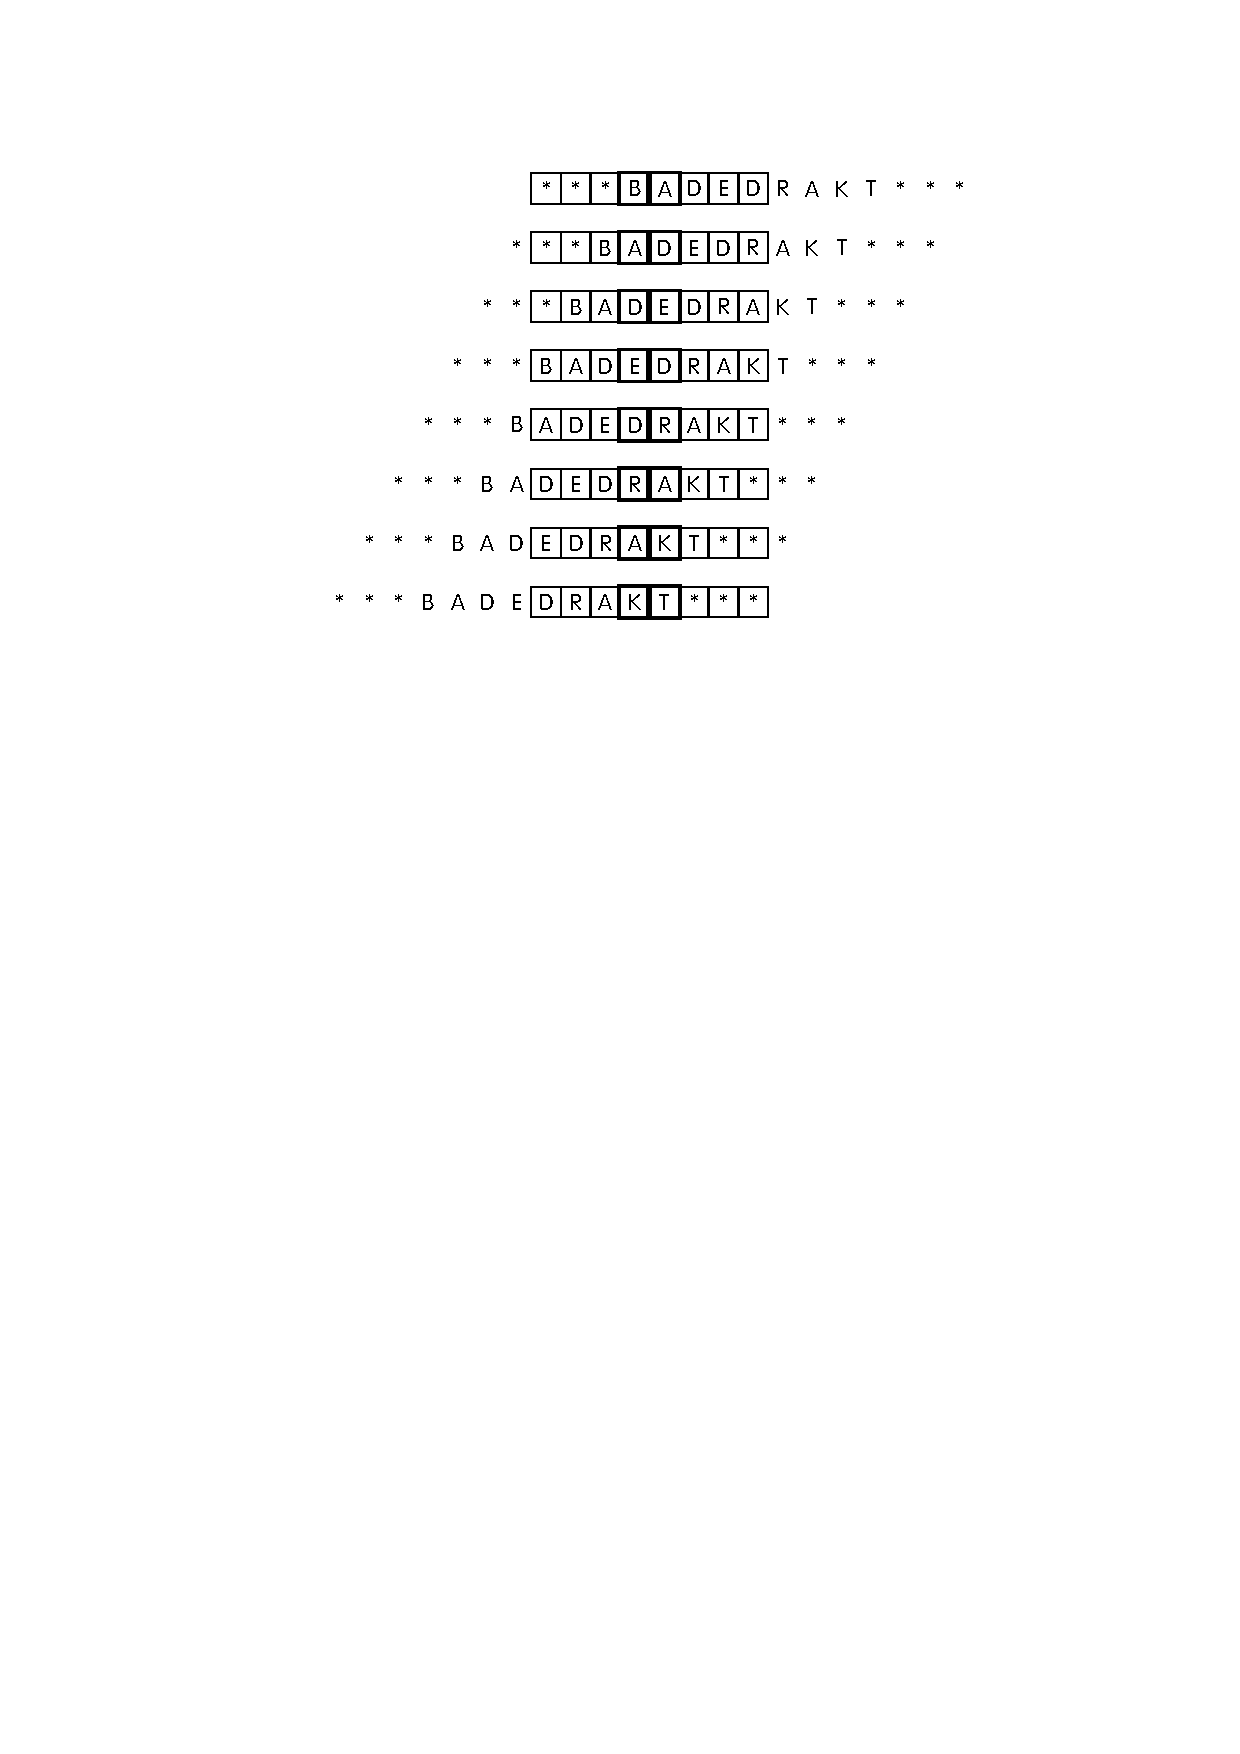
\includegraphics[width=0.75\textwidth]{content/figures/vindu.pdf}
  \caption[Vindu for orddeling med nevrale nettverk]{Vindu som viser hvordan nettverket tester et ord for hvor delepunkter skal settes inn. Illustrasjon hentet fra \textit{Two approaches to hyphenating norwegian} \cite{kristensen1998two}.}
  \label{fig:vindu}
\end{figure}


Når nettverket er tilstrekkelig opplært kan vi presentere nye ord for nettverket og det vil kunne svare om det sannynligvis er ønsket med et delepunkt. Jo større vindu og større nettverk man velger jo mer nøyaktige svar får man, men nettverket vil også vokse i lagringsstørrelse. Det vil nærme seg et oppslagsverk. Riktig vindusstørrelse og størrelse på nettverket må velges for å oppnå den beste oppveingen. 

%\subsubsection{Back-propagation}
%
%[TODO: Husk å forklare hvor dette kommer fra, kanskje hente fra AI-bok]
%
%Prosesseringselementene (nodene?) i et back-propagation-nettverk organiseres i lag, der nevronene i ett lag mottar signaler direkte fra laget under og sender signaler videre til laget direkte over. Det er ikke tillatt med koblinger innad i samme lag, bortsett fra input-laget. Inputverdien til en node $j$ regnes ut fra
%
%\begin{equation}
%S_j = \sum w_{ji}a_i
%\end{equation}
%
%hvor $w(j_i)$ er vekten mellom $j$ til $i$ og $a_i$ er output fra node $i$ i forrige lag. Utverdien fra en node er
%
%\begin{equation}
%a_j = f(S_{j})
%\end{equation}
%
%hvor $f(x)$ typisk er sigmoidalfunksjonen
%
%\begin{equation}
%S(t) = \frac{1}{1+e^{-t}}.
%\end{equation}
%
%\subsubsection{Læringsfasen}
%
%Ved første oppstart vil koblingene i nettverket få utdelt tilfeldige vekter. For å lære opp nettverket mates så inn patterns (mønstere) og vektene justeres deretter. Dette foregår ved at en definerer en input (pattern) og en ønsket output (target). Så kjører man input gjennom nettverket, ser på hva som faktisk kommer ut av resultat (output), sammenligner output med target, beregner feil og justerer vektene deretter. Det man ønsker å oppnå er et sett med vekter så nettverket tilfredsstiller alle input og output-par. Feilen i nettverket (dissonansen mellom ønsket output (target -- $t$) og faktisk output (output -- $a$)) regnes ut ved:
%
%\begin{equation}
%E = \frac{1}{N}\frac{1}{2}\sum\limits_{p}\sum\limits_{i}(t_{pi}-a_{pi})^2
%\end{equation}

\subsubsection{Orddeling via nevrale nettverk}

Kristensen og Langmyhr \cite{kristensen1998two} presenterer en metode for orddelingsproblemet ved nevrale nettverk. Problemet formuleres som et ja/nei-spørsmål om det er lovlig å putte inn et delepunkt mellom to bokstaver i et ord. Ved et ord på $n$ bokstaver får $n-1$ slike spørsmål å svare på. Nettverket får ikke se hele ordet av gangen, men et vindu av en gitt lengde med bokstaver hvor ordet ruller forbi. Tomme felter i vinduet representeres med asteriks-tegnet «*». Størrelsen på vinduet kan endres, men generelt har man at større vindu vil generere mindre konflikter og mer nøyaktige resulateter, men resultere i lengere treningstid og større minnebruk. 

Hver bokstav representeres av ett nevron (altså tjueni for norsk) og ett for asterisk-tegnet. Hvert tegn vil derfor ha en lik lengde på 30 bit. Størrelsen på output-laget vil kun være ett nevron (ja eller nei), mens input-laget vil være $V$ (størrelse på vinduet) multiplisert med $\beta$ (størrelse på alfabet). Kristensen og Langmyhr velger et vindu på 8 og antall nevroner i første lag blir da, $8\times 30 = 240$. Om vi får delepunkt i midten av vinduet, mellom de to gitte bokstavene, avgjøres om aktiviteten av output-nevronet er større en grenseverdien $0,5$. 

Treningsdataen i dette eksemplet vil bestå av ni linjer, åtte til hver bokstav i vinduet og siste til output-refereanseverdi. Eksempelvis, har vi treningsmønsteret \texttt{***|SE|KVE}, som spesifiserer at det er uønsket med delepunkt mellom \texttt{S} og \texttt{E}, representeres det på måten illustrert i figur~\ref{fig:ordmonst}. I kapittel~\ref{sec:dag-tex}, som tar for seg tidligere areid, viser resultater fra denne fremgangsmåten.

\begin{figure}
\begin{verbatim}
000000000000000000000000000001
000000000000000000000000000001
000000000000000000000000000001
000000000000000001000000000000
000001000000000000000000000000
000000000001000000000000000000
000000000000000000001000000000
000001000000000000000000000000
0
\end{verbatim}
\caption[Eksempel på treningsmønster for nevrale nettverk]{Eksempel på treningsmønster for sekvensen \texttt{***|SE|KVE}.}
\label{fig:ordmonst}
\end{figure}


\section{Regelbaserte metoder}

De regelbaserte orddelingsalgoritmene tar grunnlag i de offisielle orddelingsreglene for et gitt språk, og prøver så godt det lar seg gjøre å klassifisere ord inn i grupper og påføre de gjeldene reglene.

Los Angeles Times utviklet en regelbasert orddelingsalgoritme som skulle brukes i deres system for tekstsetting. Algoritmen registrerte og klassifiserte ord inn i vokal- og konsonantmønstere, som igjen ble delt inn i fire forskjellige grupper hvor de gjeldene reglene ble påført. I tilegg la de til regler for spesielle tilfeller og regler for håndtering av prefiks- og suffiksregler. Denne tilnærmingen ble beskrevet til å være 85--95 prosent nøyaktig. \cite{liang1983word} De nevner her ikke hvor mange feiltreff denne algoritmen generelt sett har. 

Slike tilnærminger kan ha flere svakheter. Først av alt er det en svært lite generell tilnærming til problemet. Forskjellige språk kan ha svært forskjellige regler for orddeling, og algoritmene må enten drastisk tilpasses eller skrives helt på nytt for å kunne benyttes med et annet språk. En slik tilnærming er også problematisk for språk hvor delepunktet er basert på uttale av ordet, slik som amerikansk-engelsk. Uttale kan raskt endre seg over tid, og da er man nødt til å endre selve algoritmen for å omfavne disse nye endringene. Det holder ikke å endre noen parametere, eller kjøre et program med ny inputdata for å tilpasse resultatet, slik det kan være mulig med de andre tilnærmingene. Et annet problem er at det alltids finnes unntak fra regler og en liste som utfyllende skal beskrive alle unntak kan bli unødvendig stor og vanskelig å håndtere. Til sist, sammensatte ord, som vi har mye av i det norske språket, kan være vanskelig for en datamaskin å analysere korrekt. Hvordan skal en datamaskin kunne forstå at «fylkestrafikksikkerhetsutvalgssekritariatslederfunksjonene» er en sammensatt kombinasjon av mange ord og at den må finne alle disse sammensettningene for å finne riktig delepunkt? For ikke å nevne at den også må gjennkjenne komposisjonsfuger i ordet. \cite{liang1983word,thoresen1993virtuelle}
	\section{Problemer ved automatisk orddeling}

I dette kapittelet ser vi nærmere på de delene ved orddeling og automatisk orddeling som er problematisk. Først ser vi på det som gjør orddeling vanskelig, deretter ser vi på manglene i dagens løsninger for orddeling.

\subsection{Automatisk orddeling er vanskelig} % Orddeling er prob-lemfylt

Vi mennesker opplever stort sett orddeling som et lite vanskelig eller ikke-eksisterende problem. Selv om vi kanskje ikke har full kjennskap til alle de gjeldene reglene for orddeling har vi en viss følelse for hvordan det skal gjøres. Vi har i hvertfall en forståelse for hva som er en uheldig deling av et ord. Vi har kjennskap til konteksten som ordet opptrer i og vil derfor ikke dele et ord slik at ordet kan endre betydning i seg selv og dermed betydningen av setningen. I tillegg så er vi stort sett fornøyd med å finne ett delingspunkt i et ord, det er sjeldent vi trenger flere. Det er noe som gjør at selv om vi ikke kjenner til alle reglene, så vil vi stort sett dele ordet i et punkt vi hvertfall vet er riktig. 

For datamaskiner er denne virkeligheten litt annerledes. Det er veldig vanskelig for en datamaskin å forstå konteksten hvor et ord dukker opp, noe som kan føre til uheldige og misvisende eller komiske ordbilder. Kristiansand Avis hadde en slik uheldig overskrift der ordet bokskatter ble delt i overskriten som: «i kø for boks-katter på salg» (se figur~\ref{fig:boks-katter}).

\marginelement{
\includegraphics[width=\marginparwidth]{content/figures/boks-katter.jpg}
\captionof{figure}[Eksempel på uheldig orddeling]{Problematisk orddeling i Kristiansand Avis.}
\label{fig:boks-katter}
}

Selv om datamaskinen har tilgang til informasjon om å finne delepunktet i sammensatte ord, så vil det for den være sidestilt med sammensetningen bok-skatter og boks-katter. Den har ingen kunnskap om at sistnevnte er en mindre vanlig og uheldig sammensetning og at det heller var førstnevnte deling som passet i konteksten. For et menneske er dette umiddelbart gjennkjennelig.

Eksempelet i figur~\ref{fig:boks-katter} viser hvordan ordet endrer betydning ut i fra hvordan det deles. Men vi har også tilfeller hvor ord deles som \textit{lei-ebil}, som ikke gir ny betydning til ordet, men som er en ikke spesielt pen eller heldig deling. Dette er ikke delinger som er direkte feil i henhold til de gjeldene reglene for orddeling, men det er en deling som folk vil syntes er noe merkelig. Vi ønsker i størst mulig grad delinger som gjør lesingen lett og i minst mulig grad distraherer lesere vekk fra innholdet i teksten. Dette bildet er dog ikke helt sort-hvitt og vi mennesker kan bruke ukonvensjonell orddeling til å bevisst skape morsomme og/eller iøyenfallende ordbilder, slik IKEA ganske effektivt gjorde i sin kampanje for deres juletallerken (se figur~\ref{fig:ikea}).

Homografer\sidenote{Homografer er ord som skrives likt, men med forskjellig betydning.} byr også på problemer for en datamaskin som skal prøve å dele dem. Igjen er det viktig med en forståelse av konteksten til ordet for å kunne dele det riktig. Eksempelvis har vi homonymet \textit{snekker} som skal deles forskjellig, basert på betydningen.

\ex{snek-ker}{(håndtverkeren)}\newline
\exx{snek-k-er}{(båttypen)}

\begin{figure}[h]
\centering
\includegraphics[width=0.75\textwidth]{content/figures/jul-etallerken.pdf}
\caption[Kreativ orddeling]{Kreativ orddeling i IKEAs juletallerken-kampanje.}
\label{fig:ikea}
\end{figure}

\subsection{Dagens løsninger har mangler}

Løsningene som eksisterer i dag fungerer stort sett godt, spesielt hvis man ser på amerikansk-engelsk, hvor reglene for orddeling er av annen karakter enn i norsk. Der ser en heller på utalle av ord når man velger delepunkt, og man ønsker at uttalen av ordet ikke skal endre karakter om det må deles. De første systemene som ble utviklet for å løse dette problemet er basert på amerikansk-engelsk orddeling, og mye av det vi ser i dag av komersielle produkter er varianter av disse metodene som ble utviklet den gang.

Tekstsettingssystemet \TeX{}, utviklet av Donal Knuth, var tidlig ute med å inkludere en velfungerende algoritme for automatisk orddeling. I første omgang, i \TeX{}78, ble det implementert en regelbasert algoritme. Den fant 40 \% av orddelingene med 1 \% feil. \cite{sojka1995hyphenation} Senere utviklet Liang en ny mønsterbasert løsning, patgen, som fungerte sammen med Knuths algoritme for å brekke paragrafer inn i linjer. Denne nye algoritmen har rundt 89 \% korrekte delinger, og i Liangs ord, «essentially no error[s]». \cite{liang1983word} Algoritmen for automatisk orddeling som disse to kom frem til viste seg å være så vellykket at varianter av deres løsning fortsatt brukes i stor skala i andre applikasjoner fra komersielle produkter som InDesign \cite{liang1983word} til åpen kildekode-løsninger som OpenOffice \cite{nemeth2006automatic}. Problemet, spesielt for \TeX{} sin del er at løsningen ble utviklet med det amerikansk-engelsk språket i tankene, hvor hensyn til andre språk med andre og mer kompliserte regler ble tilsidesatt.

Artikkelen \textit{New hyphenation techniques in Omega} \cite{omega} lister opp noen av \TeX{} sine feil og mangler når det kommer til andre språk, samt funksjonalitet som ville vært å foretrekke. Her kommer en rask gjengivelse.

\begin{items}
\item Ingen automatisk støtte for orddeling som fører til endring eller innskytning av ny bokstav. 

	\ex{backen → bak-ken}{(tysk)}\newline
	\exx{fotballag → fotball-lag}{(norsk)}

\item Endring av farge eller font av ordet vil føre til at orddeling ikke utføres. Dette skyldes den tekniske modellen som brukes for hvordan ord behandles av linjebrekkealgoritmen til \TeX{}.
\item \TeX{} trenger å vite på forhånd hvilke språk som skal benyttes for å kunne dele ordene riktig. Orddelingsmønsterene tilbredes og lagres i en fil som må defineres for \TeX{} og lastes inn på forhånd, som gjør det vanskelig med flere språk i én og samme tekst.
\end{items}

Videre nevner også artikkelen funksjonalitet som er ønsket av systemer som \TeX{}, i forbindelse med orddeling, som enda ikke er tilgjengelig.

\begin{items}
\item Prioriteringer av delingspunkter i et ord. I de norske reglene for orddeling har vi ikke definert prioriteringer for hvor ord bør deles, de er alle likestilte. Men det kan for eksempel være ønskelig å først prioritere å dele i hovedbindeleddet i et sammensatt ord, fremfor for eksempel prefikset. Tysk derimot har slike prioriteringer der man 
\begin{inparaenum}[\itshape a\upshape)]
\item først ønsker å dele mellom hovedbindeleddet i et sammensatt ord, dernest 
\item inne i siste komponent av et sammensatt ord, eller sist 
\item inne i en av de andre komponentene av ordet.
\end{inparaenum}
\item Vekting av orddelingspunkter. For eksempel fransk har en slik vekting av hvor ord burde deles. Man skal aldri dele etter prefikset \textit{con}, med mindre ordet ikke kan deles andre steder.
\item En form for brukerinteraksjon ved homografer som skal deles. Som i eksempelet beskrevet tidligere med \textit{snekker}, hvor det er vanskelig for datamaskinen å vite hvor ordet skal deles, kunne det vært ønskelig at bruker ble spurt om hvilken deling som er korrekt.
\end{items}
	\chapter{Tidligere arbeid}

I dette kapittelet vil vi se nærmere på tidligere arbeid, som er relevant for problemstillingen. Dessverre er det mye hemmelighetskremmeri i forbindelse med de komersielle verktøyene for tekstsetting, som Adobe InDesign, Microsoft Word og QuarkXPress, og hvordan de løser problemer som orddeling ved linjeskift. Det kunne vært interessant å kunne sett nærmere på hvordan disse verktøyene løser problemene for norsk språk, men det lar seg ikke gjøre. Av tilgjengelig materiale som ser på orddeling for norsk eller nordisk språk, finnes det ikke veldig mye. Men jeg vil presentere to publiserte metoder, først \TeX{}-algoritmen med norske orddelingsmønstere, og en algoritme for orddeling basert på nevrale nettverk.

Videre ser jeg nærmere på datastrukturen trie, som blant annet er en viktig del av av \TeX{}-algoritmen for raske oppslag av delingsmønstere, og som vil benyttes i implementasjonen beskrevet senere i oppgaven.

Til slutt ser vi på en artikkel som beskriver metoder for å dele sammensatte ord i rotord. Dette vil være relevant for implementasjon av en regelbasert orddeler.

\section{Orddeling}
\label{sec:tid-arb-orddeling}

I denne seksjonen ser vi nærmere på \TeX{}-algoritmen, mønstergenerering med patgen og de norske orddelingsmønsterene som er tilgjengelig. Til slutt ser vi på en sammenligning av resultatene fra orddeling med \TeX{} opp mot et løsning basert på nevrale nettverk (beskrevet i kapittel~\ref{sec:nevrale-nettverk}).

\subsection{Orddelingsalgoritmen i \TeX{}}

I dagens \TeX{}-system brukes et mønsterbasert system for orddeling, utviklet av Franklin Mark Liang \cite{liang1983word}. Algoritmen \cite[s.~449--450]{knuth1986texbook} støtter seg på en liste (trie, se kapittel~\ref{sec:trie}) med forskjellige mønstere, unikt tilpasset hvert språk. Et eksempel fra den norske mønsterlisten:

\ex{.fem5o6g5}{}

Punktum markerer slutt eller start på et ord, mens tallene spesifiserer om det er ønskelig med et delepunkt på gitt plassering. Oddetall betyr at det er ønskelig med delepunkt, mens partall sier det ikke er ønskelig. Ved større tall, vektes disse høyere. Hvis vi ønsker å dele ordet «hyphenate» finner vi alle mønstre som passer helt eller som er en substreng av ordet, og teller opp den totale summen av vektede punkter for så kunne bestemme hvor ordet kan deles.

\ex{\texttt{he2n}}{}\newline
\exx{\texttt{hena4}}{}\newline
\exx{\texttt{hen5at}}{}\newline
\exx{\texttt{hy3ph}}{}\newline
\exx{\texttt{1na}}{}\newline
\exx{\texttt{n2at}}{}\newline
\exx{\texttt{4te.}}{}\newline
\exx{Ord: hyphenate}{}\newline
\exx{Orddeling: hy-phen-ate}{}

Slik vil vi få vektede tall som beskriver hvor det er ønskelig med delepunkt og hvor det ikke er ønskelig (ikke lov) med delepunkt. Ordet hyphenate blir delt som hy-phen-ate, som er korrekt i følge amerikansk-engelsk orddeling.

\subsubsection{Mønstergenerering}

For at \TeX{}-algoritmen skal kunne dele ord, trenger den en mønsterliste over orddelinger for hvert språk. Frank Liang har utviklet programmet patgen som utfører denne jobben \cite{liang1983word}.

Ved oppstart trenger patgen tre filer: en translate-fil som definerer alfabetet som skal benyttes, pattern-filen som eventuelt inneholder tidligere mønstere og dictionary-filen som er orddelingslisten med alle delte ord, som vil ligge til grunne for mønstergenerereringen. 

Patgen gjør flere gjennomkjøringer av orddelingslisten. Hver gjennomkjøring kalles et nivå. Dette er de samme nivåene (oddetall -- delepunkt, og partall -- ikke delepunkt) beskrevet i avsnittet om \TeX{}. Når programmet først starter er man på nivå null, siden det enda ikke er generert noen lovlige delepunkter i mønsterlisten. Ved hver gjennomkjøring i hvert nivå må man bestemme følgende verdier:

\begin{description}
\item[hyph\_start] Minste lengde på mønster som blir behandlet på gjeldende nivå.
\item[hyph\_finish] Største lengde på mønster som blir behandlet på gjeldende nivå.
\item[good\_wt] Vekt som brukes i formel for å bestemme om et delepunkt skal danne et mønster.
\item[bad\_wt] Vekt som brukes i formel for å bestemme om et delepunkt skal danne et mønster.
\item[threshold] Grenseverdi som bestemmer om delepunkt skal danne mønster.
\end{description}

For enkelthets skyld kan vi si at vi setter hyph\_start og hyph\_finish begge til tre. Det betyr at ved dette nivået skal vi kun se på mønster ved lengde tre. Når patgen løper gjennom listen for dette nivået, vil den eksempelvis telle alle tilfellene av substrengen \textit{tio}. La oss si at dette resulterte i funn av $1793$ like mønstere, hvor det i $1793$ av tilfellene var tillatt med et delepunkt før \textit{-tio}, mens i de resterende $20$, ikke var tillatt. Disse tallene vil da gi verdiene til variablene \texttt{good} og \texttt{bad}. Når vi har talt og funnet dette for alle mulige mønstere for orddelingslisten har vi det vi trenger for å regne ut om mønsteret skal med i den endelig listen eller ikke, ved hjelp av formelen:

\begin{equation}
\label{eq:patgen}
\textit{good} \times \textit{good\_wt} - \textit{bad} \times \textit{bad\_wt} \geq \textit{threshold}
\end{equation}

Ved en uendelig bad\_wt vil man sørge for at kun trygge mønstere blir valgt, der $\text{bad} = 0$. Men de fleste tilfeller velger man en overveielse over de to som virker hensiktsmessig. Men for å forhindre mønstre i å ønske å dele ord på unøskede (bad) steder, kan vi legge til et nivå (her nivå to) som fungerer som et unntak til nivået under. Det vil ofte være vanlig å da velge mønstre av lengre lengde på nivået over. Slik kan man alternere med nivåer som unntak til unntak, i maks ni nivåer. Et typisk mønster vil være \textit{1en} på nivå én, siden det er veldig mange -en-endelser. Men dette mønsteret vil da dele ordet \textit{gren} feil som \textit{gr-en}. Vi kan da på nivå to legge inn et unntaksmønster \textit{gr2en}, som vil forhindre algoritmen fra å dele ordet på dette punktet. Om dette blir et gjeldene mønster avhenger da av minste og største mønsterlengde på nivået og vektene og grenseverdien som brukes i formel~\ref{eq:patgen}. 

Hvordan man velger verdiene som skal brukes ved hvert nivå er ikke helt lett å si, og bunner ut i mye prøving og feiling. Som Liang selv sier i sin avhandling om generering av mønstre for amerikansk-engelsk, «We do not have any theoretical justification for these parameters; they just seem to work well» \cite{liang1983word}. 

\subsubsection{Norske mønsterlister}

Det har vært flere iterasjoner med generering av norske orddelingsmønsteret til bruk i \TeX{}-systemet. De tre viktigste kan vi se oppstilt i tabell~\ref{tab:patterns}. Første, \textit{nohyph.tex}, ble fremstilt for hånd av Ivar Aavatsmark, og følger norske orddelingsregler slik de var formulert før endringene i 1973 \cite{nohyphbx, thoresen1993virtuelle}. Forsøk på å dele ord etter dagens regler med denne mønsterlisten resulterte i  74,99 \% riktige delte ord, 3,15 \% feilaktig delte ord og 25,01 \% ord som ikke ble delt \cite{thoresen1993virtuelle}. \textit{nohyph2.tex} ble fremstilt av Lars Gunnar Thoresen i forbindelse med hans masteroppgave i 1993 \cite{thoresen1993virtuelle}. Denne mønsterlisten ble laget på grunnlag av et utvalg av ord fra et tekstkorpus av skjønnlitteratur, nyhetsstoff og faglitteratur som ble kjørt gjennom programmet patgen. Med dette oppnådde Thoresen 90,5 \% korrekt deling, 0,97 \% feil deling og 9,5 \% delepunkter som ikke ble funnet. Dagens gjeldene liste er \textit{nohyhbx.tex}, fremstilt av Rune Kleveland og Ole Michael Selberg \cite{nohyphbx}, og inneholder 27149 mønstere. Det er ikke tilgjengelig målinger for nøyaktigheten til disse nye mønsterlistene, og jeg har forsøkt å komme i kontakt med dem for å oppdrive dette, men det har ikke lykkes. 

\begin{table}
\centering
\begin{tabular}{rlll}
\hline
\multicolumn{1}{l}{\textbf{Navn}} & \textbf{G} & \textbf{B} & \textbf{M} \\ \hline
\textbf{nohyph.tex}                 & 74,99 \%   & 3,15 \%    & 25,01 \%   \\ \hline
\textbf{nohyph2.tex}                & 90,5 \%    & 0,97 \%    & 9,5 \%     \\ \hline
\textbf{nohyphbx.tex}               & --         & --         & --         \\ \hline
\end{tabular}
\caption[Oversikt over orddelingsmønstere for \TeX{}]{Nøyaktigheten til de forskjellige norske orddelingsmønsterene tilgjengelig for \TeX{}-systemet. nohyphbx.tex er de nyeste norske mønstrene tilgjengelig for \TeX{}, og vi kan anta at de har noe bedre resultater en nohyphbx.tex. Mønstrene i nohyphb og nohyphbx deler, i samsvar med tradisjonen, ord med tilføyd bøyningsendelse eller suffiks slik at siste konsonant går til neste linje (hu-set), men åpner vanligvis ikke for deling mellom rot og bøyningsendelse (hus-et). \cite{nohyphbx}}
\label{tab:patterns}
\end{table}

\subsection{Sammenligning av \TeX{}-algoritmen og nevrale nettverk}
\label{sec:dag-tex}

Dag Langmyhr og Terje Kristensen \cite{kristensen1998two} har utført en sammenligning av \TeX{}-orddelingsalgoritmen og en metode for orddeling basert på nevrale nettverk, utviklet ved Høyskolen i Bergen. Deres resultater viser at \TeX{}-algoritmen er et bedre valg hvis man kan legge til grunne en stor nok ordliste for mønstergenereringen. Ved en liten ordliste (8000 ord), med ord kjent for algoritmene gjennom treningsprosessen, gjør nevrale nettverk en mye bedre jobb med 78 \% av alle lovlige delepunkter funnet (av kjente ord) og 0,0 \% ulovlige delepunkter funnet, enn hva \TeX{} gjør. \TeX{} gjør en særdeles dårlig jobb med 70 \% av lovlige delepunkter funnet, og hele 88 \% ! ulovlige delepunkter. Når størrelsen på ordlisten økes til 40 000 ord ser vi \TeX{} gjør en bedre jobb. 90 \% av alle lovlige delepunkter blir funnet (mot det nevrale nettverket sine 94 \%), og kun 0,3 \% ulovlige delepunkter blir funnet (mot det nevrale nettverket sine 6,8 \%). Det viktigste er å redusere gale delepunkter funnet.
 
\section{Trie}
\label{sec:trie}

Trie-strukturen\sidenote{Trie uttales som det engelske ordet «try», men stammer fra ordet re\textit{trie}val.} er en viktig del av implementasjonen av den mønsterbaserte \TeX{}-algoritmen for orddeling, både for hastighet og for plassbesparing. Den vil også være en viktig del av implementasjonen beskrevet senere, for rask søk i ordlister. Derfor gis det en introduksjon til denne datastrukturen. Teksten er basert på innholdet i boken \textit{Data Structures and Algorithms in Java} \cite{goodrich2014data}.

Trie er en svært effektiv datastruktur for mønstergjennkjenning. Mens andre algoritmer for mønstergjennkjenning (som KMP-algoritmen) baserer seg på en preprosessering av strengen som skal gjenkjennes i en tekst (for økt hastighet), baserer trie seg på en preprosessering av selve teksten som vi ønsker å søke etter strenger i. Det betyr at en trie-struktur vil ha en dyr oppstarstkost, men som kompenseres med svært effektive oppslag. Dette gjør at strukturen egner seg godt i tilfeller med en fast tekstmengde der man har behov for å gjøre mange og raske oppslag av strenger og uttak av informasjon.

\subsection{Oppbygning av en trie-struktur}

En trie representerer et sett $S$ med strenger $s$ fra et definert alfabet $\sum$. Den bygges opp som en trestruktur $T$ der alle noder, untatt rotnoden, er markert med en bokstav fra alfabetet $\sum$. Hver barnenode til en intern node av $T$ er markert med en unik bokstav fra $\sum$. Det er altså ikke lov med noder på samme nivå representert av en lik bokstav. Treet $T$ har $s$ antall bladnoder, hver assosiert med en streng fra $S$, slik at vi ved å kjede sammen alle bokstavene fra nodene langs stien fra rotnoden til bladnoden $v$ danner den orginale stringen fra $S$ assosiert med bladnoden $v$. Si illustrasjon \ref{fig:trie} for et eksempel. 

\begin{SCfigure}[H]
\centering
\tikzset{
  treenode/.style = {align=center, inner sep=0pt, text centered,
    font=\sffamily},
  arn_r/.style = {treenode, circle, draw=black, text=gray, 
    text width=1.5em, very thick},% arbre rouge noir, noeud rouge
  arn_x/.style = {treenode, rectangle, draw=black,
    minimum width=1.6em, minimum height=1.6em, very thick, text=gray}% arbre rouge noir, nil
}

\begin{tikzpicture}[->,>=stealth',level/.style={sibling distance = 5cm/#1,
  level distance = 1.5cm}] 
\node [arn_r] {}
    child{ node [arn_r] {$a$} 
            child{ node [arn_r] {$n$} 
		child{ node [arn_x] {$d$}}
		child{ node [arn_x] {$e$}}
            }                        
    }
    child{ node [arn_r] {$o$}
            child{ node [arn_r] {$k$} 
							child{ node [arn_r] {$s$}
								child{ node [arn_x] {$e$}}
							}
							child{ node [arn_r] {$t$}
							child{ node [arn_r] {$a$}
							child{ node [arn_x] {$n$}}
							child{ node [arn_x] {$v$}}
							}
							}
            }
            child{ node [arn_r] {$s$}
							child{ node [arn_x] {}}
							child{ node [arn_r] {$t$}
								child{ node [arn_x] {}}
								child{ node [arn_r] {e}
								child{ node [arn_x] {r}}
								}
							}
            }
		}
; 
\end{tikzpicture}
\label{fig:trie}
\caption[Eksempel på triestruktur]{Triestruktur som representerer ordene «and», «ane», «okse», «oktan», «oktav», «os», «ost» og «oster». Bladnoder er indikert ved en firkant.}
\end{SCfigure}

Et krav for en trie er at ingen strenger er substrenger av andre strenger i $S$. For å kunne tillate dette, at strukturen skal kunne representere for eksempel både «os» og «ost», kan vi legge til en bokstav som bladnode som ikke eksisterer i $\sum$. Slik vil vi kunne representere substringer, men fortsatt tilfredstillet kravet. I figuren over er dette representert med tomme bladnoder. Se for eksempel «os» og «ost», som begge er substrenger av «oster».

\subsubsection{Kompleksitet}

Ved søk etter en streng i en triestruktur traverserer vi nedover i nodene etter bokstavene som representerer vår streng $x$. Hvis traveseringen av streng $x$ ender i en bladnode (indikert ved en firkantnode i illustrasjonen over) har vi et treff. Ut i fra dette kan vi se at søketiden for en streng med lengde $m$ gir en øvre grense på $O(m\cdot |\sum|)$. Altså, for hver bokstav i streng $x$ av lengde $m$, må vi se gjennom alle barnenodene til en gitt node i stien, som i værste tilfelle kan være $|\sum|$ antall noder, på hvert nivå. Ved optimalisering av søk i barnenoder, for eksempel via en hashtabell, kan søk på hver nivå reduseres til $O(1)$, og den totale kompleksiteten blir $O(m)$. 

\section{Analyse av sammensatte ord}
\label{sec:sammensatt-analyse}

Det vanskeligste problemet når det kommer til en regelbasert tilnærming til automatisk orddeling er å finne den korrekte hovedgrensen i sammensatte ord. Dette problemet kan deles i to deler: først finne alle mulige (lovlige) tolkninger for hvordan ordet kan være sammensatt; så velge hvem av tolkningene som (høyst sannsynlig) er korrekt.

 Artikkelen «Finding the Correct Interpretation of Swedish Compunds – a Statistical Approach» \cite{sjobergh2004finding} ser på disse problemene relatert til det svenske språk (som har samme produktive ordsammensetning som norsk). Under vil jeg gjengi metoden som ble brukte og hva de fant ut av.

\subsection{Finne alle dekomponeringer av et sammensatt ord}

For å finne alle tolkninger av et sammensatt ord har forfatterene utviklet en modifisert utgave av analyseprogrammet Stava\sidenote{Stava er et program for å finne rotordene som et sammensatt ord er bygget opp av.}. Løsningen finner kun første og beste mulige løsning, så denne ble utvidet til å finne alle mulige løsninger. Modulen fungerer som følger: 

Tre ordlister ligger til grunn: én liste over \textit{inviduelle ord} (inviduell liste) som aldri oppstår i sammensetninger; én liste over \textit{avsluttende ord} (avsluttende liste), ord som enten kan avslutte et sammensatt ord eller opptre selvstendig; og til sist en liste over \textit{begynnelsesord} (begynnende liste), med modifiserte ordstammer som enten kan forme første eller midtre del av et sammensatt ord.

For å dekomponere et sammensatte ord, gjøres da følgende:

\begin{itemize}
\item Sjekk først inviduell liste: eksisterer hele ordet her, avslutt (treff), hvis ikke gå til neste trinn.
\item Sjekk etter treff i enden av ordet i avsluttende liste: får man treff, gå til neste trinn.
\item Sjekk etter treff med første del av ordet i begynnende liste: ved treff, vi er en mulig tolkning, ellers, gjør rekursivt kall da ordet kan ha flere enn to komponenter. 
\end{itemize}

Det gjøres også et forsøk på å sette inn en binde-s mellom komponenter for å se om det gir noen treff. 

Denne metode vil gi mange mulige tolkninger som resultat, om flere eksisterer. Neste problem er da å finne hvilken av disse tolkningene som (høyst sannsynlig) er den korrekte.

\subsection{Valg av riktig tolkning}
\label{sec:sjoberg}

Jonas Sjöberg og Viggo Kann beskriver seks forskjellige metoder, samt en hybridmetode, for å velge én tolkning, som mest sannsynlig er korrekt/ønsket, ut fra flere tolkninger. Alle metodene testes med en liste over flertydige sammensatte ord.

\subsubsection{Antall komponenter}

En enkel metode som fungerer overraskende godt: Velg den ordanalysen som gir færrest rotord-komponenter. Ved flere tolkninger som gir likt antall komponenter så velges tolkningen med det lengste etterleddet. Denne metoden gir korrekt tolkning i 90 \% av tilfellene. Janne Bondi Johannesen og Helge Hauglin foreslår dette som eneste metode i deres artikkel «An automatic analysis of Norwegian compounds»\cite{johannessen1996automatic}. 

\subsubsection{Semantisk kontekst}

Idéen er: ved analyse av ordet bilderamme (når vi mener bilde+ramme), er det stor sannsynlighet at ordet bilde eller ramme alene opptrer i avsnittet rundt der ordet opptrådde. Dette ble implementert ved at man først fant alle komponeneter i det sammensatte ordet. Disse ble så gått gjennom og talt hvor mange ganger de opptrådde innenfor en vindusramme av hundre ord. Disse tallene ble så igjen vektet mot avstanden fra orginalordet til der det andre ordet opptrådde. Nærmere ga høyere vekt. Denne tilnærmingen ga det dårligste resultatet med en nøyaktighet på 72 \%. Den klarte dog å finne noen tolkninger som ingen av de andre metodene fant.

\subsubsection{Komponent-frekvens}

Denne metoden ser på frekvensen til komponentordene (forledd og etterledd) i sammensetninger; hvor ofte de opptrer i en kombinasjon. Det geometriske gjennomsnittet\sidenote{Verdien man får ved å finne produktet av de n antall tallene, for så å regne ut n-roten av resultatet.} mellom komponentene i de mulige tolkningene ble så regnet ut, og den med størst verdi ble valgt. For å forbedre resultatet ble også frekvensen til komponenter i sammensatte ord fra et korpus også tatt med i beregningen, som ga en nøyaktighet på 86 \%.

\subsubsection{Syntaktisk kontekst}

Denne metoden prøver å se på konteksten der det sammensatte ordet opptrer for å se hvilken ordklasse det sammensatte ordet høyst sannynlig tilhører. I et sammensatt ord vil etterleddet bestemme ordklassen (både for svensk og norsk). Hvert av de foreslåtte sammensatte ordene ble analysert for hvilken ordklasse de tilhørte, så ble ordet erstattet med et dummy-ord med samme leksikalske sannsynlighet og setningen tagget på nytt. Taggeren analyserer så alternativene på nytt og velger den som har størst sannsynlighet for å være riktig i denne konteksten. En slik løsning hadde en nøykatighet på 86 \%.

\subsubsection{Part of Speech of Components}

Enkelte kombinasjoner av ordklasser er mer vanlig enn andre. For eksempel substantiv-substantiv er svært vanlig (25\%), mens pronomen-pronomen-kombinasjoner stort sett aldri oppstår. Denne metoden tar nytt av dette og tagger forledd og etterledd med tilhørende ordklasse. Sannsynligheten var så beregnet som produktet mellom alle de forskjellige sannsynlighetene, og den høyeste ble valgt. Denne ble rapportert til å fungere ganske godt med en nøyaktighet på 91 \%.

\subsubsection{Bokstav-n-grammer}

Enkelte bokstavkombinasjoner opptrer ingen andre steder i et sammensatt ord enn i sammensetningsgrensen. Dette kan brukes til å dele ord. Ikke alle sammensatte ord har denne karakteristikken, men da kan vi se på sannsynlighetsforholdet for at bokstavkombinasjonen opptrer i komposisjongrensen opp mot opptreden innad i komponentordene. Dette ble gjort ved at alle 4-gram bokstavkombinasjoner ble talt opp i sammensatte ord (men ikke overlappende i komposisjonsgrensen), fra et leksikon over sammensatte ord. Frekvenser ble lagt til ved å telle ordenes opptreden i et tekstkorpus. Når man så skal finne riktig tolkning tar man alle delingsforslagene fra ordsammensetningsanalysen og henter ut frekvensene til alle 4-grammer som går over delingspunktene i de forskjellge forslagene. Forslaget med den laveste frekvens blir så valgt, siden «[it] has the splits located at the positions most unlikely to not contain a split»\cite{sjobergh2004finding}. Denne metoden fant de ut var den som ga det beste resultatet, med en nøykatighet på 91 \%. 

\subsubsection{Hybridmetoder}

Jonas Sjöberg og Viggo Kann så at metodene ofte ga forskjellige feil, og at en hybrid løsning kunne gi høyere nøyaktighet. De valgte å kombinere metoden med best treffprosen, bokstav-n-grammer, med Part of Speech of Components-metoden, kombinert med to ad-hoc-regler\sidenote{Ad-hov-reglene ble lagt til for blant annet rette opp feil ved tolkninger hvor det var dobbeltskrevet konsonant, som analysen foreslo kunne være en sammenslåing av trippelskrevet konsonant (fotball+lag). Forslag med trippelskrevet konsonant ble svært ofte favorisert på feil grunnlag, og de valgte å konsekvent se bort fra dem.}. Modellen for 4-gram ble stort sett benyttet, med mindre PoS ga et alternativ som hadde en sannsynlighet for korrekthet som var fem ganger større. Denne metoden hadde nøyaktighet på 94 \% for flertydige ordsammensetninger og 97 \% for alle sammensatte ord. 
	\chapter{Ressurser}

Det er spesielt to ressurser jeg vil støtte meg til i min testing og implementasjon av en regelbasert orddeler. Først og fremst er det behov for en tilstrekkelig stor liste over korrekt delte ord. Deretter er det behov for en god ordliste, for å kunne slå opp ord, sammen med ordets morfologiske beskrivelse.

\section{Ordelingslister}
\label{sec:ordlister}

Tilgang til ordlister som viser delepunkter i ord, er viktig når man jobber med problemer rundt automatisk orddeling ved linjeskift. De fleste prosedyrer for automatisk orddeling som er i bruk i dag har behov for en tilstrekkelig stor liste med ord, inkludert de lovlige delepunktene. Enten som en direkte oppslagsliste til en ordlistebasert algoritme, eller som data til en mønsterbasert algoritme som produserer en mer generell liste over orddelingsmønstere. 

I det første tilfellet er vi avhengig av veldig store lister. De bør være mest mulig utfyllende -- det er kun ord som eksplisitt er oppgitt i listen som kan deles. Det betyr at man også må oppgi alle bøyningsformer for ett og samme ord, som vil skape veldig store lister. 

I det andre tilfellet trenger ikke ordlistene være like store. Der ønsker man kun et tilstrekkelig og representativt utvalg av delte ord, som så kan gi grunnlag for å generere mer generelle orddelingsmønstre. Lars Gunnar Thoresen viste i sin oppgave at med en liste over 16226 ord, forøvrig delt for hånd, var tilstrekkelig for å generere mønstre med patgen, til bruk i \TeX{} sin orddelingsalgoritme, og fortsatt få tilfredsstillende resultater \cite{thoresen1993virtuelle}.

Det tredje tilfellet vi trenger slike lister til er for å kunne sjekke kvaliteten til de forskjellige metodene for automatisk orddeling. En slik test vil typisk foregå ved at man velger ut en tilstrekkelig stor mengde tilfeldig valgte ord, som man har i to lister: en delt opp, en ikke delt. Listen med ikke-delte ord kjøres gjennom programmet, som så spytter ut en liste med alle ordene, forsøkt automatisk delt. Denne listen sammenlignes så med den orginale listen som viser alle korrekte delepunkter. 

For en del andre språk har man tilgang til store, offisielle ordlister som viser alle lovlige delepunkter i ordene. Dette har vi dessverre ikke i Norge. Men noe finnes, og jeg vil her kort beskrive de ordlistene som meg bekjent er tilgjengelig, og hva de kan tilby i denne konteksten. 

\begin{description}
\item [Edd]	Eining for digital dokumentasjon har tilgjengelig på sine nettsider flere ulike søkbare databaser\footnote{\url{http://www.edd.uio.no/}}, som blant annet inneholder informasjon om delepunkt i sammensatte ord og informasjon om komposisjonsfuger. Som med Bokmål- og Nynorskordboka bygger disse databasene og søkemotorene på data fra Norsk ordbank. Dessverre er ikke disse dataene tilgjengelig i et strukturert nedlastbart format. 
\item[Nynorsk og Bokmålsordboka] 	Nynorsk- og Bokmålsordboka er søkbare, digitalt tilgjengelige ordbøker på nett\footnote{\url{http://www.nob-ordbok.uio.no/}}. I likhet med Edd-søkemotoren bygger disse ordbøkene på data fra Norsk ordbank, men inneholder mindre informasjon om hvert enkelt ord samt inneholder kun et subset av ordene tilgjengelig i Norsk ordbank. Søkemotoren viser delepunktet i sammensatte ord, men er ikke tilgjengelig for nedlasting i sin helhet.
\item[Norsk ordbank] Norsk ordbank er en omfattende ordliste, og inneholder blant annet morfologisk beskrivelse av ordene. Denne databanken ligger til grunne for både EDD-søket og for Bokmål- og Nynorsordboka, som begge inneholder informasjon om delepunkt for hovedfugen i sammensatte ord. Men dessverre er ikke denne informasjonen inkludert i den nedlastbare og fritt tilgjengelige utgaven av ordbanken\footnote{\url{http://www.edd.uio.no/prosjekt/ordbanken/}}.
\item[NST Uttaleleksikon]	NST (Nordisk Språkteknologi AS) sto bak utviklingen av et språkleksikon. NST gikk konkurs i 2003, og i 2006 ble ressursene derfra kjøpt opp av et sameie av Universitetet i Oslo, Universitetet i Bergen, Noregs teknisk-naturvitskaplege universitet, Språkrådet og IBM for å videreføre dette. I 2009 fikk Nasjonalbiblioteket oppdraget av Kulturdepartementet å igjen videreføre dette arbeidet, for å bygge opp en språkbank og tilgjengeliggjøre innholdet. I dag er dette tilgjengelig under navnet Språkbanken\footnote{\url{http://www.nb.no/Tilbud/Forske/Spraakbanken/Tilgjengelege-ressursar/Leksikalske-ressursar}}. Dette leksikonet inneholder blant annet informasjon om dekomponering av sammensatte ord.
\item[Norsk landbruksordbok]	Norsk landbruksordbok er en ordbok over faglige uttrykk fra norsk landbruk, utgitt på det Norske samlaget i 1979. Av korrespondanse med Språkrådet ble jeg opplyst om at denne ordlisten beskrev alle delepunkter i ordene . Ordlisten er nå fritt tilgjengelig i wiki-form på nettet\footnote{\url{https://wiki.umb.no/NLO/index.php/Hovudside}}, men denne utgaven inneholder ikke informasjon om delepunkter. Jeg har ikke lykkes med å få svar fra kontaktperson for wiki-prosjektet om dataen over delepunkter er tilgjengelig. 
\item[IBM] 	På 1980-tallet stod IBM for produksjon av ordlister med delepunkter for både nynorsk og bokmål. Disse var tiltenkt bruk i stavekontroll og for systemer for orddeling. Aftenposten benyttet seg av disse listene, og når prosjektet ble avsluttet i årskiftet 1991/1992 var listen på hele $1200000$ ord. \cite{jan-engh} Jeg forhørte meg om denne listen, men den er ikke lenger tilgjengelig da de ble lagret på teip, og som Jan Engh skrev, «… men evig eies ei det teipte».
\item[Lars Gunnar Thoresen]		Lars Gunnar Thoresen skrev i 1993 en todelt masteroppgave med tittelen «Virtuelle fonter og norsk orddeling i \LaTeX{}». Han beskriver også vanskeligheter med tilgangen til tilstrekkelig store lister med ferdigdelte ord, og endte opp med å dele en liste med ord for hånd. Han valgte ut en mengde med ord han mente var representative gjennom en frekvensanalyse av en utvalgt tekstkorpus. Han valgte så videre ut ord med en viss gjennomsnittslengde. Disse ordene ble så delt manuelt etter de gjeldene reglene. Til slutt endte han opp med en liste på  $16226$ ord. \cite{thoresen1993virtuelle} Listen er tilgjengelig som et PDF-vedlegg i hans masteroppgave\footnote{\url{https://www.duo.uio.no/handle/10852/8875}}. Dessverre var denne listen lagret i PDF-en med et noe vanskelig tegnsett, kombinert med en vanskelig struktur som gjorde det vanskelig å parse dataen automatisk. For å få ut listen måtte PDF-en gjennom et tekstgjenkjenningsverktøy, før hver kolonne på de 100 sidene måtte kopieres ut manuelt. Til slutt måtte en god del ord korrigeres for eventuelle feil som oppsto på veien.
\end{description}

I mitt arbeid har jeg av disse valgt å støtte meg til listen til Lars Gunnar Thoresen. Det er den eneste av de som er tilgjengelig, som også lister en stor nok mengde ord, som forsøker i vise alle lovlige delepunkter.

\section{Norsk ordbank}

Norsk ordbank er en ordliste utviklet ved Universitetet i Oslo og finnes både for bokmål og nynorsk, tilgjengelig med en GPLv3-lisens\footnote{Ordbanken er tilgjengelig for nedlasting ved å signere skjemaet her \url{http://www.edd.uio.no/prosjekt/ordbanken/}}. Listen er laget ved en grunnordliste og bøyningsmønstere. Informasjonen er fordelt i to filer, \textit{fullform\_bm.txt} og \textit{paradigme\_bm.txt}, som jeg her vil gi en kort beskrivelse av.

\subsection{fullform\_bm.txt}

\texttt{fullform\_bm.txt} inneholder seks kolonner for hver oppføring, separert med tabulatortegn.

\begin{description}
\item[Første kolonne] Gir et unikt identifikasjonsnummer for oppføringen.
\item[Andre kolonne] Viser grunnformen av ordet, eksempelvis \textit{bil} for oppføringen \textit{bilene}.
\item[Tredje kolonne] Viser fullformen av ordet, eksempelvis \textit{bilene}.
\item[Fjerde kolonne] Gir ordet morfologisk beskrivelse, eksempelvis \textit{subst mask appell ent ub normert} for oppføringen \textit{bil}. 
\item[Femte kolonne] Viser paradigmekode, som linkes opp til en oppføring i \texttt{paradigme\_bm.txt}, hvor man kan finne videre informasjon om bøyningen av ordet.
\item[Sjette kolonne] Et ekstra referansenummer som trengs i kombinasjon med paradigmekoden, for å finne korrekt oppføring i \textit{paradigme\_bm.txt}. 
\end{description}

\subsection{paradigme\_bm.txt}

\textit{paradigme\_bm.txt} inneholder åtte kolonner for hver oppføring, separert med tabulatortegnet.

\begin{description}
\item[Første kolonne] Viser paradigmekode, som refereres til fra \textit{fullform\_bm.txt}.
\item[Andre kolonne] Gir ordets ordklasse og eventuell del av morfologisk beskrivelse.
\item[Tredje kolonne] Eventuell beskrivelse av paradigmet. 
\item[Fjerde kolonne] Om bøyingsparadigmet er fullstendig, eller for eksempel bare har entall eller flertall.
\item[Femte kolonne] Eksempel på ord med paradigmet.
\item[Sjette kolonne] Nummer i bøyningsparadigmet.
\item[Sjuende kolonne] Morfologisk beskrivelse.
\item[Åttende kolonne] Den faktiske bøying/bøyingsendelse som tillegges stammen av ordet ved bøying.
\end{description}

	\part{Regelbasert automatisk orddeling}
	\chapter{Implementasjon av en regelbasert orddeler}

I denne delen av oppgaven ønsker jeg å se på muligheten for en ny tilnærming til problemet om automatisk orddeling. Metodene som eksisterer i dag er stort sett mønsterbaserte (\TeX{}-algoritmen og de basert på nevrale nettverk). Disse har god presisjon med henholdsvis 90 og 96 prosent av korrekte delinger funnet, og 0,3 og 6,8 prosent feil delinger (se kapittel \ref{sec:tid-arb-orddeling}). Det er selvfølgelig ønskelig at korrekte delepunkter funnet er større, og spesielt at antall feil delepunkter ytterligere reduseres. En enda større mangel ved de eksisterende metodene for orddeling, er mangelen for å kunne skille på de forskjellige typer av orddeling vi har i norsk (se kapittel \ref{sec:orddelingsreglene}). Eksempelvis sier Finn-Erik Vinje i boka Skriveregler at sammensatte ord «… deles primært mellom de ordene de består av» og at «i sammensetninger med mer enn to ord (ledd) bør man dele der hovedgrensen går» \cite{vinje}. Dette er delinger de gjeldene metodene ikke har mulighet til å skille mellom. De vil generere, så langt de klarer, alle mulige delepunkter, men uten informasjon om hvilken regel som ga opphav til de forskjellige delepunktene. Derfor ser jeg det ønskelig å finne en ny tilnærming til orddelingsproblemet, som løser dette ved å gi kontroll over hvilke regler som benyttes for orddelingen, og ønskelig gir en høyere presisjon i funn av delepunkter.

I kapittel \ref{sec:automatisk-orddeling} presenterte jeg de tre hovedkategoriene av metoder for automatisk orddeling: \textit{ordlistebaserte}, \textit{mønsterbaserte} og \textit{regelbaserte}. Historisk har vi sett at ordlistebaserte tilnærminger har vært brukt, eksempelvis Aftenpostens liste over 1,2 millioner ferdigdelte ord, brukt i deres system for tekstsetting, på nittitallet. Denne metoden har åpenbare svakheter: nyord som introduseres til språket må kontinuerlig markers med delepunkter og legges til listen, og den vil ha problemer med den produktive ordsammensetningen vi har i norsk språk. Former for mønsterbaserte algoritmer er det vi i all hovedsak ser i bruk i dagens systemer for tekstsetting, som \TeX{}, OpenOffice og InDesign, og er alle basert på Donald Knuth og Frank Liangs algoritme \cite{smrvz1996word, knuth1986texbook, wiki-tex}. Også i mer akademisk sammenhenger er de fleste mønsterbaserte (nevrale nettverk) \cite{nemeth2006automatic, kristensen1998two}. De mønsterbaserte algoritmene forsøker å danne delemønstere som generaliserer større lister over korrekte delte ord. En mønsterliste som deler ord perfekt, vil i all praktisk forstand være identisk med en komplett ordliste over delepunkter. Så, for at en mønsterliste skal ha noe for seg er det nødt til å generalisere, og med en generalisering fører det til unntak hvor ord blir delt feil. Dagens mønsterbaserte algoritmer tilbyr heller ingen mulighet for økt kontroll over delepunktene, gjennom valg av orddelingsregler som skal benyttes. Den siste kategorien av orddelingsalgoritmer, de regelbaserte, har jeg ikke sett vært forsøkt rettet mot norsk språk med våre orddelingsregler. Slike tilnærminger har vært kritisert, blant annet av Fran Liang, for å være lite generelle — de må utvikles spesifikt rettet mot hvert skriftspråk med sine unike regler \cite{liang1983word}. Dette ser jeg heller som en styrke. Ved en analytisk fremgangsmåte har vi mulighet til å øke presisjonen rettet mot de gjeldene reglene for orddeling, og vi kan bevare informasjonen om reglene som gir opphav til de forskjellige delepunktene. Noe som kan gi bruker og applikasjoner kontroll til å selv bestemme hvilke regler som skal benyttes, for eksempel kun deling mellom hovedfugen i sammensatte ord, som kan sies å være deling av høyere kvalitet en for eksempel deling med enkonsonantregelen. Jeg vil derfor benytte meg av sistnevnte tilnærming.

\section{Arkitektur}

Ved å se på reglene for orddeling (kapittel \ref{sec:orddelingsreglene}), har jeg identifisert en hovedflyt for programmet (figur \ref{fig:app-flow}). Før man kan påføre orddelingsreglene på et ord (HyphenationRules), må man først identifisere om ordet er sammensatt. Hvis det ikke er det, så skal orddelingsreglene påføres på ordet. Om ordet er sammensatt, må det deles i komponentene det er sammensatt av. Dette foregår i to steg, løst basert på metoden til Sjöberg og Kann, beskrevet i kapittel \ref{sec:sammensatt-analyse}. Først blir ordet dekomponert ved hjelp av en ordliste i CompoundSplitter til alle lovlige dekomponeringer. Deretter, om det finnes fler enn én dekomponeringsmuligheter, blir det forsøkt valgt ut den dekomponeringen som mest sannsynlig er den korrekte eller ønskede. Informasjon om binde-s og binde-e tas med i betraktningen, via EphenthesisAnalyser, basert på funnene til Johannesen og Hauglin, beskrevet i kapittel \ref{sec:reg-bind}. Videre vil jeg gi en mer detaljert beskrivelse av hver modul (fremhevet i grønt i figur \ref{fig:app-flow}) i programflyten.

\begin{SCfigure}[h]
\centering

% Define block styles
\tikzstyle{decision} = [diamond, draw, fill=blue!10, 
    text width=4.5em, text badly centered, node distance=2.5cm, inner sep=0pt]
\tikzstyle{block} = [rectangle, draw, fill=green!10, text centered, rounded corners, minimum height=2em]
\tikzstyle{line} = [draw, -latex']
\tikzstyle{curve} = [draw, -latex', bend left=60]
\tikzstyle{word} = [node distance=3cm]
    
\begin{tikzpicture}[node distance = 2cm, auto, font=\footnotesize]
    % Place nodes
    \node [word] (ord) {Inputord};
    \node [decision, below of=ord] (sammensatt) {Er ordet sammensatt?};
    \node [block, right of=sammensatt, node distance=4cm] (regler) {HyphenationRules};
    \node [block, below of=sammensatt, node distance=2.5cm] (split) {CompoundSplitter};
    \node [block, left of=split, node distance=4cm] (dic) {Dictionary};
    \node [decision, below of=split, node distance=2.5cm] (flere) {Flere mulige delinger?};
    \node [block, below of=flere, node distance=3cm] (pick) {CompoundInterpreter};
    \node [block, left of=pick, node distance=4cm] (eph) {EphenthesisAnalyser};
    
    \path [line] (ord) -- (sammensatt);
    \path [line] (sammensatt) -- node {Nei}(regler);
	\path [line] (sammensatt) -- node [left] {Ja}(split);
	\path [line] (split) -- (flere);
    \draw[curve] (flere) to[bend right=20] node[left=.6em] {Nei} (regler);
    \path [line] (flere) -- node [left] {Ja} (pick);
    \path [line,dashed] (eph) -- (pick);
	\draw[curve] (pick) to[bend right=20] (regler);


\end{tikzpicture}
\label{fig:app-flow}
\caption[Programflyt for Hyphenator]{Viser programflyten til Hyphenator. Moduler er fremhevet i grønt.}
\end{SCfigure}

\subsection{Dictionary}
\label{sec:dictionary}

Dictionary-modulen fungerer som et grensesnitt mot en ordbank. Alle modulene vil ha behov for å kunne gjøre oppslag i en ordbok, og hente ut relevant informasjon, som både oppslag om ordet er representert i ordboken, og om ordenes morfologiske beskrivelse. For ordliste som ligger til grunn for denne modulen vil jeg benytte Norsk ordbank, utviklet og vedlikeholdt av Språkrådet og Institutt for lingvistiske og nordiske studier ved Universitetet i Oslo. Den er tilgjengelig som eksportert data i råtekstformat, og fritt tilgjengelig med en GPL-lisens\footnote{\url{http://www.edd.uio.no/prosjekt/ordbanken/}}. Dette er den mest omfattende ordbanken tilgjengelig, med over 1,2 millioner ord, og inkludert ordenes bøyning og morfologiske beskrivelse.

Med en stor ordliste er det viktig at ordspørringene utføres tilstrekkelig raskt. Spesielt CompoundSplitter vil gjøre en stor mengde spørringer etter ord med en øvre grense på $O(n!)$, hvor $n$ er lengden på strengen som forsøkes deles. En naiv løsning med et array vil være uakseptabel. Det vi ser er at listen over ord vil være statisk for hver kjøring, ingen nye ord vil legges til – vi trenger kun å gjøre raske oppslag. Trie-strukturen, beskrevet i kapittel \ref{sec:trie}, har rask søketid for oppslag, med øvre grense $O(m\cdot |\sum|)$ eller $O(m)$ med ytterligere optimalisering, dog noe på bekostning av oppstartstid når ordlisten skal lastes inn i trestrukturen. Men dette vil være en god oppveiing med tanke på den store mengden spørringer som må gjøres for hver kjøring. Jeg vil derfor implementere Dictionary som en trie-struktur.

Innlastningstiden til ordlisten har blitt noe optimalisert. Ved første oppstart vil ordbanken leses som vanlig fra fil, og satt inn i en trie-struktur. Denne objektstrukturen skrives så direkte til fil, som gjør at ved etterfølgende oppstart av programmet leses objektstrukturen direkte inn i minnet.

Hovedfunksjonene i grensesnittet til modulen er: 
\begin{items}
\item Utføre spørringer og hente ut ord fra ordlisten (om ordet ikke eksisterer returneres nil). Spørringer etter forkortelser (markert som fork i ordlisten) vil også returnere nil da forkortelser ikke skal deles. 
\item Hente paradigmebeskrivelsen til et ord (spesielt ordklasse og bøyningsendelse). 
\item Hente (om tilfelle) prefiks eller sufiks av et ord. Dette gjøres ved et oppslag i arrayer som inneholder prefikser og suffikser (beskrevet i kapittel \ref{sec:orddanning}) og en sjekk om noen av disse er er prefikser eller suffikser av det angitte ordet. Videre gjøres det også et oppslag om resten av strengen er et gyldig ord i ordbanken. 
\item Svare om en streng inneholder én eller fler stavelser (returnerer true eller false). Dette gjøres noe naivt ved en sjekk om strengen inneholder mer enn én vokalgruppe adskilt av konsonanter, noe som gjør at ord som «reelt» (to stavelser) blir feilaktig antatt til å ha én stavelse.
\end{items}

\subsection{CompoundSplitter}

For å kunne dele sammensatte ord etter ordleddsregelen (se kapittel \ref{sec:orddeling}) trenger vi å finne leddene som ordet består av. Dette gjøres, som beskrevet over, i to steg. CompoundSplitter gjør første steg steg i denne prosessen ved å finne flest mulige lovlige dekomponeringer av et ord.

Dette gjøres ved at strengen dekomponeres i alle mulige kombinasjoner av substrenger, hvor det så gjøres et oppslag i Dictionary-modulen om hver substreng er et gyldig ord. Hvis hver substreng-oppdeling resulterer i et gyldig ord, legges dekomponeringen til en liste over mulige løsninger. Hvis den møter på en «s» eller «e» i strengen testes det for om dette kan være en binde-bokstav (se kapittel \ref{sec:ord-bind1}). Det vil si at substreng før bindebokstav og substreng etter bindebokstav i seg selv må være gyldige dekomponeringer. Hvis dette er tilfelle legges oppdelingen til listen over mulige løsninger. Når alle oppdelinger er funnet og testet returneres listen. Jeg har valgt en noe naiv rekursiv implementasjon av denne algoritmen (blant annet kunne den inkludert memoisering for å unngå forsøk på dekomponering av samme substrenger), da jeg ser på tidsoptimalisering som en sekundær prioritert i denne oppgaven. Den rekursive funksjonen fungerer som følger (se også kodesnutt \ref{listing:compound-splitter}):

\begin{items}
\item Løp gjennom ordet fra venstre til høyre og slå opp substringen i ordlisten, hvis det ikke gir treff, fortsett, ellers;
\item hvis vi er på enden av stringen, da har vi en løsning som legges til en liste over mulige tolkninger og vi returnerer. Ellers;
\item gjør et rekursivt kall med resten av stringen (suffikset) som parameter til funksjonen.
\end{items}

\begin{listing}
\inputminted[firstline=30,lastline=68,gobble=4,linenos=true,breaklines=true,bgcolor=bar!10,fontsize=\footnotesize]{ruby}{project/hyphenator/lib/hyphenator/compound_splitter.rb}
\caption[Rekursiv dekomponeringsfunksjon for ord]{Rekursiv funksjon som deler sammensatte ord inn i alle mulige dekomponeringer.}
\label{listing:compound-splitter}
\end{listing}
\clearpage

Det ble også gjort et forsøk på å implementere tolkning av trippelskrevet konsonant (fotballag som delt skal stå som fotball+lag).  Det fungerer ved: når vi møter dobbeltskrevet konsonant hvor disse både kan tilhøre forleddet (fotball) \textit{og} hvor en kan tilhøre etterledd (fotbal[l]+lag), vil et en ekstra konsonant settes inn og et ekstra tolkningsalternativ genereres: \textit{fotball+lag}. Dette måtte jeg gå bort fra (kommentert ut i kodesnutt), da den genererte flere feil tolkninger en den løste problemer. Dette er samme konklusjon trukket av Sjöberg og Kann \cite{sjobergh2004finding}. Se kapittel \ref{sec:konklusjon} for mer detaljert diskusjon.

Resultatet fra CompoundSplitter returneres som et array med én eller fler dekomponerte strenger på formen “eple+tre” eller “hest+e+sal” ved tilfelle av bindebokstav.

\subsection{CoumpoundInterpreter}
\label{sec:comp-int}

CompoundInterpreter har som oppgave å velge ut dekomponeringen som mest sannsynlig er den korrekte eller den ønskede, når det finnes fler enn én mulig dekomponering. Dette er en kompleks prosess og ikke lett å få til helt korrekt Eksempelvis, hvordan skiller vi mellom hviken dekomponering av “førti+tall” og “før+titall” som er den korrekte? Sjöberg og Kann presenterer seks forskjellige metoder for dette, inkludert en hybridløsning (se kapittel \ref{sec:sammensatt-analyse}). Av tidshensyn velger jeg i første omgang å implementere teknikken som ser på \textit{antall komponenter} i ordet. Den har en enkel implementasjon og gir tilfredstillende med korrekte tolkninger, 90 \%. Johannesen og Hauglin presenterer også denne metoden i artikkelen «An automatic analysis of Norwegian compounds»\cite{johannessen1996automatic}. I tillegg vil jeg benytte informasjon om tolkning av fugebokstaver fra sistnevnte artikkel. Dette beskrives nærmere i kapittel \ref{sec:eph}.

\subsubsection{Valg av korrekt tolkning}
%Når det eksisterer mer en én mulig dekomponering av et ord vil den eller de tolkningene som har færrest og likt antall ledd bli valgt ut. Om det eksisterer flere tolkninger med likt antall ledd (som ofte er tilfelle) vil de bli videre analysert. Om dekomponeringen inneholder en fugebokstav vil EphenthesisAnalyser analysere ordet videre (se neste kapittel). Om ikke det er tilfellet vil tolkningen med det lengste etterleddet bli valgt og returnert som et svar. Eksempelvis er “hus+vinduene” foretrukket fremfor “husvin+duene”. 
%
%\begin{center}
%{\huge\color{gray!50}{\decofourleft}}
%\end{center}

Modulen vil motta en liste med to eller flere mulige dekomponeringer av et ord i en liste (fra CompoundSplitter). De vil da komme inn som et array. 

\ex{[“lese+sal+sturer”, “lese+sal+s+turer”]}{} 

Når en enkelt \textit{s} eller enkelt \textit{e} står alene betyr det alltid at det er en bindebokstav, siden de ikke er selvstendige ord på egenhånd, og det er ingen annen tolkning enn bindebokstav som er en lovlig tolkning hvor disse bokstavene står alene. Modulen vil gå gjennom hver og en tolkning og analysere dem. 

Det første som sjekkes er om dekomponeringen inneholder en bindebokstav, hvis den gjør det vil den bli sendt til modulen EphenthesisAnalyser (se sekjson~\ref{sec:eph}) for videre analyse. Hvis ikke dette er tilfellet går vi videre til en analyse. I første omgang vil jeg kun fokusere på å benytte meg av metoden presentert av Sjöberg og Kann \cite{sjobergh2004finding} som ser på \textit{antall komponenter} i ordet. Denne metoden er svært enkelt å implementere, men gir overraskende gode resultater (90 \% korrekt ved tvetydig input).

Metoden for å se på antall komponenter fungerer som følgende: 
\begin{inparaenum}[\itshape a\upshape)]
\item velg den av analysene som har færrest komponenter i analysen; og
\item ved tolkninger med likt antall komponenter, velg den med det lengste etterleddet
\end{inparaenum}\sidenote{Dette er også metoden Johannesen og Hauglin \cite{johannessen1996automatic} presenterer når man skal velge mellom flere mulige tolkninger. Dog nevner de ikke punkt \textit{b)}.}. Eksempelvis vil det sammensatte ordet \textit{lavastøvet}, bli dekomponert av CompoundSplitter, og sendt til CompoundInterpreter som:

\ex{lava+støvet}{}\newline
\exx{lavastøv+et}{}\newline
\exx{lava+s+tøvet}{}\newline
\exx{la+va+støvet}{}\newline
\exx{la+vas+tøvet}{}\newline
\exx{lav+as+tøvet}{}\newline
\exx{lava+stø+vet}{}\newline
\exx{lava+støv+et}{}\newline
\exx{lava+s+tø+vet}{}\newline
\exx{la+va+støv+et}{}\newline
\exx{lav+as+tøv+et}{}\newline
\exx{…}

Ved å velge alternativene med færrest antall komponenter (\textit{a)}) sitter vi igjen med to alternativer, \textit{lava+støvet} og \textit{lavastøv+et}, og ved å videre velge alternativet med lengst etterledd (\textit{b)}) sitter vi igjen med \textit{lava+støvet} -- som i de fleste tilfeller vil være den korrekte tolkningen.

Når denne modulen har valgt ut den tolkning som har den høyeste sannsynligheten for å være den korrekte, vil denne tolkningen bli sendt videre til modulen HyphenationRules, for å påføres reglenene for orddeling.

\subsection{EphenthesisAnalyser}
\label{sec:eph}

I mange tilfeller vil det være tvil om en bokstav er en bindebokstav og tilhører forleddet, eller ikke en bindebokstav og tilhører etterleddet. 

\ex{fylke\textit{s}+vei}{(bindebokstav)}\newline
\exx{øl+\textit{s}kum}{(til etterleddet)}

Det finnes mange former for fuger i norsk språk, totalt ni som jeg har identifisert (se kapittel \ref{sec:fuge-bokstav}). Ved å generere tolkninger som tar høyde for alle disse variantene av fugebokstaver kan en risikere å overgenerere antall tolkninger som til slutt fører til flere feiltolkninger en hva den løser. I følge Munthe (1972, i Johannesen og Hauglins artikkel «An automatic analysis of Norwegian compounds» \cite{johannessen1996automatic}) er 10,4 \% av alle ord i norske tekster sammensatte. Av disse er omtrent 75 \% av ordene satt sammen med en nullfuge; hvor leddene er satt sammen uten en bindebokstav. Eksempelvis “troll+øye” \cite{johannessen1996automatic}. Det betyr at rundt 25 \% av alle sammensatte ord i norsk inneholder en bindebokstav. For å kunne ta stilling til hvilke bindebokstaver jeg vil ta høyde for i både genereringen av tolkninger med bindebokstav (i CompoundSplitter) og i modulen for tolkning av bindebokstaver (EphenthesisAnalyser) så jeg det ønskelig å finne ut av en videre prosentvis fordeling av frekvensen til de forskjellge bindebokstavene (se neste kapittel, \ref{sec:fuge-frekvens}). 

\subsubsection{Frekvens av fugebokstaver}
\label{sec:fuge-frekvens}

Det finnes mange fugebokstaver, totalt åtte stykk (-s -e, -er, -en, -a, -er, -o og -ium → -ie-)  av de meg bekjent \cite{faarlund1997norsk,bindebokstaver}. Men det er nullfuge, binde-s og binde-e som er de desidert mest brukte og de resterende opptrer i mindre grad. Det vil alikevel være interessant å få noen mer konkrete tall på hyppigheten til de forskjellige bindebokstavene, slik at man kan ta stilling til dette når man skal programmere en komponent for morfologisk analyse av sammensatte ord, til bruk i en algoritme for orddeling.

Det er to analyser av frekvensbruken til bindebokstaver som kan være av interesse. Vi kan se på frekvensen som bindebokstaver opptrer i et utvalgt tekstkorpus. Da vil vi kunne se hvilke bindebokstaver som opptrer hyppigst i faktisk bruk. Et annet alternativ er å se på frekvensen til de forskjellige fugebokstavene i en ordliste. Jeg har valgt å ta for meg det siste. Det begrunnes med tidsbruk og kompleksitet ved å analysere morfologien til ord i et evneutelt tekstkorpus. Databasesøket i Eining for digital dokumentasjon, knyttet til Norsk ordbank, inneholder eget datafelt for informasjon om bindebokstaver, og det vil være relativt trivielt å hente ut disse feltene og telle frekvensen. 

For å beregne denne frekvensen gjorde jeg som følgende:

\begin{items}
	\item Det ble gjort et søk i Norsk ordbank, bokmål, med leddanalyse\footnote{\url{http://www.edd.uio.no/perl/search/search.cgi?appid=72&tabid=3174}}, med wildcard-tegnet ‘\%’ i feltet for fuger. Det vil gi meg et søkeresultat for alle ord i ordbanken som har informasjon om bindebokstaver. Dette gir et resultat med 29998 treff.
	\item Resultat pr. side endres til 30000 for å få alle resultatene samlet på en side (og får å få en lenke som inneholder alle søkekriteriene som parametere).
	\item Til sist lagde jeg et Ruby-skript som løper gjennom tabellen, spesifikt kolonne syv, som inneholder informasjon om bindebokstavene, og talte alle opptredene til de forskjellige bindebokstavene. Prosenten blir så regnet ut og resultatet vises frem.
\end{items}

Resultatet av denne kjøringen vises i tabell \ref{tab:fuge-frekvens}.

\sidetable[Frekvens over bindebokstaver]{%
Resultat som viser frekvens over bindebokstaver fra Norsk ordbank.
\label{tab:fuge-frekvens}}{%

\begin{tabular}{cr}
\toprule
\textbf{Bindebokstav} & \textbf{Frekvens} \\ \toprule
\textit{-s}                   & 83.249 \%                \\ \hline
\textit{-e}                   & 16.568 \%                \\ \hline
\textit{-me}                  & 0.087 \%                 \\ \hline
\textit{-es}                  & 0.037 \%                 \\ \hline
\textit{-a}                   & 0.047 \%                 \\ \hline
\textit{-t}                   & 0.007 \%                 \\ \hline
\textit{-æ}                   & 0.003 \%                 \\ \hline
\textit{-en}                  & 0.003 \%                 \\ \bottomrule
\end{tabular}
}

Vi ser umiddelbart at binde-s har desidert størst hyppighet med binde-e med en også betydelig prosent. Binde-en og binde-æ gir ett treff hver i databasen hvor binde-æ må være en feiloppføring da ordet er milæ*pæl, som ikke gir treff i ordboka (kun milepæl). Binde-es gir elleve treff hvor alle etterleddene er løs(het). Binde-me gir tjueseks treff i databasen, her er alle forleddene lamme- bortsett fra to som er domme og dramme.

Ut i fra dette kan vi se at det vil være en akseptabel forenkling å kun i første omgang analysere binde-s og binde-e ved en morfologisk analyse av ord som skal deles. I og med at den store majoriteten av de sammensatte ordene med bindebokstaver har en -s eller binde-e vil det også være rimelig å anta at disse vil ha enda større frekvens i et reelt tekstkorpus.

\begin{center}
{\huge\color{gray!50}{\decofourleft}}
\end{center}

\subsubsection{Hvordan fungerer modulen?}

Tolkning av bindebokstaver i sammensatte ord er et komplekst problem og det finnes ingen entydige regler for hvordan bindebokstavene opptrer. Men noen regler for binde-e og binde-s er gitt av Johannesen og Hauglin \cite{johannessen1996automatic} (beskrevet i kapittel \ref{sec:reg-bind}). Jeg vil støtte meg til disse reglene og implementere dem så langt det lar seg gjøre. For referanse gjengir jeg reglene her:

\begin{enum}
	\item Tolk sammensetningen som en kombinasjon av to rotord, uten fuge om mulig.
	
		\ex{løve-manke}{}\newline
		\exx{Ikke: løv-e-manke}{}
	
	\item Tolkning som binde-s er foretrukket om det er en tvetydig tolkning der s-en også kan ingå som første bokstav i et verbalt etterledd.
	
		\ex{aluminium-s-nakke}{}\newline
		\exx{Ikke: aluminium-snakke}{}
	
	\item Tolkning som binde-s er foretrukket fremfor nullfuge om forleddet i seg selv er et sammensatt ord.
	
		\ex{lesesal-s-turer}{}\newline
		\exx{Ikke: lesesal-sturer}{}
	
	\item Binde-s kan aldri følge binde-e og visa versa.
		
		\ex{hest-e-sal}{}\newline
		\exx{Ikke: hest-e-s-al}{}
	
	\item Ved to analyser som gir likt antall medlemmer og ingen bindebokstav er involvert, velg, hvis mulig, analysen som er et substantiv.
		
		\ex{hun-dyr}{(S)}\newline
		\exx{Ikke: hund-yr}{(V)}
	
	\item Ved to like analyser med tanke på bindebokstav og regelen over, og en av dem har et forledd som i seg selv er et sammensatt ord, velg den.
		
		\ex{fagplan-arbeid}{}\newline
		\exx{Ikke: fag-planarbeid}{}
	
	\item Binde-e kan kun settes sammen med en stamme som har enkelt stavelse.
		
		\ex{hest-e-ekvipasje}{}\newline
		\exx{tre-hest-ekvipasje}{}\newline
		\exx{Ikke: tre-hest-e-ekvipasje}{}
	
	\item Stammer kan komme før forleddet før -e så lenge de ikke danner sammensetning med forleddet.
		
		\ex{konge-hus-hest-e-ekvipasje}{}\newline
		\exx{Ikke: konge-hus-hest-ekvipasje}{}
	
	\item Binde-s opptrer ikke etter en konsonantsekvens med sibilanter … 
		
		\ex{busk-spilling}{}\newline
		\exx{Ikke: busk-s-pilling}{}
	
	\item … med mindre forleddet er sammensatt.
		
		\ex{enebærbusk-spilling}{}\newline
		\exx{enebærbusk-s-pilling}{}
	
	\item Hvis forleddet er ukjent, velg analysen med det lengste etterleddet.
		
		\ex{Ibsen-stykket}{}\newline
		\exx{Ikke: Ibsens-tykke}{}
	
\end{enum}

Videre vil jeg gi en kort beskrivelse for hvordan hver av reglene håndteres i EphenthesisAnalyser-modulen: 
\begin{inparaenum}[ 1)]
\item Tolkes indirekte ved at CompoundSplitter vil generere begge alternativer og CompoundInterpreter velge alternativ (a) om tolkningene har likt antall ledd og like langt eller lenger etterledd.
\item Avgjøres ved at fugebokstav tilføres etterleddet og det gjøres et oppslag i Dictionary om ordklassen er et verb. 
\item Er ikke implementert da det ble et problem med å finne ut om et ord videre er sammensatt. Det finnes svært mange korte ord i norsk, eksempelvis «le» og «se» som gjør at selv korte ord som «lese» kan tolkes som en sammensetning av «le+se» (se kapittel~\ref{sec:konklusjon} for videre diskusjon). 
\item Slik CompoundSplitter er implementert vil det aldri bli tolket to sekvente fugebokstaver. 
\item Denne regelen angår ikke binde-s og binde-e som modulen analyserer og er ikke tatt i betrakting (dog kunne den vært inkorporert i CompoundInterpreter, se kapittel~\ref{sec:konklusjon}). 
\item Regelen angår ikke bindebokstaver og er ikke tatt med i betraktningen. Den strider også i mot regelen om å velge tolkningen med lengste etterledd beskrevet i kapittel \ref{sec:comp-int} (se kapittel~\ref{sec:konklusjon} for nærmere diskusjon). 
\item Forleddet blir sjekket om det inneholder én eller fler stavelser. Hvis det er flere stavelser går bindebokstaven til etterleddet. 
\item Regelen er problematisk å tolke programatisk, da det er vanskelig å skille om ledet danner en sammensetning med forleddet før binde-e eller ikke. Regelen vil ikke bli tatt høyde for. 
\item Regelen tolkes på en noe naiv måte: den eventuelle rekken av konsonanter før binde-s blir sjekket for å inkorporere eventuell «s» eller «c». 
\item Denne regelen tolkes ikke av samme grunn som regel tre og problemet med overgenerering av sammensatte ord. 
\item Systemet håndterer kun ord oppført eller satt sammen av ord oppført i ordboken.
\end{inparaenum}

Modulen mottar et array med én enkelt tolkning (inkludert eventuell binde-s eller binde-e) på formen [“øl”, “s”, “kum”], der en «s» eller «e» som opptrer alene er kandidat til en bindebokstav. Modulen returnerer etter tolkningsprosessen et array med leddene hvor kandidaten til bindebokstav enten er ført til forleddet eller til etterleddet: [“øl”, “skum”]. 

\subsection{HyphenationRules}

Siste leddet i kjeden (og den viktigste) er modulen for å dele ord. Reglene som benyttes er de gitt i Finn-Erik Vinjes Skriveregler \cite{vinje}, beskrevet i kapittel \ref{sec:orddeling}. 

HyphenationRules-modulen forventer å motta et array av ett ord i én eller flere komponenter som: [“eple”] eller [“eple”, “kake”], avhengig av om det er sammensatt eller ikke. For hvert av  leddene i ordet vil reglene for orddeling på påført (untatt ordleddsregelen for sammensatte ord som påføres til slutt). Delepunktene blir ikke direkte satt inn i ordet, men posisjonen for delepunktet blir lagret i et array. Reglene påføres på følgende måte (og rekkefølge): 
\begin{description}
\item[Unntak] Ord med tilknyttede tall (som årstall og ordenstall) skal ikke deles. Programmet antar at input er en sammenhengende streng bestående av bokstaver fra det norske alfabetet. Av den grunn trenger vi ikke ta høyde for dette. Videre skal ikke enstavelsesord deles, dette sjekkes ved hjelp av Dictionary-modulen sin funksjon som sjekker etter én eller fler stavelser. Til sist skal ikke forkortelser (eksempelvis ADHD) deles. Dette gjøres igjen ved et oppslag i Dictionary, som inneholder informasjon om ordet er en forkortelse. Hvis noen av disse kriteriene oppfylles vil ordet returneres uten delepunkter.
\item[Avledningsprefiks] Ved oppslag i Dictionary blir det sjekket om ordet er dannet med et avledningsprefiks. Hvis så er tilfelle blir posisjonen for delepunktet lagret, og prefikset fjernet fra ordet, slik at det kan bli analysert videre.
\item[Avledningssuffiks] Først sjekkes Dictionary for et eventuelt avledningssuffiks. Videre, hvis dette er tilfellet, blir det sjekket om suffikset starter på vokal eller konsonant. Hvis det starter på konsonant deler vi forran suffikset (posisjonen lagres i et array). Ved konsonant kan ikke ordet inkludert suffiks deles etter enkonsonantregelen, og suffikset fjernes derfor fra ordet, for videre analyse. Ved vokal deler vi også foran suffiks (posisjon av delepunkt lagres). Men i dette tilfellet kan hele ordet, inkludert suffiks, også deles etter enkonsonantregelen, og ordet i sin helhet kan analyseres videre.
\item[Bøyningsendelser] Ord med bøyningsendelse deles før endelsen. Dette gjøres ved et oppslag i Dictionary som inneholder informasjon om ordenes bøyning. I tilfeller med bøyningsendelse kan vi også dele etter enkonsonantregelen, så ordet returneres i sin helhet for å analyseres videre. Når stammen ender på vokal kan vi kun dele før endelse om den også starter på en vokal.
\item[Enkonsonantregelen] Til slutt påføres enkonsonantregelen på strengen som er igjen (etter eventuelle prefikser og suffikser er fjernet). Dette gjøres mekanisk ved å sørge for at det minst er en vokal per linje (før og etter hvert delepunkt) og at det kun går én konsonant til ny linje. Det betyr at når en streng prosesseres sekvensielt må vi ha sett minst én vokal og etter et eventuelt delepunkt må vi ha én konsonant etterfulgt av en vokal. Unntaket er ved enkelte konsonantforbindelser som gjengir én og samme lyd og tilhører samme stavelse, beskrevet i kapittel~\ref{sec:enkons-untak}. Da får vi delepunktet før disse forbindelsene. Dette tilfredstilles ved at det gjøres et oppslag i et array med unntakene ved hver kandidat for et delepunkt. Bokstaven «x» skal også alltid høre til foregående stavelse, og tilfredstilles ved en ekstra sjekk. Det er også lov å dele mellom vokaler som hører til hver sin stavelse (re-elt), men dette er komplisert å løse problematisk. Se kapittel~\ref{sec:konklusjon} for ytterligere diskusjon.
\end{description}

Når alle reglene er gått gjennom returneres et array som viser posisjonen til alle delepunktene funnet i ordet, og delepunktene blir satt inn i ordleddet. Dette gjøres for alle leddene som ordet er satt sammen av. Til slutt vil de delte leddene bli satt sammen, med delepunkt (bindestrek) mellom leddene, til en sammenhengende streng. Eksempelvis vil ordet «eplekake», representert som [“eple”, “kake”] bli delt individuelt av reglene over slik at vi sitter med [“ep-le”, “ka-“ke”] for det hele blir satt sammen til strengen “ep-le-ka-ke” og returnert som endelig resultat.

Vi ønsker i denne modulen å finne \textit{alle} mulige delepunkter for et gitt ord. Det vil si at for eksempel ordet \textit{utvetydighetene} skal returneres som \textit{u-t-ve-ty-dig-he-t-e-ne}:

\ex{utve-tydighetene}{(deler mellom sammensetningene)}\newline
\exx{u-tve-tydighetene}{(deler etter prefiks)}\newline
\exx{u-tve-tydig-hetene}{(deler før suffiks)}\newline
\exx{u-tve-tydig-het-ene}{(deler før endelse)}\newline
\exx{u-t-ve-ty-dig-he-t-e-ne (enkonsonantregelen)}{}


\section{Ytelse}

Det har ikke blitt tatt nevneverdig hensyn til ytelse og eksekveringstid i denne implementasjonen. Prosjektet er ment i første omgang som et «proof of concept» for å se om en slik tilnærming til automatisk orddeling lar seg gjennomføre. Eksempelvis kunne implementasjonen vært utført i et kompilert programmeringsspråk for økt ytelse. Se kapittel \ref{sec:kildekode} for ytterligere diskusjon av valg av implementasjonsspråk. Videre er implemetasjonen av CompoundSplitter noe naiv i sin rekursive virkemåte. Ved å introdusere memoisering\sidenote{Memoisering er en optimaliseringsteknikk for å mellomlagre resultater fra kostbare funksjonskall, slik at det lagrede resultatet kan returners ved ny, identisk inndata \cite{wiki-memo}.} til funksjonen kan eksponentiell kjøretid reduseres til polynomisk kjøretid.

En optimalisering har dog blitt gjort. Ved første implementasjon av Dictionary-modulen ble ordlisten på 1,2 millioner ord lagret i et array. Dette gjorde at CompoundSplitter fikk en svært høy eksekveringstid (spesielt på grunn av manglende memoisering), på opptil 25 minutter minutter for en listen på omtrent 150 ord. Ved å gå over til en trie-struktur gikk eksekveringstiden for CompoundSplitter ned til 0,26 sekunder for en tilsvarende liste. Dog økte innlastingstiden for ordlisten fra rundt 15 sekunder til omtrent ett minutt. Dette er tålelig da listen kun lastes inn én gang ved oppstart av programmet. Ved å lagre trie-objektet direkte til fil, for så å lese objektet direkte inn i minnet, ble innlastingstiden ytterligere redusert til rundt 45 sekunder.


\section{Kildekode}
\label{sec:kildekode}

Selve Hyphenator-applikasjonen består av 888 linjer kode fordelt på fem filer (se mappen \texttt{lib/hyphenator/} i figur \ref{fig:source-code}). Moduler og alle tester er programmert i programmeringsspråket Ruby\sidenote{Ruby er et dynamisk, objektorientert og generelt programmeringsspråk \cite{wiki-ruby}.}. Valget ble gjort på grunnlag av de mange bibliotekene som er tilgjengelig, spesielt for håndtering og manipulering av strenger, for å få en mest mulig effektiv implementasjonsfase. Dynamiske språk, som Ruby, har noen negative egenskaper, spesielt knyttet til eksekveringstid, da koden tolkes og utføres i kjøringen. Egenskapen om enkel og effektiv implementsajon ble valgt fremfor lavere eksekveringstid da dette prosjektet, som nevnt over, er et «proof of concept».

\begin{figure}
\begin{verbatim}
|-hyphenator/
  |-data/
  |  |-ordbank_bm
  |  |  |-dataformat.txt
  |  |  |-fullform_bm-utf8.txt
  |  |  |-fullform_bm.txt
  |  |  |-fullform_bm_trie.txt
  |  |  |-gpl.txt
  |  |  |-opphavsrett.txt
  |  |  |-paradigme_bm-utf8.txt
  |  |  |-paradigme_bm.txt
  |  |-tests
  |  |  |-complex-interpreted-compounds.txt
  |  |  |-complex-splitted-compounds.txt
  |  |  |-hyphenated-non-compounds.txt
  |  |  |-hyphenated-words.txt
  |  |  |-simple-interpreted-compounds.txt
  |  |  |-simple-splitted-compounds.txt
  |-lib
  |  |-hyphenator
  |  |  |-compound_interpretor.rb
  |  |  |-compound_splitter.rb
  |  |  |-dictionary.rb
  |  |  |-ephenthesis_analyser.rb
  |  |  |-hyphenation_rules.rb
  |  |-hyphenator.rb
  |  |-utils
  |  |  |-string.rb
  |-tests
  |  |-1.txt
  |  |-2.txt
  |  |-3.txt
  |  |-4.txt
  |  |-5.txt
  |  |-6.txt
  |  |-test_all.rb
  |  |-test_compound_interpreter.rb
  |  |-test_compound_splitter.rb
  |  |-test_hyphenation_rules.rb
\end{verbatim}
\caption[Filstrukturen i Hyphenator-prosjektet]{Figuren viser en oversikt over mappestrukturen og filene i prosjektet. Mappen \texttt{data/} inneholder datasettet fra Norsk Ordbank samt testordlister, i \texttt{lib/} finner vi implementasjon av modulene, og til sist, i mappen \texttt{tests/} ligger resultater og programkode for å teste implementasjonen.}
\label{fig:source-code}
\end{figure}
	\chapter{Empirisk studie av regelbasert orddeler}

I dette kapittelet ser vi på testingen av Hyphenator-programmet. Først spør vi hvilke spørsmål vi ønsker svar på, og definerer problemstillingene for oppgaven. Deretter blir metodene og målene for testene diskutert. Til slutt i dette kapittelet presenteres resultatene, før vi avslutter med en diskusjon rundt funnene og knytter dem opp til problemstillingene. 

\section{Problemstilling}

Det er mange aspekter som kunne vært testet, men det er spesielt to spørsmål som er interessante å få svar på i denne sammenhengen.

\begin{quote}
PS1: Hvor godt utfører modulene oppgavene sine hver for seg?
\end{quote}

Det vil være interessant å se nærmere på modulene i isolasjon med egne testkriterier og tester. Med dette vil det være mulig å identifisere svakheter i enkeltmoduler i programflyten, og kan fungere som en pekepinn på mulig videre arbeid for å forbedre programmet.

\begin{quote}
PS2: Hvor god kvalitet og kontroll får vi på orddelingen?
\end{quote}

Her ønsker vi å få svar på hvor vellykket løsningen er for å dele ord, samt eventuell hvilken økt kontroll vi kan få over orddelingsvalgene.

\section{Metode}

I forbindelse med \term{PS1} er det følgende moduler som er av interesse å teste: CompoundSplitter: \textit{hvor godt finner den alle mulige dekomponeringer av et sammensatt ord?} CoumpoundInterpreter: \textit{i hvor stor grad velger den riktig tolkning ved flere muligheter?} Og HyphenationRules: \textit{hvor godt påfører den reglene på ikke-sammensatte ord?} Dictionary og EphenthesisAnalyser vil ikke bli testet, da førstnevnte kun vil fungere som en hjelpemodul, og sistnevnte testes indirekte gjennom CompoundInterpreter. Ved \term{PS2} vil helheten av programmet og samspillet mellom modulene testes.

\subsection{PS1}

Her ser vi på metodikken benyttet for å belyse spørsmålet som er formulert i \term{PS1}, hvor vi ønsker å se nærmere på modulene individuelt.

\subsubsection{CompoundSplitter}

Denne modulen har som oppgave å dekomponere sammensatte ord til alle lovlige dekomponeringer, hvor ønsket dekomponering er en del av resultatmengden. Modulen vil utsettes for to tester. En \term{triviell test}, som består av 152 enkelt sammensatte ord. Det vil si ordsammensetninger som typisk har nullfuge og består av to rotord. Dette for å teste hvor godt modulen fungerer i de enkleste tilfellene, som også er formen til majoriteten (75 \%) av alle sammensatte ord i norsk \cite{johannessen1996automatic}. Den andre testen vil være en \term{kompleks test}, bestående av 27 sammensettninger som kan ha flere rotordkomponenter, samt kan inneholde binde-s eller binde-e. Slik får vi testet mer komplekse, sammensatte ord, som kan være mer vanskelig å dekomponere korrekt. De fleste av sammensetningene er hentet fra Hauglin og Johannesen \cite{johannessen1996automatic}, som er konstruerte eksempel for å illustrere spesielt vanskelige ordsammensetninger med og uten bindebokstav.

Vi registrerer et resultat som korrekt når ønsket dekomponering er en del av resultatmengden som returneres fra modulen.

\ex{eplekake}{(inndata, ønsker eple+kake)}\newline
\exx{[[ep, le, kake], [eple, kake]] (gyldig løsn.)}{}

\paragraph{Mål} I denne komponenten ønsker jeg å finne \textit{alle} lovlige dekomponeringer, og at ønsket dekomponering er en del av løsningsmengden. Denne testen bør resultere i opp mot 100 \% korrekte resultater. 
	
\subsubsection{CoumpoundInterpreter}

For denne modulen ønsker jeg å gjøre to tester: én med enkle sammensatte ord med nullfuge fra Norsk ordbank, da denne formen for komposisjon er det desidert mest frekvente (75 \% av alle sammensatte ord har nullfuge\cite{johannessen1996automatic}). I test nummer to kommer jeg til å bruke en liste over ekstra problematiske sammensatte ord som er to- eller flertydige, og som eventuelt inneholder binde-s eller binde-e. Flere av disse eksemplene vil jeg hente fra Johannesen og Hauglin \cite{johannessen1996automatic}, da flere av disse er konstruert for å illustrere vanskelighetene ved sammensatte ord med bindebokstaver. Slik vil også modulen EphenthesisAnalyser bli testet indirekte.

Hva som er en korrekt tolkning av et sammensatt ord er ikke helt enkelt å gi et entydig svar på. Men et kriterium er at det bør være mest mulig likt slik et menneske intuitivt ville tolket det. \textit{Lesesals+turer} fremfor \textit{lesesal+sturer} og \textit{dop+lager} fremfor \textit{do+plager} (tolkning som er litt mer i gråsonen). Mange av disse tolkningene vil være kontekstavhengig, som kan gjøre det vanskeligere for leseren å tolke.

\paragraph{Mål} Siden jeg støtter meg på metodene til Sjöberg og Kann \cite{sjobergh2004finding} bør det forventes å kunne få like god tall som hans enkleste, men også effektive, metode som kun ser på \textit{antall komponenter i tolkningen} (prøver å redusere). Resultatene hans ga 90 \% korrekte tolkninger ved analyse av sammensatte ord med flere mulige tolkninger (flertydige). Vi introduserer også en noe mer avansert tolkning av bindebokstaver enn det Sjöberg og Kann gjør, så det bør forventes bedre resultat enn 90 \% i begge tester.

\subsubsection{HyphenationRules}

For å isolere ut denne modulen og teste nøyaktigheten til den alene, vil jeg konstruere en liste med ikke-sammensatte ord, som jeg også deler manuelt etter reglene for orddeling. Ordlisten for ikke-delte ord vil bli matet inn i modulen, og forsøkt delt. Så gjøres det en sammenligning mellom resultat og den hånddelte listen av ord. Der vil jeg se på prosentandelen av G (good), antall riktige delepunkter funnet, B (bad), antall falske negativer og M (missed), antall falske positiver.

\paragraph{Mål} Denne testen gjøres kun med ikke-sammensatte ord, og vil derfor være enklere å utføre siden mye av kompleksiteten ved å påføre orddelingsreglene er nettopp ved analysen av sammensatte ord. Thoresen \cite{thoresen1993virtuelle} sine resultater er en naturlig sammenligning, og det bør forventes noe bedre resultater en hva han presenterer, 90,5 \% korrekte og 0,97 \% falske positiver.

\subsection{PS2}

Helheten vil bli testet med en større liste over (sammensatte og ikke-sammensatte) ord. For å kunne sjekke om disse deles korrekt, er vi avhengig av å ha en kontrolliste over korrekte delinger vi kan sammenligne med. Som beskrevet i kapittel~\ref{sec:ordlister} er det vanskelig å få tak i lister over norske ord med alle korrekte delepunkter. Jeg vil derfor støtte meg til listen konstruert av Lars Gunnar Thoresen \cite{thoresen1993virtuelle}. Listen\footnote{Listen over delte ord er tilgjengelig som vedlegg i Lars Gunnar Thoresen sin masteroppgave på \url{https://www.duo.uio.no/handle/10852/8875}.} er konstruert av $16226$ ord valgt ut fra et representativt tekstkorpus fra skjønnlitteratur og blandet faglitteratur, allmennfaglig nyhetsstoff og faglitteratur informatikk. De mest hyppige ordene ble valgt ut gjennom en frekvensanalyse. Ved å bruke samme testdata som Thoresen, vil det også være mulig å sammenligne mine resultater med det han fikk gjennom patgen og \TeX{}-algoritmen. Som med HyphenationRules, vil jeg her se på å prosentandelen av G (good), antall riktige delepunkter funnet, B (bad), antall falske negativer og M (missed), falske positiver.

\paragraph{Mål} Igjen er det naturlig å sammenligne med resultatene til Thoresen. For at tilnærmingen jeg presenterer skal være av interesse for bruk, bør den løse oppgaven med å dele ord minst like godt. 

\section{Resultater}

Jeg ønsket først å teste alle modulene hver for seg, før jeg så testet hele systemet samlet. Dette for i større grad kunne identifisere hvor eventuelle feil oppsto og i hvilke komponenter, for så å kunne klassifisere feilene bedre. Fremgangsmåten og ønskede resultater ble beskrevet i forrige kapittel. I denne teksten vil jeg beskrive hvordan testene faktisk ble gjennomført, for så å vise resultatene og tolke resultatene.

\subsection{PS1}

Her vil jeg videre presentere resultatene knyttet til PS1 i forbindelse med modulene.

\begin{table}[h]
	\centering 
	\begin{tabular}{llrrrr} \hline 
		\textbf{Navn} & \textbf{Type} & \textbf{Korrekt} & \textbf{Feil} & \textbf{(Av)} & \textbf{\%} \\
		\hline \multirow{2}{*}{\textbf{CompoundSplitter}} & Enkel & 150 & 2 & 152 & 98,68 \\
		\cline{2-6} & Kompleks & 27 & 0 & 27 & 100 \\
		\hline \multirow{2}{*}{\textbf{CompoundInterpreter}} & Enkel & 89 & 6 & 95 & 93,68 \\
		\cline{2-6} & Kompleks & 70 & 12 & 82 & 85,36 \\
		\hline 
	\end{tabular}
	\caption[Oppstilling av testresultater av moduler]{Oppstilling av resultatene fra testing av CompoundSPlitter og CompoundInterpreter, knyttet til PS1.} \label{tab:module-test} 
\end{table}

\subsubsection{CompoundSplitter}

Av tabell~\ref{tab:module-test} ser vi at modulen fikk alle riktige for den komplekse testen, og 98,68 \% riktig på den enklere testen. De to feilene som oppsto i den enkle testen er følgende (diskutert i kapittel \ref{sec:disk-ps1}):

\ex{acappella+sang}{(feil: acapellasang)}\newline
\exx{av+hør}{(feil: av+hør)}

\subsubsection{CompoundInterpreter}

Testen av CompoundInterpreter med enkelt og kompleks test, ga korrekt resultat i  henholdsvis 93,68 \% og 85,36 \% av tilfellene. Resultatet diskuteres videre i kapittel~\ref{sec:disk-ps1}, hvor også eksempler av feiltolkninger listes opp.

\subsubsection{HyphenationRules}

HyphenationRules-modulen ble testet med én liste med ikke-sammensatte ord. Resultatet vises i tabell~\ref{tab:hyphenation-results}. Prosentvis gir det G, B, M på henholdsvis 98,03 \%, 0,98 \% og 1,96 \%. Tre feil oppsto. «ar-be-id» ble delt som «Ar-beid», grunnet manglende implementasjon av støtte for deling mellom vokaler som hører til hver sin stavelse. «Ang-re» blir delt «an-g-re», som skyldes at det blir feiltolket «an» som et avledningsprefiks. «Vis-s-te» som blir det «viss-te». Her er jeg noe mer usikker på hvorfor «vis-s-te» deles slik det gjør i fasiten. Det kan være en feiloppføring, eller at «ste» regnes som bøyningsendelsen til ordet «vite».

\subsection{PS2}

I forbindelse med PS2 ble tre aspekter testes. Først en enkel test med ikke-sammensatte ord som tester modulen for påføring av orddelingsreglene direkte – uten å gå gjennom modulene for dekomponering. Deretter ble hele programmet testet med orddelingslisten på 16.226 ord, fra Thoresen \cite{thoresen1993virtuelle}. Resultatene kan sees i tabell~\ref{tab:hyphenation-results}. I forbindelse med den komplette testen, ble også eksekveringstid registrert. Det ga 45 sekunder for innlasting av ordliste i trie-struktur, og 36 sekunder for deling og resultatsammenligning av alle $16226$ ord. 

\begin{table}[h]
	\centering 
	\begin{tabular}{llrrrr} \hline 
		\textbf{Navn} & \textbf{Type} & \textbf{G} & \textbf{B} & \textbf{M} & \textbf{(Av)} \\
		\hline \textbf{HyphenationRules} & Enkel & 100 & 1 & 2 & 102 \\
		\hline \textbf{Hyphenator} & Komplett & 31439 & 3694 & 7507 & 38946 \\
		\hline 
	\end{tabular}
	\caption[Resultater fra test av Hyphenator-programmet]{Oppstilling av resultatene fra enkel og komplett test av orddelingsalgoritmen. Enkel test er utført med kun ikke-sammensatte ord, komplett test består av 16.226 ord hentet fra Thoresen \cite{thoresen1993virtuelle}. G (Good) beskriver antall korrekte delepunkter funnet, B (Bad) beskriver falske negativer og M (Missed) beskriver falske positiver.} \label{tab:hyphenation-results} 
\end{table}

Siste aspekt som skulle testes var i forbindelse med kontroll over delepunkter og orddelingsregler benyttet. Her skulle egentlig alle orddelingsreglene testes individuelt. Av tidshensyn har kun ordleddsregelen om deling i sammensetningsfugen av sammensatte ord blitt testet. Dog kan det poengteres at dette er en av de viktigste reglene, som gir de peneste delingene med minst rom for forvirrende ordbilder (slik de andre reglene, spesielt enkonsonantregelen kan skape). Resultatet fra testen er stilt opp i tabell~\ref{tab:ordleddsregelen}.

\begin{table}[h]
	\centering 
	\begin{tabular}{lrrrr} \hline 
		\textbf{Navn} & \textbf{G} & \textbf{B} & \textbf{M} & \textbf{(Av)} \\
		\hline \textbf{Ordleddsregelen} & 24 & 9 & 6 & 30 \\
		\hline 
	\end{tabular}
	\caption[Resultater fra test av ordleddsregelen]{Oppstilling av resultatet fra test av ordleddsregelen. Tegnforklaringen er den samme som beskrevet i tabell~\ref{tab:hyphenation-results}} \label{tab:ordleddsregelen} 
\end{table}

\section{Diskusjon}

I resten av kapittelet vil vi vende tilbake til de to problemstillingene, og diskutere dem knyttet opp til resultatene presentert tidligere. Til slutt tar vi et kritisk blikk på eget arbeid.

\subsection{PS1: Hvor godt utfører modulene oppgavene sine hver for seg?}
\label{sec:disk-ps1}

Av tabell \ref{tab:module-test} kan vi se at modulen CompoundSplitter fungerer svært godt. Den komplekse testen får korrekt resultat for alle sammensatte ord, mens den enkle testen får 98,68 \% korrekte resultater, med kun to feil. Disse feilene er mulig å rette opp. Første feil er ordet «avhør», som ikke returnerer som «av+hør». Dette skyldes at «av» blant annet er listet i ordboken som en forkortelse (for audio-visuelt), og dermed vil Dictionary-modulen si at oppslaget av ordet ikke er et gyldig ord. Dette kan enkelt løses ved at modulen svarer at det er et gyldig ord, så lenge det finnes minst én oppføring som ikke er en forkortelse. Den andre feilen er «acappellasang», som kun returnerer det samme ordet og ikke «acappella+sang». Dette skjer fordi ordlisten ikke har «acappella» som en oppføring for seg selv. I slike tilfeller hvor eventuelt deler av et sammensatt ord ikke er kjent for ordboken, foreslår Johannesen og Hauglin at man søker etter det lengste prefikset eller suffikset av strengen som er kjent for ordboken, og deler ordet i denne fugen. Eksempelvis ordet «ibsenstykket», hvor «stykket» er lengste suffiks, vil deles som «ibsen+stykket». Med begge testene oppnådde vi målet om tilnærmet 100 \% korrekte resultater.

Modulen CompoundInterpreter fungerer ikke tilstrekkelig godt nok. For den enkle testen ønsket vi å oppnå minst 97 \% korrekte tolkninger, og 94 \% for den komplekse testen. Med resultater på henholdsvis 93,68 \% og 85,36 \% ser vi at avstanden er for stor. Når Johannesen og Hauglin i tillegg hevder å få feil tolkning av sammensatte ord i kun 1,1 \% av tilfellene, ser vi her at det gjenstår en del videre arbeid for at denne modulen oppfyller kravet om å være tilstrekkelig god. Ved å studere feilresultatene fra begge testene, er det tydelig to kategorier av feil som opptrer desidert hyppigst og fører til dårlige resultater. Den første er ikke-sammensatte ord som blir tolket som sammensatte.

\ex{etter → et+ter}{}\newline
\exx{også → og+så}\newline
\exx{sier → si+er}{} 

Dette skyldes vanskeligheten med å avgjøre om et ord er sammensatt eller ikke. Dette diskuteres ytterligere i kapittelet for videre arbeid, \ref{sec:videre-arbeid}. Den andre kategorien for feil, er tolkninger hvor vi får en for høy prioritering på  valg tolkninger med det lengste etterleddet (beskrevet i kapittel \ref{sec:comp-int}). 

\ex{brakkvann → brak+kvann}{}\newline
\exx{førtitall → før+titall}{}\newline
\exx{flislegger → fli+slegger}{}\newline
\exx{hustak → hu+stak}{}\newline
\exx{blomsterholder → blomst+erholder}{}

\subsection{PS2: Hvor god kvalitet og kontroll får vi for orddelingen?}

\marginelement{
\begin{tikzpicture}
  \centering
  \begin{axis}[
        ybar, axis on top,
        %title={Sammenligning av resultater},
        ymajorgrids, tick align=inside,
        major grid style={draw=white},
        enlarge y limits={value=.1,upper},
        width = \marginparwidth,
		height = 7cm,
        ymin=0, ymax=100,
        axis x line*=bottom,
        bar width = 0.08\textwidth,
        axis y line*=right,
        y axis line style={opacity=0},
        tickwidth=0pt,
        enlarge x limits=true,
        yticklabel={\pgfmathparse{(int(\tick))}\pgfmathresult \%},
        legend style={
            at={(0.5,-0.01)},
            anchor=north,
            legend columns=-1,
            /tikz/every even column/.append style={column sep=0.5cm}
        },
        %ylabel={Prosent (\%)},
        symbolic x coords={
           Good,
           Bad,
          Missed},
       xtick=data,
       nodes near coords={
        \pgfmathprintnumber[precision=2]{\pgfplotspointmeta}
       }
    ]
    \addplot [draw=none, fill=red] coordinates {
      (Good,98.03)
      (Bad,0.98)
      (Missed,1.96) };\label{meg}

    %\legend{Meg,Gunnar}
  \end{axis}
  \end{tikzpicture}
    \captionof{figure}{Oppstilling av resultater fra den enkle testen av orddelingsalgoritmen gjort på en liste over ikke-sammensatte ord.}
    \label{fig:simple-result}
}

Målet for kvalitet, det vil si antall positiver (G), antall falske negativer (B) og antall falske positiver (M), var satt til å være minst like gode som Lars Gunnar Thoresen sine resultater for sine norske orddelingsmønstere for \TeX{}-algoritmen. Resultatene fra den enkle teste, bestående av ikke-sammensatte ord, ga gode resultater (se figur~\ref{fig:simple-result}). Prosentvis mengde falske negativer (B) er så og si identisk med Thorsen sine resultater (0,97~\%). Samtidig finner vi en stor andel flere positiver (G). 

I figur~\ref{fig:results} kan vi se en sammenstilling av resultatene fra den komplette testen av samme ordliste, bestående av $16226$ ord, som Thoresen benyttet seg av. Her ser vi konsekvent at resultatene for Hyphenator slår dårligere ut enn sammenligningen. Spesielt er antall falske negativer uakseptabelt høy. For en orddelingsalgoritme er det viktigere med lavest mulig antall feil delepunkter, enn det er å finne alle mulige delepunkter. Når ord skal deles ved linjeskift, trenger vi stort sett bare ett korrekt delepunkt. Mens et feil delepunkt kan fort føre til et misvisende eller komisk ordbilde.

\begin{figure}[h]
	\begin{tikzpicture}
  \centering
  \begin{axis}[
        ybar, axis on top,
        %title={Sammenligning av resultater},
        ymajorgrids, tick align=inside,
        major grid style={draw=white},
        enlarge y limits={value=.1,upper},
        width = \textwidth,
        height = 6cm,
        ymin=0, ymax=100,
        axis x line*=bottom,
        bar width = 0.08\textwidth,
        axis y line*=right,
        y axis line style={opacity=0},
        tickwidth=0pt,
        enlarge x limits=true,
        yticklabel={\pgfmathparse{(int(\tick))}\pgfmathresult \%},
        legend style={
            at={(0.5,-0.01)},
            anchor=north,
            legend columns=-1,
            /tikz/every even column/.append style={column sep=0.5cm}
        },
        %ylabel={Prosent (\%)},
        symbolic x coords={
           Good,
           Bad,
          Missed},
       xtick=data,
       nodes near coords={
        \pgfmathprintnumber[precision=2]{\pgfplotspointmeta}
       }
    ]
    \addplot [draw=none, fill=red] coordinates {
      (Good,80.72459302624146)
      (Bad,9.48492784881631)
      (Missed,19.27540697375854) };\label{meg}
   \addplot [draw=none,fill=bar] coordinates {
      (Good,90.50) 
      (Bad,0.97)
      (Missed,9.50) };\label{gunnar}

    %\legend{Meg,Gunnar}
  \end{axis}
  \end{tikzpicture}
  \caption[Sammenstilling av resultater fra \TeX{} og Hyphenator]{Sammenstilling av resultater fra Hyphenator (\ref{meg}) og \TeX{}-algoritmen (\ref{gunnar}) med mønstere fra Lars Gunnar Thoresen. Good, antall positiver funnet, ønsker vi høyest mulig, mens Bad, antall falske negativer og Missed, antall falske positiver, ønsker vi lavest mulig.}
  \label{fig:results}
\end{figure}

Når det gjelder aspektet om kontroll og hvilke regler som benyttes over delepunkter og type delepunkter ønsket, var intensjonen å sette opp individuelle tester for alle reglene. Slik kunne vi fått et bedre bilde over grad av kontroll over delepunktene som ønskes. Av tidshensyn har vi gått bort fra dette, og kun utført en test av ordleddsregelen. Dog kan det argumenteres for at dette er den viktigste av reglene, som gir de «vakreste» delepunktene. Hvis deling etter ordleddsregelen utføres riktig vil muligheter for misvisende eller komiske ordbilder, slik vi kan se i figur~\ref{fig:dopalger} og \ref{fig:freskukens}, reduseres. Resultatet fra tetsten av ordleddsregelen er fremstilt i figur~\ref{fig:ordleddsregelen}. Resultatene, spesielt antall falske negativer (Bad) er ikke tilfredstillende. Men testen er svært liten og det er derfor vanskelig å konkludere entydige. Større og fler tester av reglene individuelt trengs.

\marginelement[-6]{

\includegraphics[width=\marginparwidth]{content/figures/forord-doplager.jpg}
\captionof{figure}[Eksempel på uheldig orddeling i Dagbladet]{Faksimile, Dagbladet Nett 25. september 2013. Eksempel på uheldig orddeling som fører til et komisk ordbilde. Trolig en feil ved ordleddsregelen og en feiltolkning at ordet er satt sammen av «do» og «plager». Kilde: \url{http://www.dagbladet.no/2013/09/25/nyheter/utdanning/narkotika/innenriks/29445603/}}
\label{fig:dopalger}
}

\marginelement[14]{
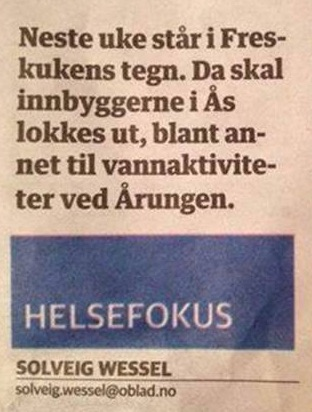
\includegraphics[width=\marginparwidth]{content/figures/freskukens.jpg}
\captionof{figure}[Eksempel på uheldig orddeling i Østlandet Blad]{Faksimile Østlandets Blad. Nok et eksempel på en uheldig orddeling. Muligens siden «fresk» eller «freskukens» var et ukjent ord for orddelingsprogrammet, og ordet ble delt etter enkonsonantregelen. Dette er en lovlig, men svært uheldig orddeling.}
\label{fig:freskukens}
}

\begin{figure}[h]
\centering
\begin{tikzpicture}
  \centering
  \begin{axis}[
        ybar, axis on top,
        %title={Sammenligning av resultater},
        ymajorgrids, tick align=inside,
        major grid style={draw=white},
        enlarge y limits={value=.1,upper},
        width = \marginparwidth,
		height = 7cm,
        ymin=0, ymax=100,
        axis x line*=bottom,
        bar width = 0.08\textwidth,
        axis y line*=right,
        y axis line style={opacity=0},
        tickwidth=0pt,
        enlarge x limits=true,
        yticklabel={\pgfmathparse{(int(\tick))}\pgfmathresult \%},
        legend style={
            at={(0.5,-0.01)},
            anchor=north,
            legend columns=-1,
            /tikz/every even column/.append style={column sep=0.5cm}
        },
        %ylabel={Prosent (\%)},
        symbolic x coords={
           Good,
           Bad,
          Missed},
       xtick=data,
       nodes near coords={
        \pgfmathprintnumber[precision=2]{\pgfplotspointmeta}
       }
    ]
    \addplot [draw=none, fill=red] coordinates {
      (Good,80.03)
      (Bad,30.0)
      (Missed,19.97) };\label{meg}

    %\legend{Meg,Gunnar}
  \end{axis}
  \end{tikzpicture}
    \caption[Resultater fra test av ordleddsregelen]{Oppstilling av resultater fra test av ordleddsregelen.}
    \label{fig:ordleddsregelen}
\end{figure}

\section{Svakheter}

Enkelte svakheter ved metodene benyttet under testingen er verdt å påpeke. Det første er at testene benyttet for å teste modulene individuelt er svært små. Det skyldes tidshensyn og det faktum at disse testene er i hovedsak ment for å vise eventuelle feil med modulene under utviklingsfasen. 

Den andre svakheten er ved den store orddelingsordlisten hentet fra Thoresen. Etter en gjennomgang av de tusen første ordene oppdaget jeg enkelte ord som var delt feil, som jeg fikk rettet opp. Men det kan antas at det vil finnes tilsvarende feildelte ord i resten av listen. Et annet problem avdekket ved listen er ordene som skal ha trippelskrevet konsonant ved orddeling, ikke er oppført riktig i listen. Alle ordene er konsekvent oppført som soppo-se, tallin-je, ka-jakklubb og fjelland, når du skulle vært sopp-po-se, tall-lin-je, ka-jakk-klubb og fjell-land. Disse er nok oppført slik bevisst, siden det er et kjent problem at orddelingsalgoritmen i \TeX{} ikke støtter slik ekspandering til trippelskrevne konsonanter. Dette problemet og andre problemer med \TeX{}-algoritmen, spesielt for språk som har ikke-standard orddeling, er påpekt i flere artikler \cite{sojka1995hyphenation,sojka1995notes,nemeth2006automatic,omega}.

Den tredje svakheten ligger i hvilken mønsterliste for \TeX{}-algoritmen som er valgt til sammenligning. Det er utviklet en nyere mønsterliste for norsk orddeling som nå distribueres med \TeX{}-systemet. En vil anta at disse mønstrene gir enda bedre resultater en mønstrene til Thoresen som sammenligningen gjøres mot. Men etter flere forsøk på henvedelser til forfatterene bak denne mønsterlisten lykkes det ikke å få tak i testresultatene for G, B og M-verdiene. Det ble derfor naturlig å sammenligne med Thoresen sine resultater som er tilgjengelig.


	\part{Oppsummering}
	\chapter{Konklusjon}
\label{sec:konklusjon}

Det første å legge merke til er hvor komplekst, og interessant, det tilsynelatende enkle problemet om automatisk orddeling faktisk er. For et menneske oppfattes det intuitivt, og det er enkelt å dele et ord. Når en skal forsøke å fortelle en datamaskin hvordan den kan gjøre det på egenhånd, blir kompleksiteten en helt annen. I denne oppgaven ønsket vi å utvikle en regelbasert tilnærming for automatisk orddeling for å
\begin{inparaenum}[\itshape a\upshape)]
\item øke presisjonen på delepunkter som blir funnet, ved flere korrekte delepunkter og færre gale delepunkter, og 
\item bevare informasjon om hvilke orddelingsregler som ga opphav til delepunkene, for å gi systemene for tekstsetting økt kontroll.
\end{inparaenum}
Vedrørende punkt a.) har vi ikke lykkes. Vi finner færre korrekte delepunkter og en uakseptabel mengde gale delepunkter. Når det gjelder punkt b.), har dette vist seg å være fullt mulig. Vi kan spesifisere nøyaktig hvilke av orddelingsreglene som skal benyttes for å dele et ord.

Resultatet fra arbeidet med denne oppgaven kan oppsummeres i følgende punkter:
\begin{enum}
\item Vi har gitt et overblikk over problemstillingen rundt automatisk orddeling og hvilke metoder som eksisterer, med et hovedfokus på metoder tilgjengelig for norsk. 
\item Vi har presentert detaljer for hvordan en kan implementere en modulær, regelbasert algoritme for orddeling. 
\item Vi har bidratt med kunnskap om frekvensen av forekomster av de forskjellige fugebokstavene i sammensatte ord.
\end{enum}

Basert på arbeidet med denne oppgaven vil jeg presentere de viktigste erfaringene å ta med seg videre. Til slutt, for at en regelbasert tilnærming til automatisk orddeling skal bli nyttig, trengs det en rekke forbedringer. I siste kapittel diskuterer jeg mulighetene for videre arbeid.

\section{Hva har vi lært?}

Først og fremst: automatisk orddeling er komplisert! Dette var et mer omfattende problem enn det jeg forestilte meg da jeg gikk i gang med arbeidet. Underveis har jeg møtt på mange utfordringer som kunne vært egnet som egne studier i seg selv. Blant annet: dekomponering av sammensatte ord til \textit{alle} rotordbestanddelene, tolkning av sammensatte ord, tolkning av bindebokstaver, håndtering av trippelskrevet konsonant, telling og markering av stavelser i ord, markering av affikser i ord og effektiv innlesing, og søk i store ordlister. Denne oppgaven bør sees på som en skisse for en mulig vei videre for å utvikle en fullverdig løsning og for videre testing.

For det andre: Reglene for hvordan ord skal deles er noen ganger vanskelig å tolke. Slik jeg tolker enkonsonantregelen\sidenote{Enkonsonantregelen: I ord med en eller flere konsonanter mellom vokaler går det én konsonant til ny linje \cite{vinje}.} vil o\textbf{-}ran-gu-tang være en lovlig deling. Altså at vi får én vokal alene på første linje. Men Vinje deler ordet som oran-gu-tang i sin bok. Derimot viser han eksempelet a-le-ne som korrekt, hvor dette er tilfelle. Listen over delte ord fra Lars Gunnar Thoresen \cite{thoresen1993virtuelle}, som benyttes til testing av modulene, er heller ikke konsekvent med dette. Derfor ville det vært svært ønskelig med en offisiell liste som viser korrekte delinger for å kunne utføre mer nøyaktige tester.

Til sist: det er fullt mulig å utvikle et godt fungerende program for orddeling som gir økt kontroll over hvilke orddelingsregler som skal benyttes. Men for at dette programmet skal bli nyttig i bruk, trengs det ytterligere arbeid for å øke presisjonen.


\section{Videre arbeid}
\label{sec:videre-arbeid}

For at den regelbaserte algoritmen for automatisk orddeling skal bli nyttig, trengs det mer arbeid. Systemet har en svært modulær arkitektur og er tilgjengelig med en fri lisens, som gjør det enkelt å studere og forbedre deler av systemet individuelt. Det er flere interessante spørsmål som trenger svar, og deler som trenger videre arbeid. Dette er de viktigste:

\begin{items}
\item Av resultatene ser vi at CompoundInterpreter er modulen som gir flest feil. Før å øke presisjonen til programmet vil det ha størst effekt å forbedre denne modulen. Johannesen og Hauglin \cite{johannessen1996automatic} hevder at deres program basert på de samme reglene ga feil analyse i kun 1,1 \% av tilfellene. Det tyder på at det her er stort forbedringspotensiale for modulen. I kapittel \ref{sec:fuge-bokstav} presenteres også en del karakteristikker for binde-s og binde-e, som kan være interessant å se på muligheten for å implementere i modulen.
\item For CompoundInterpreter kan det også være interessant å se på muligheten for å tolke sammensatte ord hvor deler av ordet ikke er kjent for ordboken. Johannesen og Hauglin \cite[s. 10]{johannessen1996automatic} beskriver en teknikk for dette.
\item Slik programmet er nå klarer den ikke å skille mellom sammensatte ord og ikke-sammensatte ord når de blir gitt til modulen CompoundSplitter. Norsk ordbank inneholder både sammensatte og ikke-sammensatte ord, slik at det ikke bare er å gjøre et oppslag der for å teste dette. Det fører til at selv korte ikke-sammensatte ord vil bli dekomponert til rotordene, som for eksempel «sele», «se» og «le». Bokmålsordboka på nett \sidenote{\url{http://www.nob-ordbok.uio.no/perl/ordbok.cgi?OPP=bindestrek&bokmaal=+&ordbok=begge}} har nylig innført markering av hovedfuge i sammensatte ord, eksempelvis «binde|strek». Hvis disse endringene etterhvert reflekteres i den tilgjengelige utgaven av Norsk ordbank, som ligger til grunne for Bokmålsordboka på nett, vil det da være mulig å skille mellom sammensatte og ikke-sammensatte ord ved et oppslag i ordboka.
\item Regelen om at enstavelsesord ikke skal deles krever en funksjon som kan telle antall stavelser i et ord. I det minste svare om ordet har én eller flere stavelser. I dagens løsning gjøres det noe naivt (se seksjon \ref{sec:dictionary}). Den vil eksempelvis feilaktig anta at ordet «reell» kun har én stavelse, når den har to. 
\item Knyttet til punktet over, har vi mangelen i programmet for å «dele mellom vokaler når de hører til hver sin stavelse», som er tillatt av enkonsonantregelen. 
\item I implementasjonen var vi nødt til å gå bort fra forsøk på å tolke dobbeltskrevet konsonant som ved deling blir trippelskrevet. For eksempel madrasselger, som delt blir til madrass-selger. Ved forsøk på å tolke slike tilfeller av ordsammensetninger endte vi med totalt flere feiltolkninger av sammensatte ord enn om vi unnlot dette. Det kunne vært interessant å sett på omfanget av slike tilfeller av sammensatte ord, og hvordan man eventuelt kan tolke dem korrekt.
\item Til sist, CompoundInterpreter vil forsøke å finne hovedfugen i et ord, altså «verdenscup-seiere» og ikke «[verdens+cup]+seiere». Det er tillatt å dele ord mellom alle fugene i sammensatte ord som består av tre eller fler rotord, selv om det er \textit{ønskelig} å dele i hovedfugen. Det ville vært interessant å se om dette lar seg gjøre. Men dette er et vanskelig problem å løse, man ender fort opp med en overdekomponering, eksempelvis «fagplanarbeid» som blir til «fag+plan+ar+be+id».
\end{items}




    \bibliographystyle{plain}
    \bibliography{bibliography/bibliography}
    
    \appendix
	\chapter{Hyphenator}
	
	Filene til prosjektet Hyphenator, inkludert tester og orddelingslister, er fritt tilgjengelig med en GPLv3-lisens på Github. 
	
	\url{https://github.com/eivindml/Hyphenator}
	
%	\addcontentsline{toc}{part}{\appendixtocname} \appendixpage*
%	\begin{appendices}
%
%	\end{appendices}

\end{document}
